% !TeX encoding = UTF-8
% !TeX program = xelatex
% !TeX spellcheck = en_US

\documentclass[degree=master, degree-type=professional]{thuthesis}
  % 学位 degree:
  %   doctor | master | bachelor | postdoc
  % 学位类型 degree-type:
  %   academic(默认)| professional
  % 语言 language
  %   chinese(默认)| english
  % 字体库 fontset
  %   windows | mac | fandol | ubuntu
  % 建议终版使用 Windows 平台的字体编译


% 论文基本配置,加载宏包等全局配置
% !TeX root = ./thuthesis-example.tex

% 论文基本信息配置

\thusetup{
  %******************************
  % 注意:
  %   1. 配置里面不要出现空行
  %   2. 不需要的配置信息可以删除
  %   3. 建议先阅读文档中所有关于选项的说明
  %******************************
  %
  % 输出格式
  %   选择打印版(print)或用于提交的电子版(electronic),前者会插入空白页以便直接双面打印
  %
  output = print,
  % 格式类型
  %   默认为论文(thesis),也可以设置为开题报告(proposal)
  % thesis-type = proposal,
  %
  % 标题
  %   可使用“\\”命令手动控制换行
  %
  title  = {基于强化学习的异质网络场景下\\传输策略优化},
  title* = {Transmission Strategy Optimization in Heterogeneous Network Scenarios Based on Reinforcement Learning},
  % :TODO
  % 学科门类
  %   1. 学术型
  %      - 中文
  %        需注明所属的学科门类,例如:
  %        哲学、经济学、法学、教育学、文学、历史学、理学、工学、农学、医学、
  %        军事学、管理学、艺术学
  %      - 英文
  %        博士:Doctor of Philosophy
  %        硕士:
  %          哲学、文学、历史学、法学、教育学、艺术学门类,公共管理学科
  %          填写“Master of Arts“,其它填写“Master of Science”
  %   2. 专业型
  %      直接填写专业学位的名称,例如:
  %      教育博士、工程硕士等
  %      Doctor of Education, Master of Engineering
  %   3. 本科生不需要填写
  %
  degree-category  = {计算机技术硕士},
  degree-category* = {Master of Computer Technology},
  %
  % 培养单位
  %   填写所属院系的全名
  %
  department = {深圳国际研究生院},
  %
  % 学科
  %   1. 研究生学术型学位,获得一级学科授权的学科填写一级学科名称,其他填写二级学科名称
  %   2. 本科生填写专业名称,第二学位论文需标注“(第二学位)”
  %
  professional-field  = {计算机技术},
  professional-field* = {Computer Technology},
  %
  % 专业领域
  %   1. 设置专业领域的专业学位类别,填写相应专业领域名称
  %   2. 2019 级及之前工程硕士学位论文,在 `engineering-field` 填写相应工程领域名称
  %   3. 其他专业学位类别的学位论文无需此信息
  %
  % professional-field  = {计算机技术},
  % professional-field* = {Computer Technology},
  %
  % 姓名
  %
  author  = {朱轩宇},
  author* = {Zhu Xuanyu},
  %
  % 学号
  % 仅当书写开题报告时需要(同时设置 `thesis-type = proposal')
  %
  % student-id = {2022214238},
  %
  % 指导教师
  %   中文姓名和职称之间以英文逗号“,”分开,下同
  %
  supervisor  = {王智, 副教授},
  supervisor* = {Associate Professor Wang Zhi},
  %
  % 副指导教师
  %
  % associate-supervisor  = {陈文光, 教授},
  % associate-supervisor* = {Professor Chen Wenguang},
  %
  % 联合指导教师
  %
  % co-supervisor  = {某某某, 教授},
  % co-supervisor* = {Professor Mou Moumou},
  %
  % 日期
  %   使用 ISO 格式;默认为当前时间
  %
  % date = {2019-07-07},
  %
  % 是否在中文封面后的空白页生成书脊(默认 false)
  %
  include-spine = true,
  %
  % 密级和年限
  %   秘密, 机密, 绝密
  %
  % secret-level = {秘密},
  % secret-year  = {10},
  %
  % 博士后专有部分
  %
  % clc                = {分类号},
  % udc                = {UDC},
  % id                 = {编号},
  % discipline-level-1 = {计算机科学与技术},  % 流动站(一级学科)名称
  % discipline-level-2 = {系统结构},          % 专业(二级学科)名称
  % start-date         = {2011-07-01},        % 研究工作起始时间
}

% 载入所需的宏包

% 定理类环境宏包
\usepackage{amsthm}
% 也可以使用 ntheorem
% \usepackage[amsmath,thmmarks,hyperref]{ntheorem}

\thusetup{
  %
  % 数学字体
  % math-style = GB,  % GB | ISO | TeX
  math-font  = xits,  % stix | xits | libertinus
}

% 可以使用 nomencl 生成符号和缩略语说明
% \usepackage{nomencl}
% \makenomenclature

% 表格加脚注
\usepackage{threeparttable}



% 表格中支持跨行
\usepackage{multirow}

% 固定宽度的表格。
% \usepackage{tabularx}

% 跨页表格
\usepackage{longtable}

% 算法
\usepackage{algorithm}
\usepackage{algorithmic}

% 量和单位
\usepackage{siunitx}

% 参考文献使用 BibTeX + natbib 宏包
% 顺序编码制
\usepackage[sort]{natbib}
\bibliographystyle{thuthesis-numeric}

% 著者-出版年制
% \usepackage{natbib}
% \bibliographystyle{thuthesis-author-year}

% 生命科学学院要求使用 Cell 参考文献格式(2023 年以前使用 author-date 格式)
% \usepackage{natbib}
% \bibliographystyle{cell}

% 本科生参考文献的著录格式
% \usepackage[sort]{natbib}
% \bibliographystyle{thuthesis-bachelor}

% 参考文献使用 BibLaTeX 宏包
% \usepackage[style=thuthesis-numeric]{biblatex}
% \usepackage[style=thuthesis-author-year]{biblatex}
% \usepackage[style=gb7714-2015]{biblatex}
% \usepackage[style=apa]{biblatex}
% \usepackage[style=mla-new]{biblatex}
% 声明 BibLaTeX 的数据库
% \addbibresource{ref/refs.bib}

% 定义所有的图片文件在 figures 子目录下
\graphicspath{{figures/}}

% 数学命令
\makeatletter
\newcommand\dif{%  % 微分符号
  \mathop{}\!%
  \ifthu@math@style@TeX
    d%
  \else
    \mathrm{d}%
  \fi
}
\makeatother

% hyperref 宏包在最后调用
\usepackage{hyperref}


\usepackage{graphicx}    % 用于插入图形
\usepackage{subcaption}  % 用于子图布局
\usepackage{caption}     % 用于定制标题

\begin{document}

% 封面
\maketitle

% 学位论文指导小组、公开评阅人和答辩委员会名单
% 本科生不需要
% !TeX root = ../thuthesis-example.tex

\begin{committee}[name={学位论文公开评阅人和答辩委员会名单}]

  \newcolumntype{C}[1]{@{}>{\centering\arraybackslash}p{#1}}


  \section*{公开评阅人名单}

  \begin{center}
    \begin{tabular}{C{3cm}C{3cm}C{9cm}@{}}
      刘XX & 教授   & 清华大学                    \\
      陈XX & 副教授 & XXXX大学                    \\
      杨XX & 研究员 & 中国XXXX科学院XXXXXXX研究所 \\
    \end{tabular}
  \end{center}


  \section*{答辩委员会名单}

  \begin{center}
    \begin{tabular}{C{2.75cm}C{2.98cm}C{4.63cm}C{4.63cm}@{}}
      主席 & 袁春                  & 教授                    & 清华大学       \\
      委员 & 吴志勇                  & 教授                    & 清华大学       \\
          % & \multirow{2}{*}{杨XX} & \multirow{2}{*}{研究员} & 中国XXXX科学院 \\
          % &                       &                         & XXXXXXX研究所  \\
          & 王智                  & 副教授                    & 清华大学       \\
          & 郑海涛                  & 副教授                  & 清华大学       \\
          & 肖喜                  & 副教授                  & 清华大学       \\
      秘书 & 吴XX                  & 助理研究员              & 清华大学       \\
    \end{tabular}
  \end{center}

\end{committee}



% 也可以导入 Word 版转的 PDF 文件
% \begin{committee}[file=figures/committee.pdf]
% \end{committee}

% 使用授权的说明
% 本科生开题报告不需要
\copyrightpage
% \copyrightpage[file=scan-copyright.pdf]

\frontmatter
% !TeX root = ../thuthesis-example.tex

% 中英文摘要和关键字

\begin{abstract}
随着多媒体网络应用的快速发展,网络传输速率控制策略在提升用户体验方面起着至关重要的作用。然而,现有的传输速率控制策略面临着两大挑战:一方面,网络应用场景的多样性和用户需求的异质性导致了不同应用在网络传输中的需求差异;另一方面,现有的控制策略库由于设计准则的差异,在单一策略工作时无法灵活应对不同场景和网络环境的适配性要求。因此,本研究旨在利用强化学习的决策框架,在异质网络场景下展开传输策略的优化。本文的研究内容包括两个主要方面:

(1)在云游戏场景下,设计对差异化的时延敏感度可感知的传输速率控制算法。算法提出了“时延敏感度”概念,并通过展开大规模客观数据测量确定不同的场景下内容对于敏感度的影响,确定了三类不同敏感度分类,并在每类敏感度下展开用户MOS实验确定了敏感度的量化数值,将其使用最小二乘法转换为强化学习的奖励空间部份构成。随后使用强化学习中演员-评论家方法优化不同场景下的传输速率,以实现延迟和视觉质量之间的最优平衡解,提升用户体验质量(Quality of Experience,QoE)。

(2)对于已具备策略库的多种网络任务类型,提出一种新规划范式设计。研究通过对现有通用网络控制方案展开流程重构,利用预训练语言模型(Pretrained Language Model,PLM)的决策和感知能力,结合Decision Transformer强化学习框架,实现策略的动态切换和适配网络的最佳选择,提升传输速率控制的适应性和效率。最后,该范式设计的被部署在自适应码率任务仿真系统上作为案例进行分析和评估。

本研究提出的算法和控制范式能够有效提高了云游戏等实时通信应用中的用户体验质量,并为未来在更多复杂网络环境中的应用提供了理论支持和实践方案。


  % 关键词用“英文逗号”分隔,输出时会自动处理为正确的分隔符
  \thusetup{
    keywords = {网络传输速率控制;云游戏;强化学习;预训练大模型;用户体验质量},
  }
\end{abstract}

\begin{abstract*}
  With the rapid development of multimedia network applications, network transmission rate control strategies play a crucial role in enhancing user experience. However, existing transmission rate control strategies face two major challenges: on the one hand, the diversity of network application scenarios and the heterogeneity of user demands lead to varying requirements for network transmission across different applications; on the other hand, due to differences in design principles, existing control strategy libraries struggle to flexibly adapt to different scenarios and network environments when operating under a single strategy. Therefore, this study aims to optimize transmission strategies in heterogeneous network scenarios using the decision-making framework of reinforcement learning. The research focuses on two main aspects:

(1) In the cloud gaming scenario, a transmission rate control algorithm capable of perceiving differentiated latency sensitivity is designed. The algorithm introduces the concept of "latency sensitivity" and determines the impact of different scenarios on sensitivity through large-scale objective data measurements. Three different sensitivity classifications are established, and for each sensitivity category, user MOS (Mean Opinion Score) experiments are conducted to quantify the sensitivity values. These values are then converted into the reward space of reinforcement learning using the least squares method. Subsequently, the actor-critic method in reinforcement learning is employed to optimize transmission rates across different scenarios, achieving an optimal balance between latency and visual quality, thereby enhancing the Quality of Experience (QoE).

(2) For various network task types that already possess a strategy library, a novel planning paradigm is proposed. This study reconstructs the workflow of existing general network control schemes and leverages the decision-making and perception capabilities of Pretrained Language Models (PLM), combined with the Decision Transformer reinforcement learning framework, to achieve dynamic strategy switching and optimal adaptation to the network environment, thereby improving the adaptability and efficiency of transmission rate control. Finally, this paradigm design is deployed in an adaptive bitrate task simulation system as a case study for analysis and evaluation.

The proposed algorithm and control paradigm in this study effectively enhance the QoE in real-time communication applications such as cloud gaming and provide theoretical support and practical solutions for future applications in more complex network environments.

  % Use comma as separator when inputting
  \thusetup{
    keywords* = {Network Transmission Rate Control, Cloud Gaming, Reinforcement Learning, Large Language Model, Quality User Experience},
  }
\end{abstract*}


% 目录
\tableofcontents

% 插图和附表清单
% 本科生的插图索引和表格索引需要移至正文之后、参考文献前
% \listoffiguresandtables  % 插图和附表清单(仅限研究生)
\listoffigures           % 插图清单
\listoftables            % 附表清单

% 符号对照表
% !TeX root = ../thuthesis-example.tex

\begin{denotation}[3cm]
\item[ABR] 自适应码率流媒体 (Adaptive Bitrate Streaming)
\item[Actor-Critic] 演员-评论家算法网络 (Actor-Critic Network) 
\item[BBA] 基于缓冲区的自适应码率算法 (Buffer-Based Algorithm)
\item[CC] 拥塞控制 (Congestion Control)
\item[CDF] 累积分布函数 (Cumulative Distribution Function)
\item[CNN] 卷积神经网络 (Convolutional Neural Network)
\item[DDPG] 深度确定性策略梯度 (Deep Deterministic Policy Gradient)
\item[GC] 梯度压缩 (Gradient Compression)
\item[LLM] 大语言模型 (Large Language Model)
\item[LSE] 最小二乘估计 (Least Square Estimation)
\item[LSTM] 长短时记忆模型 (Long Short-Term Memory)
\item[LoRA] 低秩矩阵分解 (Low-Rank Adaptation)
\item[MOS] 平均意见得分 (Mean Opinion Score) 
\item[MPC] 模型预测控制方法 (Model Predictive Control)
\item[MTP] 操作到画面 (Motion-to-Photon)
\item[PSNR] 峰值信噪比 (Peak Signal-to-Noise Ratio)
\item[QoE] 用户体验质量 (Quality of Experience)
\item[QoS] 客观服务质量指标 (Quality of Service) 
\item[RL] 强化学习 (Reinforcement Learning)
\item[RTC] 实时通信 (Real-Time Communication) 
\item[RTG] 预期回报 (Return-To-Go)
\item[RTT] 网络往返时延 (Round-Trip Time)
\item[SFT] 模型微调 (Supervised Fine-Tuning)
\item[SI] 空间感知信息 (Spatial Information) 
\item[TD3] 双延迟深度确定性策略梯度 (Twin Delayed Deep Deterministic Policy Gradient) 
\item[TI] 时间感知信息 (Temporal Information) 
\item[VMAF] 视频多方法评估融合 (Video Multimethod Assessment Fusion) 


\end{denotation}



% 也可以使用 nomencl 宏包,需要在导言区
% \usepackage{nomencl}
% \makenomenclature

% 在这里输出符号说明
% \printnomenclature[3cm]

% 在正文中的任意为都可以标题
% \nomenclature{PI}{聚酰亚胺}
% \nomenclature{MPI}{聚酰亚胺模型化合物,N-苯基邻苯酰亚胺}
% \nomenclature{PBI}{聚苯并咪唑}
% \nomenclature{MPBI}{聚苯并咪唑模型化合物,N-苯基苯并咪唑}
% \nomenclature{PY}{聚吡咙}
% \nomenclature{PMDA-BDA}{均苯四酸二酐与联苯四胺合成的聚吡咙薄膜}
% \nomenclature{MPY}{聚吡咙模型化合物}
% \nomenclature{As-PPT}{聚苯基不对称三嗪}
% \nomenclature{MAsPPT}{聚苯基不对称三嗪单模型化合物,3,5,6-三苯基-1,2,4-三嗪}
% \nomenclature{DMAsPPT}{聚苯基不对称三嗪双模型化合物(水解实验模型化合物)}
% \nomenclature{S-PPT}{聚苯基对称三嗪}
% \nomenclature{MSPPT}{聚苯基对称三嗪模型化合物,2,4,6-三苯基-1,3,5-三嗪}
% \nomenclature{PPQ}{聚苯基喹噁啉}
% \nomenclature{MPPQ}{聚苯基喹噁啉模型化合物,3,4-二苯基苯并二嗪}
% \nomenclature{HMPI}{聚酰亚胺模型化合物的质子化产物}
% \nomenclature{HMPY}{聚吡咙模型化合物的质子化产物}
% \nomenclature{HMPBI}{聚苯并咪唑模型化合物的质子化产物}
% \nomenclature{HMAsPPT}{聚苯基不对称三嗪模型化合物的质子化产物}
% \nomenclature{HMSPPT}{聚苯基对称三嗪模型化合物的质子化产物}
% \nomenclature{HMPPQ}{聚苯基喹噁啉模型化合物的质子化产物}
% \nomenclature{PDT}{热分解温度}
% \nomenclature{HPLC}{高效液相色谱(High Performance Liquid Chromatography)}
% \nomenclature{HPCE}{高效毛细管电泳色谱(High Performance Capillary lectrophoresis)}
% \nomenclature{LC-MS}{液相色谱-质谱联用(Liquid chromatography-Mass Spectrum)}
% \nomenclature{TIC}{总离子浓度(Total Ion Content)}
% \nomenclature{\textit{ab initio}}{基于第一原理的量子化学计算方法,常称从头算法}
% \nomenclature{DFT}{密度泛函理论(Density Functional Theory)}
% \nomenclature{$E_a$}{化学反应的活化能(Activation Energy)}
% \nomenclature{ZPE}{零点振动能(Zero Vibration Energy)}
% \nomenclature{PES}{势能面(Potential Energy Surface)}
% \nomenclature{TS}{过渡态(Transition State)}
% \nomenclature{TST}{过渡态理论(Transition State Theory)}
% \nomenclature{$\increment G^\neq$}{活化自由能(Activation Free Energy)}
% \nomenclature{$\kappa$}{传输系数(Transmission Coefficient)}
% \nomenclature{IRC}{内禀反应坐标(Intrinsic Reaction Coordinates)}
% \nomenclature{$\nu_i$}{虚频(Imaginary Frequency)}
% \nomenclature{ONIOM}{分层算法(Our own N-layered Integrated molecular Orbital and molecular Mechanics)}
% \nomenclature{SCF}{自洽场(Self-Consistent Field)}
% \nomenclature{SCRF}{自洽反应场(Self-Consistent Reaction Field)}



% 正文部分
\mainmatter
% !TeX root = ../thuthesis-example.tex

\chapter{绪论}

\section{研究背景与意义}
近年来,多媒体网络应用种类和业务量呈现爆发式增长的趋势,常见的应用场景包括流式视频点播、视频会议直播、云游戏视频、远程手术和360$^{\circ}$视频等。据统计,以云游戏为代表的业务量在2024年至2028年的复合年增长率将达到 33.59\% \cite{Global-Cloud-Gaming-Market-Size}。这类应用服务将成为网络流量的重要贡献者。应用种类的更新和业务量的增加使这类应用对网络传输的总体性能要求日益提升。作为重要的网络流量控制协议组件,网络传输速率控制策略(Rate Control Strategy) 在多媒体网络应用收发数据时承担发送速率控制、网络拥塞控制和避免、流式码率控制的重要角色。它们在网络传输瓶颈下对不同的网络指标,包括传输往返时延、丢包率、抖动、带宽利用率上作出取舍和权衡。速率控制的系统架构如图\ref{fig:teaser_system_archi}所示,控制策略即工作在左侧的发送端上,根据汇总的信息做出发送速率的决策。


\begin{figure} [ht]
\centering
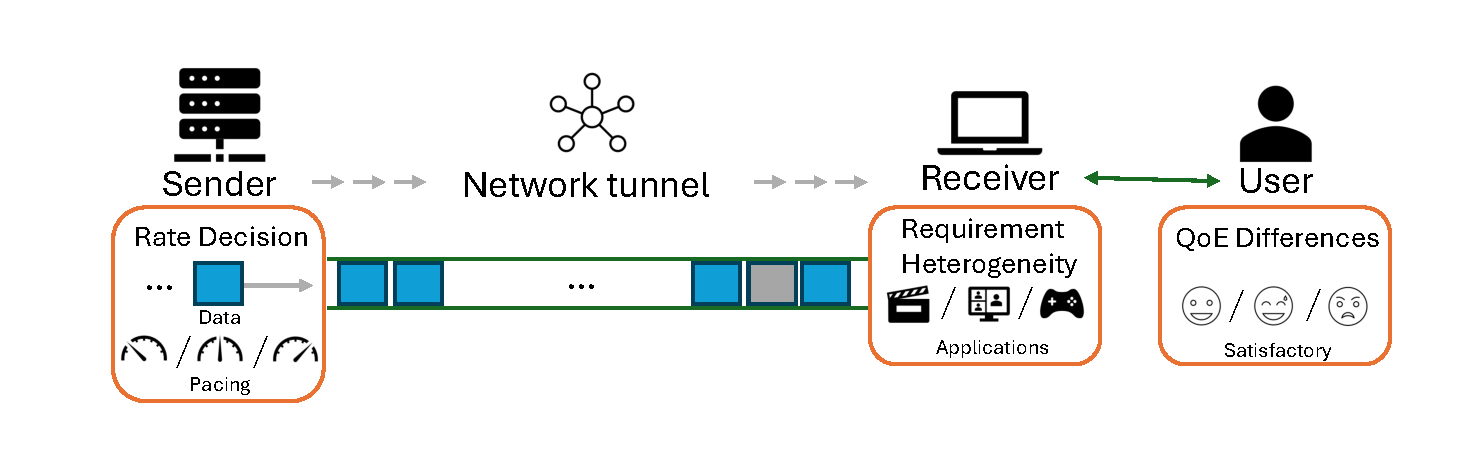
\includegraphics[width=\textwidth]{figures/chap01/system_archi.pdf} 
\caption{网络传输速率控制系统架构示例}
\label{fig:teaser_system_archi}
\end{figure}


随着应用场景种类的增多,服务目标和用户偏好的分化造成了网络媒体应用对网络传输需求的异质性增加。例如流式视频点播的服务目标是在避免视频重新缓冲致使停顿的同时,尽力提升画面清晰度;视频会议直播的服务目标是保证低时延,与面对面交流反应时延的一致;云游戏视频的服务目标是保证用户交互反馈时延与本地游戏的一致性;远程手术需保证网络的稳定和可靠性;360$^{\circ}$视频的服务目标是视点内容的画面高清晰度。利用网络媒体应用对网络传输需求的异质性作出针对性的优化能够降低传输信息冗余,提升同等投入下的服务质量。若忽视服务目标的差异性而提供同质化的控制策略,也将折损用户体验质量(Quality of Experience,QoE)\cite{zhang2019e2e}。因此,网络媒体应用对网络传输需求的异质性已是策略设计中不可忽视的重要问题。

另一方面,传输速率控制策略经过了几十年间研究者的探索和积累,已经形成了庞大的可用策略库。这些策略由于具有差异的设计原理,呈现出对于不同的网络环境适配的差异性。例如,WestWood\cite{casetti2002tcp}被用于在无线网络下工作,POLYCORN\cite{ni2023polycorn}用于连接不稳定的网络下工作,Copa\cite{arun2018copa}用于超低时延环境下工作。传输速率控制策略的性能适配差异性为不同特性的网络环境提供潜在的选择。

然而,现存的传输速率控制策略面对网络传输需求的异质性和网络环境所需的性能适配差异性时,无法提供针对性优化。造成这种不足的原因是这些算法不具备感知应用场景并了解服务目标的能力,以及无法针对异质化的应用场景确定一个可量化的优化目标,为控制算法的针对性优化带来了困难。除此以外,现有的网络传输速率控制工作范式(Paradigm)通常采用固定的策略选择,无法利用上庞大的可用策略库。

% 一张图阐明 策略差异 以及 应用需求差异

在以上背景下,本文旨在设计一个可感知场景异质性的策略及一个新的传输速率控制范式,能够使策略感知具体网络媒体应用对网络传输需求,并根据感知的网络环境特性切换策略,提升传输信息的对用户体验的增益。

\section{研究挑战与内容}
现存的网络传输速率控制策略在面对传输异质化的应用场景时,缺乏对场景和用户偏好的定量感知能力和能利用感知结果的差异化控制策略;网络传输控制工作范式亦存在对所有网络状况和网络特性采用固定的策略选择的缺陷,造成了相同瓶颈网络条件下用户体验的次优。本文认为,用户体验的次优可以通过重新设计一个能够感知场景和用户偏好的策略以及利用上过去几十年累积的庞大的可用策略库来进行体验提升。具体的研究内容如图\ref{fig:final_goal}所示,其主要思想是利用两个环节的异质性和差异性,从两个角度切入优化速率控制模块,提升服务质量。

\begin{figure} [ht]
\centering
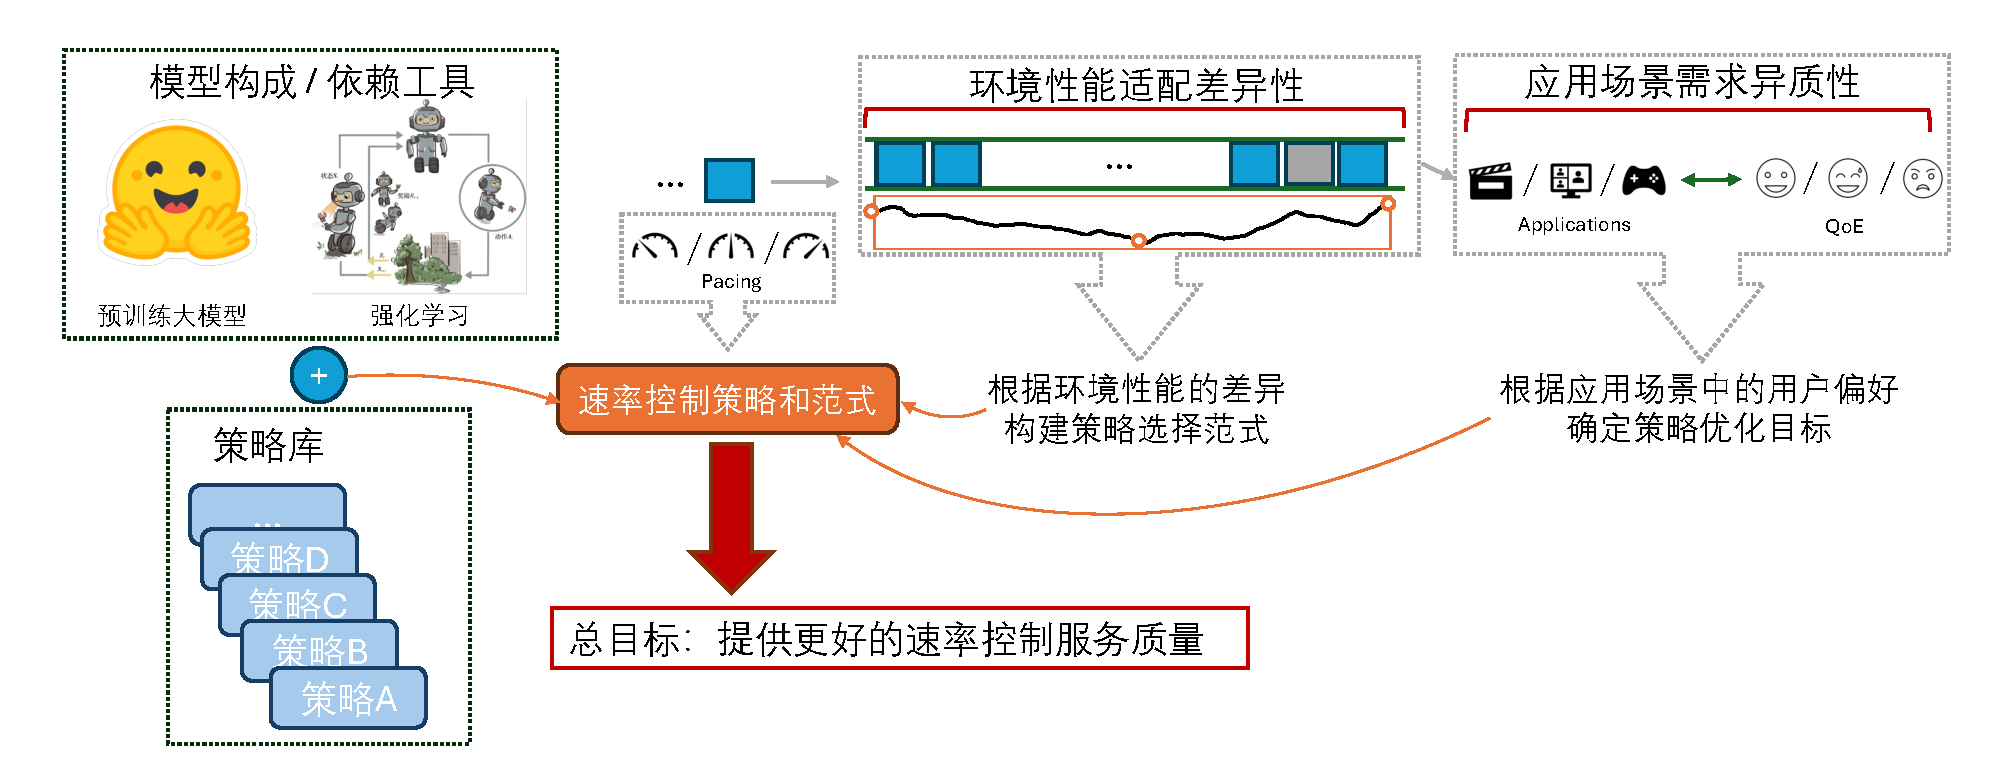
\includegraphics[width=\textwidth]{figures/chap01/final_goal.pdf} 
\caption{研究内容与框架}
\label{fig:final_goal}
\end{figure}


然而,实现服务的提升与速率控制质量改善的总目标需要解决以下挑战:
\begin{itemize}
    \item \textbf{如何根据应用场景中的用户偏好确定策略优化目标:} 网络传输需求的异质性使不同的应用场景有不同的优化目标。尽管根据用户需求能够直观地提供场景的定性分析(例如需要低时延或高吞吐量等),但是定性分析的结果难以作为某一策略的优化目标,需要可量化的方程式才可供算法进行最优解的迭代。然而,确定一个能直接反馈特定场景传输偏好的量化公式,需要对应场景下的用户反馈映射为网络指标的函数表达式。确定用户偏好至策略优化目标函数的映射方式是重要挑战。
    
    \item \textbf{如何设计可对场景感知的传输速率控制算法:} 传输速率控制算法需要具备对应用场景内容感知的能力,并将感知结果作用于算法的工作模式或参数调整上。对应用场景的感知需要依赖可靠的感知指标和能够进行特征提取的感知方法。传输速率控制算法在多影响因素(应用场景变化和网络波动)中,通过与外界环境感知和交互达到优化目标的最优解是一个复杂的决策任务。

    \item \textbf{如何利用累积策略库构建网络任务规划框架:} 现有的网络协议在建立连接后可动态切换策略的能力,因此要实现可切换策略的控制范式需要重定义工作流程,增加对宏观网络运行环境特性的感知,并支持策略库中策略切换。策略库的构建和更新需要范式具备提取策略工作特性和优点的能力。
    
\end{itemize}

本文着重讨论了应用场景下网络传输需求的异质性和策略环境适配的差异性的问题,旨在优化传输信息对用户体验的增益。基于以上挑战,研究内容主要包括以下两个方面:

(1) 用户时延敏感度可感知的场景化传输速率控制算法

针对于网络传输需求的异质性,本文提出“时延敏感度”的概念,并旨在将时延敏感度通过数学方法映射为量化的函数,将此函数作为强化学习速率控制方法的优化目标,训练出不同场景下的最优解。通过开展针对真实用户场景下的评分测试获取用户满意与特定场景下网络指标之间关系的数据,解决上述的第一个挑战;随后设计基于强化学习的传输速率控制算法,使用流式画面内容编码器提供的信息作为场景感知信息,在高度波动的网络环境下结合场景特性和用户敏感性完成传输速率的控制,解决上述第二点挑战。本研究内容提供一种在带宽受限的情况下微调延迟和流式传输质量之间权衡的内容敏感方法。该研究内容的核心理念是在有限的带宽内,根据用户实验确定的延迟影响体验范围,在延迟和流式传输视觉质量之间取得平衡,从而提升用户体验质量(Quality of Experience,QoE)。由于云游戏设计多种场景,本工作在云游戏的多个差异化场景下展开测量和评估。

(2) 具备策略库的网络任务规划范式设计

针对于策略环境适配的差异性,本文旨在提出一个新范式,能够将过去网络控制策略选择范式中固定和对所有连接统一的固定策略,不会灵活更换的设计方案作出更新化迭代。为了将过去数几十年的算法构成可供备选的策略库,需要学习到策略所适配的网络特性和算法特点,形成可以根据网络环境特性作出最佳选择的范式。为了实现对历史策略的学习,构建策略切换的流程和作出选择决策,本研究内容包括对网络传输通信的控制协议流程进行重新设计,使其支持控制策略切换;网络策略的选择则需要感知网络特性,选择合适的策略,该研究内容解决了上述第三点挑战。近年来大模型可以作出决策的能力涌现,包括对环境理解的能力、推理和决策能力。因此本研究内容将使用预训练大模型进行网络控制策略选择范式设计。

\section{研究主要贡献}
本文的主要贡献点如下:

(1) 设计了一个可对场景中用户偏好感知的云游戏下实时通信传输速率控制算法。该算法首先通过对用户开展主观打分实验获得平均意见分数(Mean Opinion Score,MOS),确定了不同的应用场景下的三种敏感度类型,并使用了最小二乘估计(Least Square Estimation,LSE) 的数学方法估计拟合高、中、低敏感度的延迟感知敏感度曲线。算法将敏感度曲线作为奖励函数,使用Actor-Critic 架构强化学习速率控制算法为不同的时延敏感度场景量身定制,有助于实现延迟和视觉质量之间的更好平衡,从而使 QoE 提高高达 16.7\%。为了减少对于用户敏感度主观评分的依赖,此算法还使用来自视频流的信息,即时间感知信息 (Temporal perceptual Information,TI) 和空间感知信息 (Spatial perceptual Information,SI) 对游戏的敏感度进行分类,准确率达到 89\%。

(2) 重构了具备累积策略的网络任务策略规划范式构。该算法通过对现有的传输速率控制范式进行流程重定义,改变了过往在网络传输控制中固定一成不变的策略,增加了一个连接建立前的网络特性探测机制,使用预训练大模型(Pretrained Language Model,PLM)的感知与规划能力,为差异化的网络环境和连接流提供选用不同的策略的潜在可能性;通过在模拟环境下采集多个已有策略的工作模式和工作流程确定了方法适配的网络环境,并对预训练大模型(LLaMA)增加时序感知的嵌入(Embedding)模块,使用低秩矩阵分解(Low-Rank Adaptation,LoRA)的方法对大模型的输出进行微调和对齐,提升大模型选择策略和参数的有效性和成功率。该方法成功建立一个稳定和不易出错,且有效地利用上策略差异性提升网络传输速率控制质量的范式,超越了传统范式中单一算法在波动的网络环境中的运行性能。


\section{论文组织结构}
本文一共包含五个章节,图\ref{fig:arrange}展示了每个章节的内容。第二章概述了现有的网络传输速率控制策略在解决传输需求的异质性和策略环境适配的差异性的相关工作,包括对现有速率控制策略的总结与分类、对于传输需求的异质性的研究工作总结和利用策略环境适配的差异性的范式总结,以及方法所涉及强化学习框架的介绍。
第三章主要介绍场景时延敏感度可感知的传输速率控制,包括对用户偏好的量化感知方法和强化学习速率控制方法的设计。
第四章主要介绍具备策略库的⽹络任务规划范式设计,包括对范式工作流程的设计方法和对应的网络控制流程训练时大模型的微调对齐方法。
第五章对本文的研究内容进行总结,并对未来的研究方向作出展望。

\begin{figure} [ht]
\centering
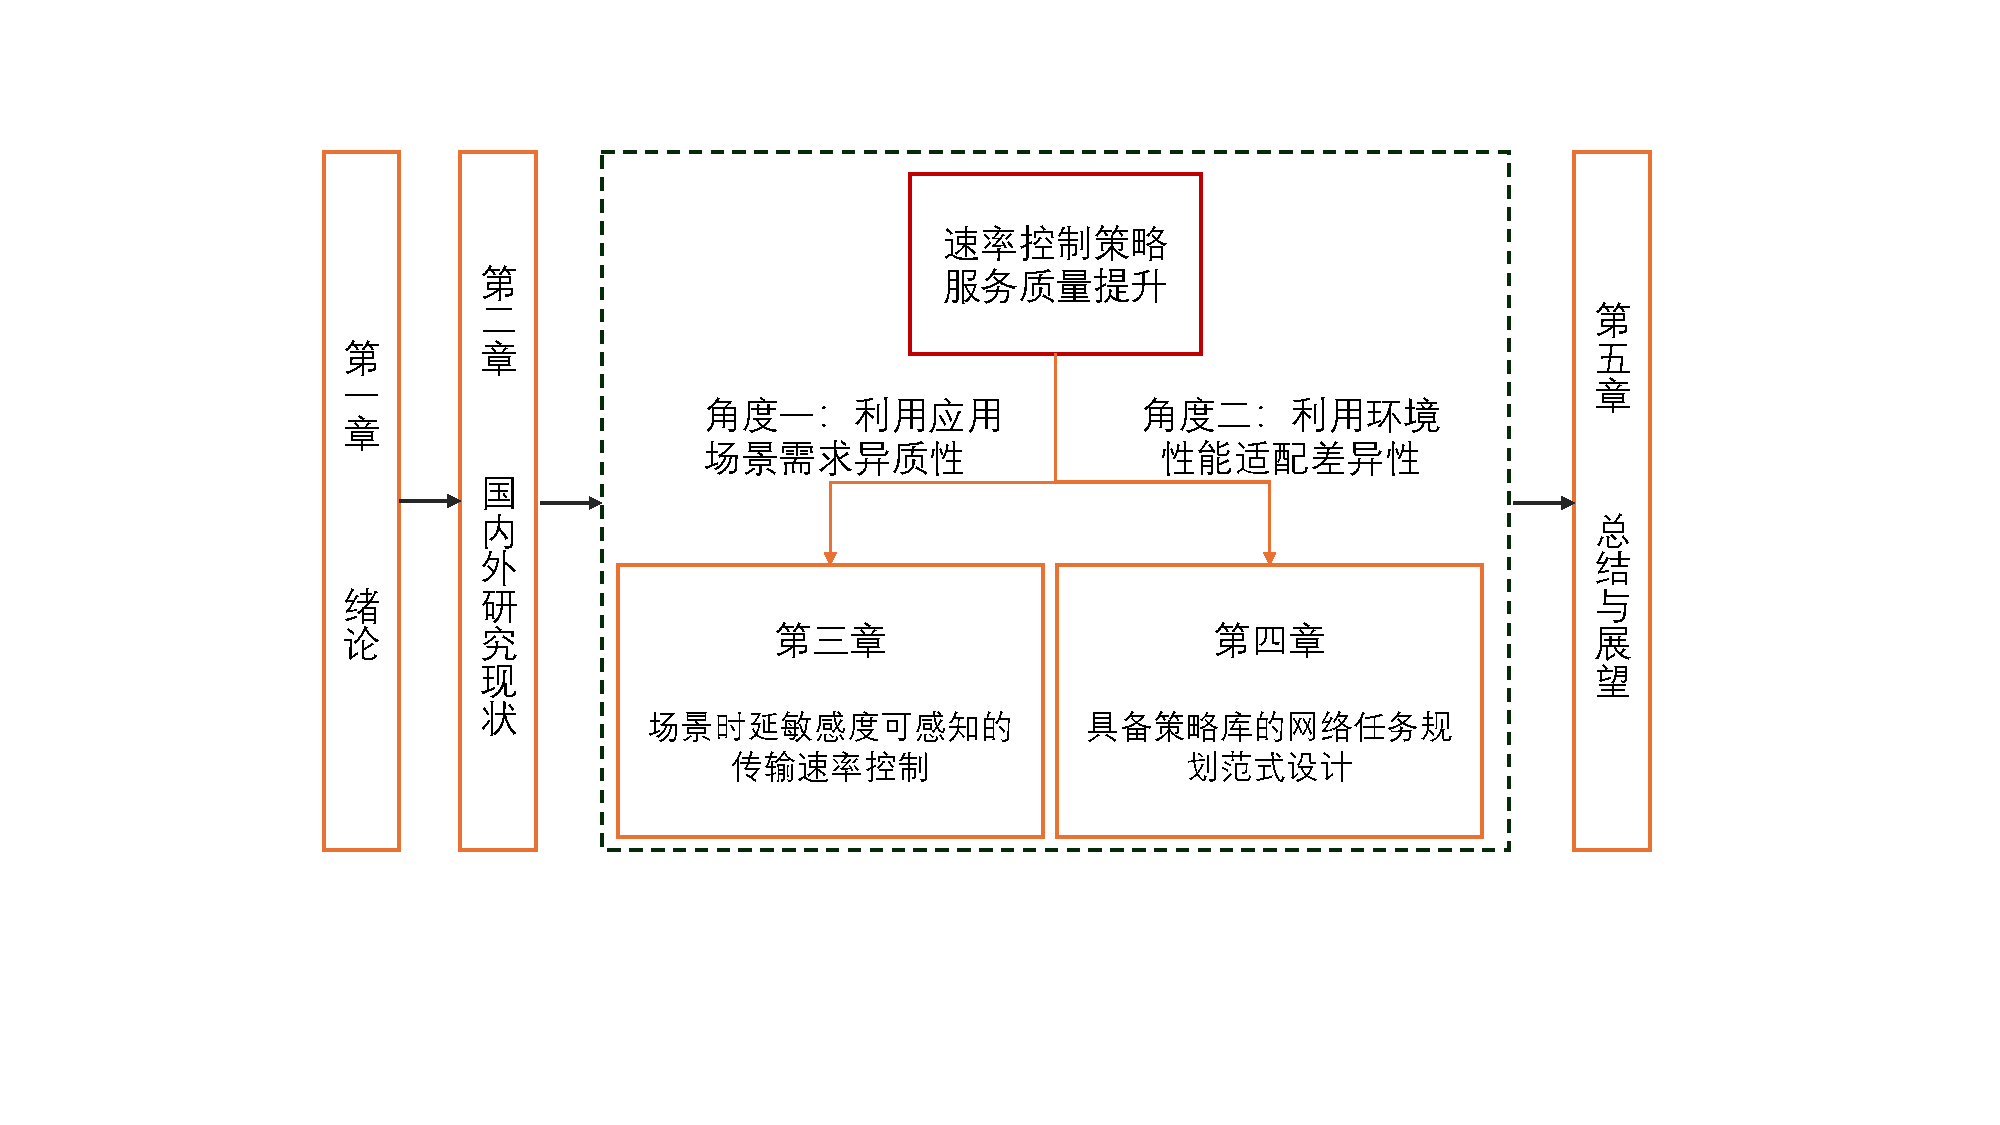
\includegraphics[width=0.8\textwidth]{figures/chap01/arrange.pdf} 
\caption{本文各章内容安排与结构}
\label{fig:arrange}
\end{figure}

% !TeX root = ../thuthesis-example.tex

\chapter{国内外研究现状}
传输速率控制策略作为网络应用领域重要的决策任务,已经在多年的研究下累积了许多重要工作。本章节将根据研究挑战,将相关工作分类为针对应用场景需求异质性的研究和针对策略环境性能适配差异性的策略研究两个方面分别介绍传输速率控制策略的研究发展,为传输速率控制策略的问题分析和方法研究提供基础。此外,本章还简要介绍了有关强化学习背景的相关工作。

\section{针对应用场景需求异质性的研究}
应用场景需求异质性是指由于媒体系统的服务目标和对象不同所带来的差异。通过利用这种异质性,可以有效地提升服务目标的用户体验质量。目前有很多工作针对定义用户体验质量展开研究;部分工作尝试揭露某特定应用下的独有差异性,为算法优化提供了有效的重要参考指标。

\subsection{用户体验质量的研究与定义}
用户体验质量(Quality of Experience,QoE)的研究是实时通信系统中用于评估服务质量的重要一环。它为如何设计系统、如何分析系统性能和如何评价系统实现效果带来指导性作用。根据林闯\cite{林闯2012用户体验质量}等人的研究,用户体验质量可以被定义为在用户角度对于整个服务质量的评价,包括了主观因素和客观服务质量指标(Quality of Service,QoS);QoE的影响因素也可根据该研究分为环境、用户和服务三类,如图\ref{fig:Qoedef}所示。

\begin{figure} [ht]
\centering
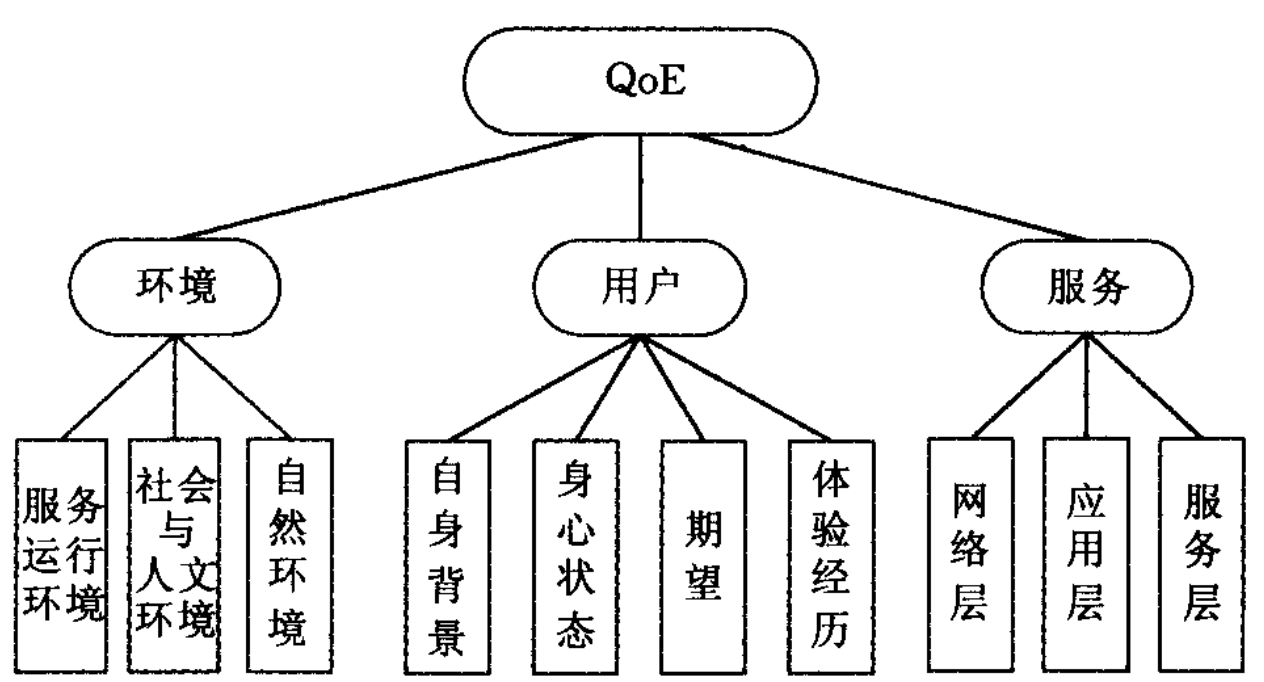
\includegraphics[width=0.7\textwidth]{figures/chap02/QoE.png} 
\caption{QoE中包含的可考虑因素列举\cite{林闯2012用户体验质量}}
\label{fig:Qoedef}
\end{figure}

新的应用类型因为提供服务需求的改变,用户主观的感知质量会因此而产生影响。同时,用户体验质量能够作为最终优化目标,指导系统优化工作。当前已经有多种类型的,从不同的场景与角度出发的QoE评判方式。例如,内容服务提供商可能将使用时长作为关键的QoE指标\cite{CTR洞察},因为高用户留存率可以带来高经济收益;而对于个人用户,当遇到系统抖动时,呈现内容品质降级的过渡策略(例如画面跳过、画面预测、自适应比特率或重新加载)可能会对于用户感受质量造成非常大的影响。

一部分工作会试图在模拟网络拓补下的开展用户主观评分,获取直接的用户真实反馈。这类工作在局域网的拓扑上利用网络模拟器(如NetEm\cite{hemminger2005network}, Mahimahi\cite{netravali2015mahimahi}, ns-3\cite{henderson2008network}或其他工具)模拟真实的网络可能遇到的环境,并通过用户五分制打分(MOS)\cite{林闯2012用户体验质量}的方式衡量某些因素对用户体验质量的影响。目前已有在云游戏、视频业务和其他类型的实时服务商开展此类研究的工作\cite{jarschel2011evaluation,ahmad2023significance,zadtootaghaj2018modeling,zhang2019e2e,lindstrom2020cloud}。工作引入了多种因素的端到端网络,例如高延迟、抖动、丢包、带宽控制和资源分配,以及视频特性中的码率等因素,衡量每个因素的影响多少。参与者会被要求在一个阶段后对前述感受进行五分制的打分。

另一种方式是识别重要指标并建立一个质量预测模型给出打分。这类工作通过大规模的数据测量,尝试识别新的应用中特有的能够反映用户QoE的指标,并根据这些指标建立预测模型。这一类工作包括\cite{balachandran2013developing,cheng2023rebuffering,zhu2022eyeqoe},分别应用于视频观看、短视频点播和VR全景视频。用于评估QoE的指标在建立预测模型时可能会有多个,包括实时通信系统中的诸如时延、抖动通用的指标,到用户退出率、眼动位置坐标等应用特有数据,这些数据共同作为模型的输入,构成最后的QoE预测模型。

还有一部分工作着重研究了画质和码率切换对于用户体验带来的负面影响的具体衡量方法。\cite{slivar2016cloud,jamshidi2022deep,utke2022ndnetgaming}中通过将画面灰度的峰值信噪比(Peak Signal-to-noise ratio,PSNR)或视频多方法评估融合(Video Multimethod Assessment Fusion, VMAF)指标值区间映射入各自的长短时记忆模型(Long Short-Term Memory,LSTM),获得以秒为粒度的预测用户质量数据。
\cite{mao2017neural,huang2019comyco,nathan2019end}在对于各自的模型进行评估时使用式\eqref{equation-qoe}进行QoE中品质降级的过渡策略(画面跳过、画面预测、自适应比特率或重新加载)带来的影响的量化衡量:
\begin{equation}
    QoE = \sum_{n=1}^{N}q(R_n) - \mu \sum_{n=1}^{N}q(T_n) - \sum_{n=1}^{N-1}\lvert q(R_{n+1})-q(R_n) \rvert,
\label{equation-qoe}
\end{equation}

其中, $N$ 代表视频块的数量,$R_n$ 代表第 $n$ 个视频块的比特率,$T_n$ 代表第 $n$ 个视频块重加载的时间,最后一项代表比特率切换的影响,亦被称作为流畅度。 $\mu$ 则是经验值罚项。


\subsection{特定应用需求差异性分析工作}
E2E\cite{zhang2019e2e}对互联网上流量吞吐提出了大型范式,涵盖了所有涉及用户参与的连接请求,其核心思想在在于挖掘用户对于应用需求的QoE异质性。对于云游戏、视频会议、360$^{\circ}$视频等不同种类的应用,现有的工作对它们展开了针对性的探索。ClayPool等人尝试描述网络游戏中玩家对于其操作响应和画面变化延迟的敏感性\cite{claypool2006latency,claypool2010latency},使用网络时延对于用户表现分数的影响说明了游戏内容对时延要求差异的存在和定性,并给出了要求的极端下限阈值。EyeQoE\cite{zhu2022eyeqoe}在VR设备的使用过程中和360$^{\circ}$视频的播放对用户的眼球运动进行追踪,对具体的眼球运动分类并捕捉运动模式,以预测其运动轨迹和感知质量。Michael等人尝试开展对于用户的主观测试\cite{jarschel2011evaluation},并发掘了游戏节奏是有差异性的,这种差异性造成了对网络时延控制、丢包控制等优先性的偏好不同。Cheng等人在大型短视频服务提供商的数据集上进行了广泛的用户行为研究\cite{cheng2023rebuffering}。测量数据表明,不同的视频流内容虽然在遇到卡顿时会让用户不满,进而增加用户的提前退出率,但是它们的概率是有所不同的,体现出不同视频流卡顿对QoE影响的差异性。


\section{环境性能适配差异性的策略研究}
环境性能适配差异性是指由于所处网络的环境所固有的属性有所不同带来的差异。这种差异性通常是由于物理层的链路特性、网络使用所处的环境、网络应用的差异,或与不同时段带宽链路的利用率等有直接相关性。针对这样的差异性进行研究,可以针对于网络的特性更好地做出相适配的决策,进而提供更可靠的网络传输保障和更好的服务质量。目前有大量工作针对于此差异性展开了深入和广泛的研究。

\subsection{适用于差异化环境性能的速率控制算法研究}
速率控制是一个重要的传输速率控制策略,工作于网络的传输层,在实践应用时有时会交由应用层完成其功能。它的目的是为了保证传输的可靠性和效率。一个常见的网络点对点连接可以抽象为一个如图\ref{fig:sending} \cite{author2024performance}所示的结构:发送器和接收器对应两条不同的路由,而在链路上会遇到瓶颈带宽。发送器需要控制发送的速率以确保一定的带宽利用率才能保证传输效率,并避免其过大造成的发送失败。“速率控制”通常被理解为可靠传输控制协议(即TCP协议)中发送端根据网络状况和接收窗口的情况实行发送包的控制,或是应用层根据接收缓冲区的状况进行的码率发送选择。在TCP拥塞协议的约定下,接收方必须对于每个接收到的包回应一个ACK信号(部分情况下,多个包可以使用ACK聚合回应一次),发送方也需要等待发送的前序包确认收到后再发送后续包。但在实时通信系统中,使用可靠传输协议的等待ACK信号会大幅降低系统的实时性,因此多数系统和应用在传输层使用了数据报的方式进行传输,而将可靠传输的任务交由应用层完成,例如QUIC\cite{langley2017quic}协议。在这种情况下,协议根据流式媒体内容的特性针对性进行拥塞控制。同时由于通信系统中网络时延和网络抖动带来的负面影响占据了总时延比重的主要部分\cite{yuan2022understanding},大量发送速率控制和流量管控工作集中于这一环节,针对于不同的环境性能进行改善。系统整体的性能亦随速率控制算法的进步而得到改善。

\begin{figure} [ht]
\centering
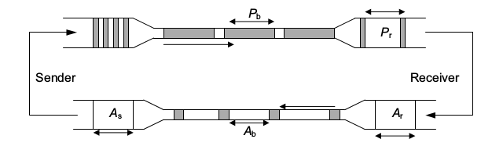
\includegraphics[width=0.8\textwidth]{figures/chap02/sending.png} 
\caption{速率控制的工作环境和其目的\cite{author2024performance}}
\label{fig:sending}
\end{figure}


速率控制通常可以根据其探测所依赖的关键信息进行区分,例如基于网络丢包(loss-based)信号、基于时间延迟大小(delay-based)信号、或是基于时延-带宽积(Bandwidth-Delay Product)信号等。除外,速率控制还可依照建立的不同的理论进行区分,例如延迟排队理论建模、固定规则、启发式算法、预训练监督学习模型方法、强化学习和基于用户感知的方法等。本章节将结合多个方面,对现有的速率控制算法展开。本章节还将会从拥塞控制的特性和适配环境角度切入进行总结。

基于网络丢包(loss-based)的拥塞控制主要探测超时未收到确认信号的包数量。根据某一时间段内的丢包率推断出网络遇到了多大程度的拥塞,并及时采取措施缓解拥塞。Tahoe\cite{jasim2018old}, Reno\cite{yang2000general}和New Reno\cite{fall1996simulation}是经典的基于网络丢包的速率控制算法,它们都使用了慢启动(从低阈值开始指数增长拥塞窗口)、拥塞避免(临近预测的拥塞阈值时,线性增长拥塞窗口)、快重传(丢包后乘法降低至低值后再上升)的方式进行拥塞控制。它们三者的区别是Reno相比于Tahoe多出了快恢复算法,避免在丢包后回到慢启动阶段,降低传输效率;New Reno则改进了快恢复机制,避免单次拥塞的发生被认为是多次。根据其拥塞方法的控制原理,它们适用于相对时延不那么敏感的任务和网络缓冲区较大的任务,以及要求获得更高的吞吐量的任务。

BIC-TCP\cite{xu2004binary}和Cubic\cite{ha2008cubic}是另外两个相似的基于网络丢包的速率控制,使用窗口增长函数完成窗口的估测,Cubic使用一个奇数阶多项式修正窗口增长函数,增加了窗口增长的稳定性,避免过激带来丢包。Cubic也是目前Linux内核中默认采用的拥塞控制算法。相比于Reno,Cubic类的算法能够更快地恢复拥塞窗口。上述的Reno、Cubic都是基于一个固定规则的方法,具有极佳的稳定性。

基于测量时延(delay-based)的拥塞控制主要基于探测包发送到到达的时间或其计算后的元素。通常来说,从发送端向接收端的发送路径和从接收端向发送端的发送路径应被视作两条异质化的、无相关性的链路,这是因为它们经过的路由可能不同,或即使相同网络状况也有所差异,网络带宽有所不同。但是,由于测量手法限制,实际测量时会根据往返时延(Round-Trip Time,RTT)的一半作为时延的估测使用,判断网络的状况。还有部分算法会使用往返时延对单位时间$T$的微分($\frac{dRTT}{dT}$),即包到达时间间隔的差异作为衡量标准。TCP Vegas\cite{brakmo1994tcp}使用连接中数据包的RTT决定发送速率和探测带宽。Google于2015年提出的BBR\cite{cardwell2016bbr}亦使用了这样的思想。作者认为,由于缓存技术的发展,网络这一本该即用即走的链路因为路由设备和中继设备的缓存装置使之有了存储的功能。由于网络设备处理能力有限,在应用发送包不断增加时,首先到达处理能力瓶颈。此时发送出的包容量为一个时延带宽积(BDP)。此时如果发送速率继续上升,会在网络存在的缓冲区中存储。此时会导致发送包处理的队列,造成ACK回复的时间变长,此时体现为测量到的往返时延(RTT)增加;直至网络缓冲区也被填满,此时就会产生丢包。BBR使用固定的时段探测带宽,并根据结果对于发送速率进行乘以固定因子的挑战,不断自适应网络状况。这一类方法也使用了一些固定的规则,带来可靠的同时适用于需要较低时延,但不存在较多竞争的任务。

而Copa\cite{arun2018copa}是一种默认工作在以传输时延作为探测信号的发送速率控制方法,保证低时延应用的传输;然而,在探测到其他丢包流竞争的时候,Copa会切换到以丢包为探测信号的工作模式中,以便在多流竞争中取得相对的公平性。这是由于当基于丢包控制算法与基于时延为信号的控制算法在一个瓶颈带宽时,时延瓶颈通常会先于丢包发生,造成算法竞争的不公平。Venkat Arun等人在工作\cite{arun2022starvation}中揭露了当前所有基于测量时延的拥塞控制算法中存在的多流竞争导致的部分算法的饥饿的现象,通过一个网络模型复现了多个前述算法在竞争中存在的缺陷,并给出了饥饿产生和拥塞算法收敛的推导,揭示了问题的本质。Copa对于网络的拥塞控制服务基于的原理是排队论中的 M/M/1 模型,建立在将包到达时间视为泊松过程(Poisson process)这一假设上对于发送速率进行优化,进而使网络利用率最高。这种算法能够兼顾低时延与公平性,适用于多流竞争情况下的低时延保障场景与任务。类似地,WebRTC中采用的GCC\cite{carlucci2016analysis}使用了混合丢包与时延策略的算法同时借助两种信息进行判断。延迟间隔经过多个滤波器后得到一个发送速率,同时丢包探测器同步进行丢包检测,同样给出一个发送速率,选择两者较小者实行。

SQP\cite{ray2022sqp}使用了贴近于视频帧的发送策略,即以帧为单位,单次发送时将一帧的多个包在短时间内发出,并根据收到的ACK时间戳估测带宽的使用情况,恰好用作带宽探测。SQP根据每帧的第一个包的发送时刻与上一帧最后一个包的接收时刻之间的差值作出带宽过度/不足利用的估计,并根据该时间间隔完成发送速率的调整。这种方法适用于低时延视频传输的环境。

PCC-Allegro\cite{dong2015pcc}和PCC-Vivace\cite{dong2018pcc}将时间切分为检测间隔(Monitor Intervals),使用一个效用函数完成拥塞控制,内包含对于时间间隔与丢包情况的权重估计。而它们的区别在于PCC-Allegro会使用探测性决策方法决策发送速率,是基于传统方法的策略;而PCC-Vivace则使用了在线学习,通过梯度在线优化算法完成发送速率的调整。PCC-Expr则是另外一个PCC系列的变种,旨在提高通过率和延迟控制之间的平衡,特别是在需要极低延迟的环境中。

得益于强化学习在决策类任务的优异性能表现\cite{mnih2013playing},使用强化学习的速率控制方法也在近年来出现和发展。Orca\cite{abbasloo2020classic}便是一个基于强化学习的拥塞控制方法,他指出了当前纯学习型拥塞控制设计的不足,并表明选择深度强化学习能够从原始数据中提取出高度有效的信息,并与环境互动,逐步做出决策。Orca通过将含有吞吐量、时延和带宽利用情况的指标量化为一个奖励值作为强化学习的学习目标,并使用了精细设计的模块,成功将强化学习应用于拥塞控制任务中,在全球范围的测试平台上部署的Orca实现了良好的效果。Aurora\cite{jay2019deep}使用了类似的强化学习方式实现了拥塞控制,并尽可能保障了多流竞争之间的公平性与安全性。这类方法使用网络变化大、连接时间长,需要时间适应的独特特性网络,但对于部署算法的要求较高。 R3Net\cite{fang2019reinforcement}使用了相同的方法但设计了差异化的模型以便更好地提取出网络信息,服务于实时通信系统中的发送速率控制或是传输层的拥塞控制。

随着强化学习的发展,强化学习被用于速率控制的情况越来越多,尤其是RTC系统中的实时速率控制。为此,微软推出了一个仿真平台OpenNetlab\cite{eo2022opennetlab},它将一个RTC仿真模拟器封装,并抽离出对接强化学习算法的接口,还提供真实部署在各地的服务器用于测试性能。ReCoCo\cite{markudova2023recoco} 是使用该仿真平台构建的,专用于超低时延的实时通信任务的基于强化学习的发送速率控制模型。


亦有一部分工作基于场景总结后的用户感知特性完成算法控制的优化。例如,PACC\cite{peng2023pacc}是使用了卷积神经网络(Convolutional Nerual Network,CNN)构建画面的传感器模块,从而有选择地高质量传输更重要的部分。这样的策略与上节的QoE形成更紧密的耦合。


除此以外,环境性能适配差异性还体现在更细粒度的具体场景上。比如,在高速铁路上,由于快速的移动,基站部署的稀缺,会导致收发消息的链路可靠性衰减。针对于这样与常规环境不同的差异性,POLYCORN\cite{ni2023polycorn}和Cellfusion\cite{ni2023cellfusion}使用了多径改善了户外或高速铁路上移动时的信道质量。通过不同运营商提供的两个链路和自适应的补偿机制完成了发送。这一类针对不同应用而采用多链路方式弥补的工作也有很多,比如针对于视频会议的Converge\cite{dhawaskar2023converge}和Twinstar\cite{wang2023twinstar}。

\subsection{适用于不同场景的自适应码率算法研究}
自适应码率也是发送速率控制算法中的重要一部分。相较于工作在传输层的拥塞控制类型的发送速率控制任务,它有的独特特点是更粗粒度的决策和有限的决策选择。自适应码率流式传输算法的工作原理如图\ref{fig:abrteaser}所示。

\begin{figure} [ht]
\centering
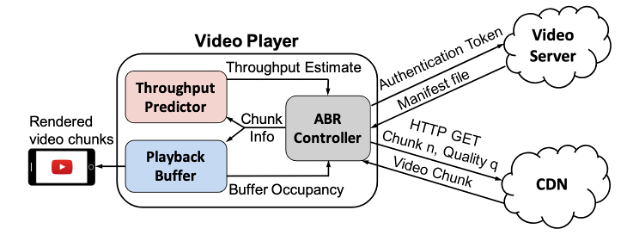
\includegraphics[width=0.75\textwidth]{figures/chap02/abrteaser.png} 
\caption{自适应码率流式传输系统的工作原理\cite{mao2017neural}}
\label{fig:abrteaser}
\end{figure}


自适应码率流式传输系统根据网络的实时带宽情况动态选择合适的码率来传输视频内容。每个视频被预先转码为多个不同码率的片段(chunk),每个片段代表视频中的一个时间段,大约几秒。在播放过程中,系统根据当前网络状况和客户端的缓存状态,选择一个合适的码率进行下载。当网络带宽较好时,系统会选择较高的码率以提供更高质量的视频体验;而在网络带宽受限时,系统则会选择较低的码率以避免视频卡顿和缓冲现象。自适应码率算法通过定期监测网络带宽和视频播放状态,调整发送码率以确保视频流畅播放。自适应码率流式传输算法通常基于反馈控制机制,如图\ref{fig:abrteaser}中的控制器所示(ABR Controller)。客户端通过定期发送网络带宽反馈给服务器,服务器根据这些反馈信息决定下一个时间段内应选择的码率。常见的自适应码率算法包括基于带宽估计的算法、基于延迟的算法以及混合算法等。每种算法都有其优缺点,需要根据具体应用场景进行差异性的选择。

经典的自适应码率流式传输算法有模型预测控制方法(Model Predictive Control,MPC)\cite{yin2015control}方法,一种传统的基于规则的方法。这种方法利用动态规划的方式,将吞吐量估计和关于缓冲区占用的观测信息用于选择在未来一段时间内最大化给定 QoE(用户体验质量)指标的码率。除外,基于缓冲区的自适应码率算法(Buffer-Based Algorithm,BBA)\cite{huang2014buffer}基于客户端的缓冲区占用情况来调整视频的码率,而不是依赖于复杂的容量估计。通过这种方法,能够在不依赖复杂的容量预测的情况下,减少 10\% 到 20\% 的重缓冲率(rebuffer rate)。BOLA(Buffer Occupancy based Lyapunov Algorithm)\cite{spiteri2020bola}是一种基于缓存占用率的自适应码率算法,能够通过控制缓存的上下限来避免缓冲过多或过少,从而确保视频的流畅播放。以上三种方法都是较为传统的,基于固定规则的算法,具有较好的稳定性,但可能缺乏灵活性。

Pensieve\cite{mao2017neural}是使用强化学习完成自适应码率任务的代表。该算法使用了一个可并行的演员-评论家(Actor-Critic,加并行后表示为A3C)进行码率选择的决策。它能够自适应调整策略,学习不同网络条件下的最佳行为,从而实现流媒体传输的最优体验。Genet\cite{xia2022genet}是在Pensive基础上进一步改良的自适应码率任务,并扩展到了更多发送速率控制相关的人物上。它的改良主要是利用了课程学习的方式,让强化学习的过程从较简单的内容逐渐转向复杂的内容。



\subsection{差异性对比与工作范式研究}
在速率控制算法的发展基础上,一个庞大的历史可用库得以累积。为了统计、分析这些速率控制方法的性能以及站在更大的角度审视它们,性能对比的工作和范式规划的工作被提出。

近年来预训练大模型的出现为这一类任务提供了新的思路。得益于大模型强大的推理和决策能力,NetLLM\cite{wu2024netllm}提出了“一个模型适用所有网络任务”,亦包括了自适应码率的任务。为了适配码率的时序数据,NetLLM使用了一个多模态编码器,将网络状态时序信息编码进大模型的嵌入层;经过大模型的前向传播后限定输出头以准确地选择最终的码率。由于大模型丰富的经验和知识,NetLLM在实验中取得了优异的表现,为速率控制任务提供了崭新的思路。同样使用预训练大模型的还有LLM-ABR\cite{he2024llm},但采取了不同的思路。LLM-ABR选择让大模型生成出可用的ABR策略,并通过一系列检测和性能测试后使用,进而构建了一个策略创建范式。Nada\cite{he2024designing} 在LLM-ABR基础上进一步改进,扩展到更多网络任务上。


除此以外,许多性能对比的工作为海量的拥塞控制、自适应码率算法提供了真实的部署环境和分布在全球各地的测试平台。Pantheon\cite{yan2018pantheon}和ccBench\cite{abbasloo2023internet}是对于已有算法的部署和测试,提供了一个强大的、真实的、全面的测试平台。Puffer\cite{yan2020learning}则是ABR算法的性能测试平台。部分拥塞控制算法的性能测试的结果和自适应码率的性能测试结果如图\ref{fig-mea-ccabr}所示。

\begin{figure}[ht]
\centering
\begin{subfigure}[t]{0.49\linewidth}
  \centering
  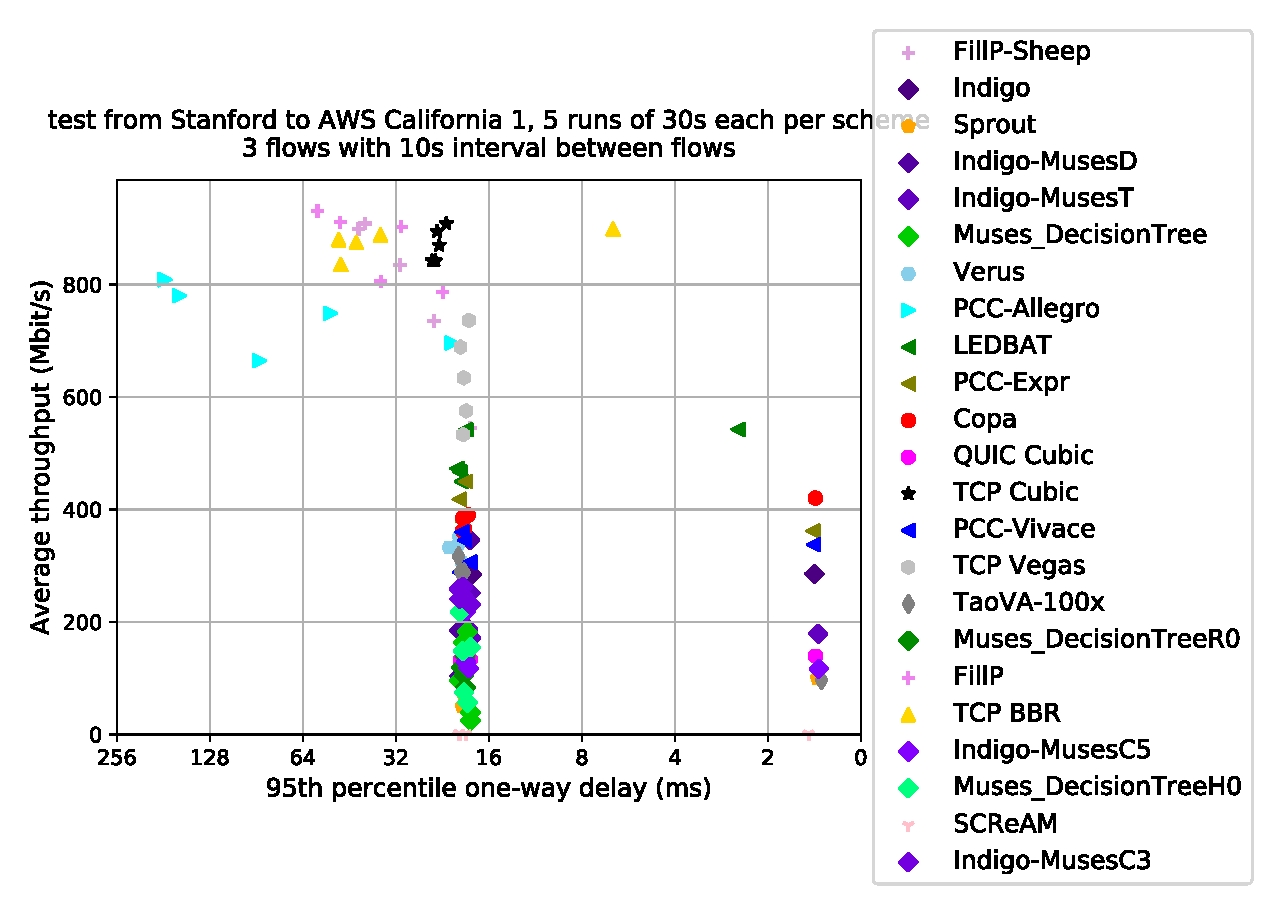
\includegraphics[width=\linewidth]{figures/chap02/measument-ccabr/cc.pdf}
  \caption{拥塞控制算法性能评测}
  \label{fig-measument-ccabr-cc}
\end{subfigure}%
\begin{subfigure}[t]{0.49\linewidth}
  \centering
  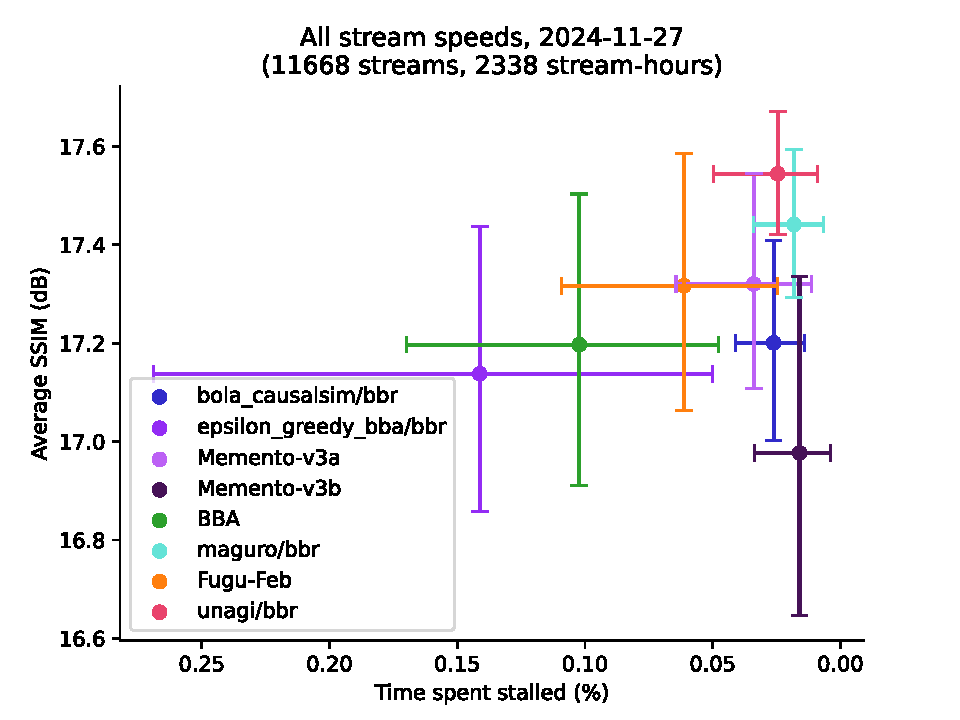
\includegraphics[width=\linewidth]{figures/chap02/measument-ccabr/abr.pdf}
  \caption{自适应码率算法性能评测}
  \label{fig-measument-ccabr-abr}
\end{subfigure}

\caption{Pantheon\cite{yan2018pantheon}和Puffer\cite{yan2020learning}的性能测量结果}
\label{fig-mea-ccabr}
\end{figure}


适配用户需求异质性和网络环境差异性的网络范式也在强化学习蓬勃发展后涌现。E2E \cite{zhang2019e2e}是第一个能够充分利用用户异质性来优化服务器资源分配的系统范式,包括各类发送速率控制算法和场景。E2E系统通过考虑不同用户对服务器端延迟的敏感性来调整资源分配,从而优化整体的QoE。Sage\cite{yen2023computers} 则将过去几十年来的所有拥塞算法的工作模式和行为通过强化学习的方式迁移到它自身身上,构建了拥有所有拥塞控制特性的一个强大的拥塞控制算法。

\section{强化学习领域框架概述}
\subsection{强化学习的基本概念和定义}
强化学习(Reinforcement learning,RL)是一种人工智能范式,涉及智能体(Agent)与环境(Environment)之间的交互,目的是最大化奖励函数 \cite{mnih2015human}。智能体与环境之间持续交互,在此框架下逐步学习,最终习得最优决策策略。

在强化学习中,所有环境中可能观察到的结果形成状态空间 $\mathcal{S}$,它描述了智能体在任一时间点可能观察到的环境状态信息。智能体维护一个策略 $\pi$,该策略定义了智能体在给定状态下采取不同动作的概率分布。智能体根据环境当前状态 $s_t$ 在每个离散时间步 $t$ 决定采取一个动作 $a_t$。所有可以执行的动作构成动作空间 $\mathcal{A}$。一旦环境接收到智能体的动作 $a_t$,它会生成一个奖励信号 $r_t$ 并转移到新的状态 $s_{t+1}$。这个过程不断重复,最终学习到一个策略 $\pi(\mathcal{A}|\mathcal{S})$,该策略最大化奖励的折现总和,这个折现总和用回报 $R_t$ 表示,如式\eqref{eq:rl-reward}所示:
\begin{equation}
\begin{aligned}
    R_t = \sum_{i=t}^{T}\gamma^{i-t}r(s_i,a_i) = r_t + \gamma r_{t+1} + ... + \gamma^{T-t}r_T,
\end{aligned}
\label{eq:rl-reward}
\end{equation}
其中,$\gamma$ 是折扣因子,用于确定短期奖励的优先级。折扣因子 $\gamma$ 的值通常在 $[0, 1]$ 范围内,越接近 1,表示智能体更重视长期回报;而接近 0 时,智能体则更关注近期的回报。在强化学习中,$\gamma$ 调整了未来奖励对当前决策的影响程度。通过合理选择 $\gamma$ 的值,可以平衡探索短期和长期回报之间的关系,帮助智能体制定合适的策略。

强化学习通过学习找到一个最优策略 $\pi_\phi$,其参数为 $\phi$,该策略最大化期望回报。具体来说,强化学习的目标是通过调整策略的参数 $\phi$,使得期望回报(即长期奖励的总和)达到最大。这个过程通常通过优化式\eqref{eq:rl-Jtheta}所示的目标函数来实现:
\begin{equation}
\begin{aligned}
    J(\phi) = \mathbb{E}_{s_i \sim p_\pi, a_i \sim \pi}[R_0].
\end{aligned}
\label{eq:rl-Jtheta}
\end{equation} 

\subsection{强化学习Actor-Critic架构}
在演员-评论家(Actor-Critic)架构中,包含两个网络:演员网络(Actor)和评论家网络(Critic)。演员网络学习最优的策略函数 $\pi_\phi(\mathcal{A}|\mathcal{S})$,旨在学习一个能够生成高奖励并与环境互动的策略。演员使用深度确定性策略梯度(Deep Deterministic Policy Gradient,DDPG)算法 \cite{silver2014deterministic} 来更新策略梯度。具体地,DDPG 是一种适用于连续动作空间的强化学习算法,通过策略梯度更新算法来改进策略,如式\eqref{eq:rl-nablaphi}所示:
\begin{equation}
\begin{aligned}
    \nabla_\phi J(\phi)=\mathbb{E}_{s\sim p_\pi}\left[\nabla_aQ^{\pi}(s,a)|_{a=\pi(s)}\nabla_\phi\pi_\phi(s)\right].
\end{aligned}
\label{eq:rl-nablaphi}
\end{equation} 

评论家网络(Critic network)估计当前策略的价值函数,评估演员(Actor)网络的性能。评论家网络通过式\eqref{eq:rl-qpitheta}表示:
\begin{equation}
\begin{aligned}
   Q^\pi(s,a)~=~\mathbb{E}_{s_i\sim p_\pi,a_i\sim\pi}\left[R_t|s,a\right].
\end{aligned}
\label{eq:rl-qpitheta}
\end{equation} 

为了限制在演员-评论家架构中的过度估计现象,提出了双延迟深度确定性策略梯度(Twin Delayed Deep Deterministic Policy Gradient, TD3)\cite{fujimoto2018addressing},以实现更高效的训练。



\subsection{强化学习Decision Transformer架构}
Decision Transformer\cite{chen2021decision}是由Lili Chen等人提出的一个强化学习范式,它的工作架构和状态、动作、奖励空间编码示意如图\ref{fig:decision_trans_archi}所示。

\begin{figure} [ht]
\centering
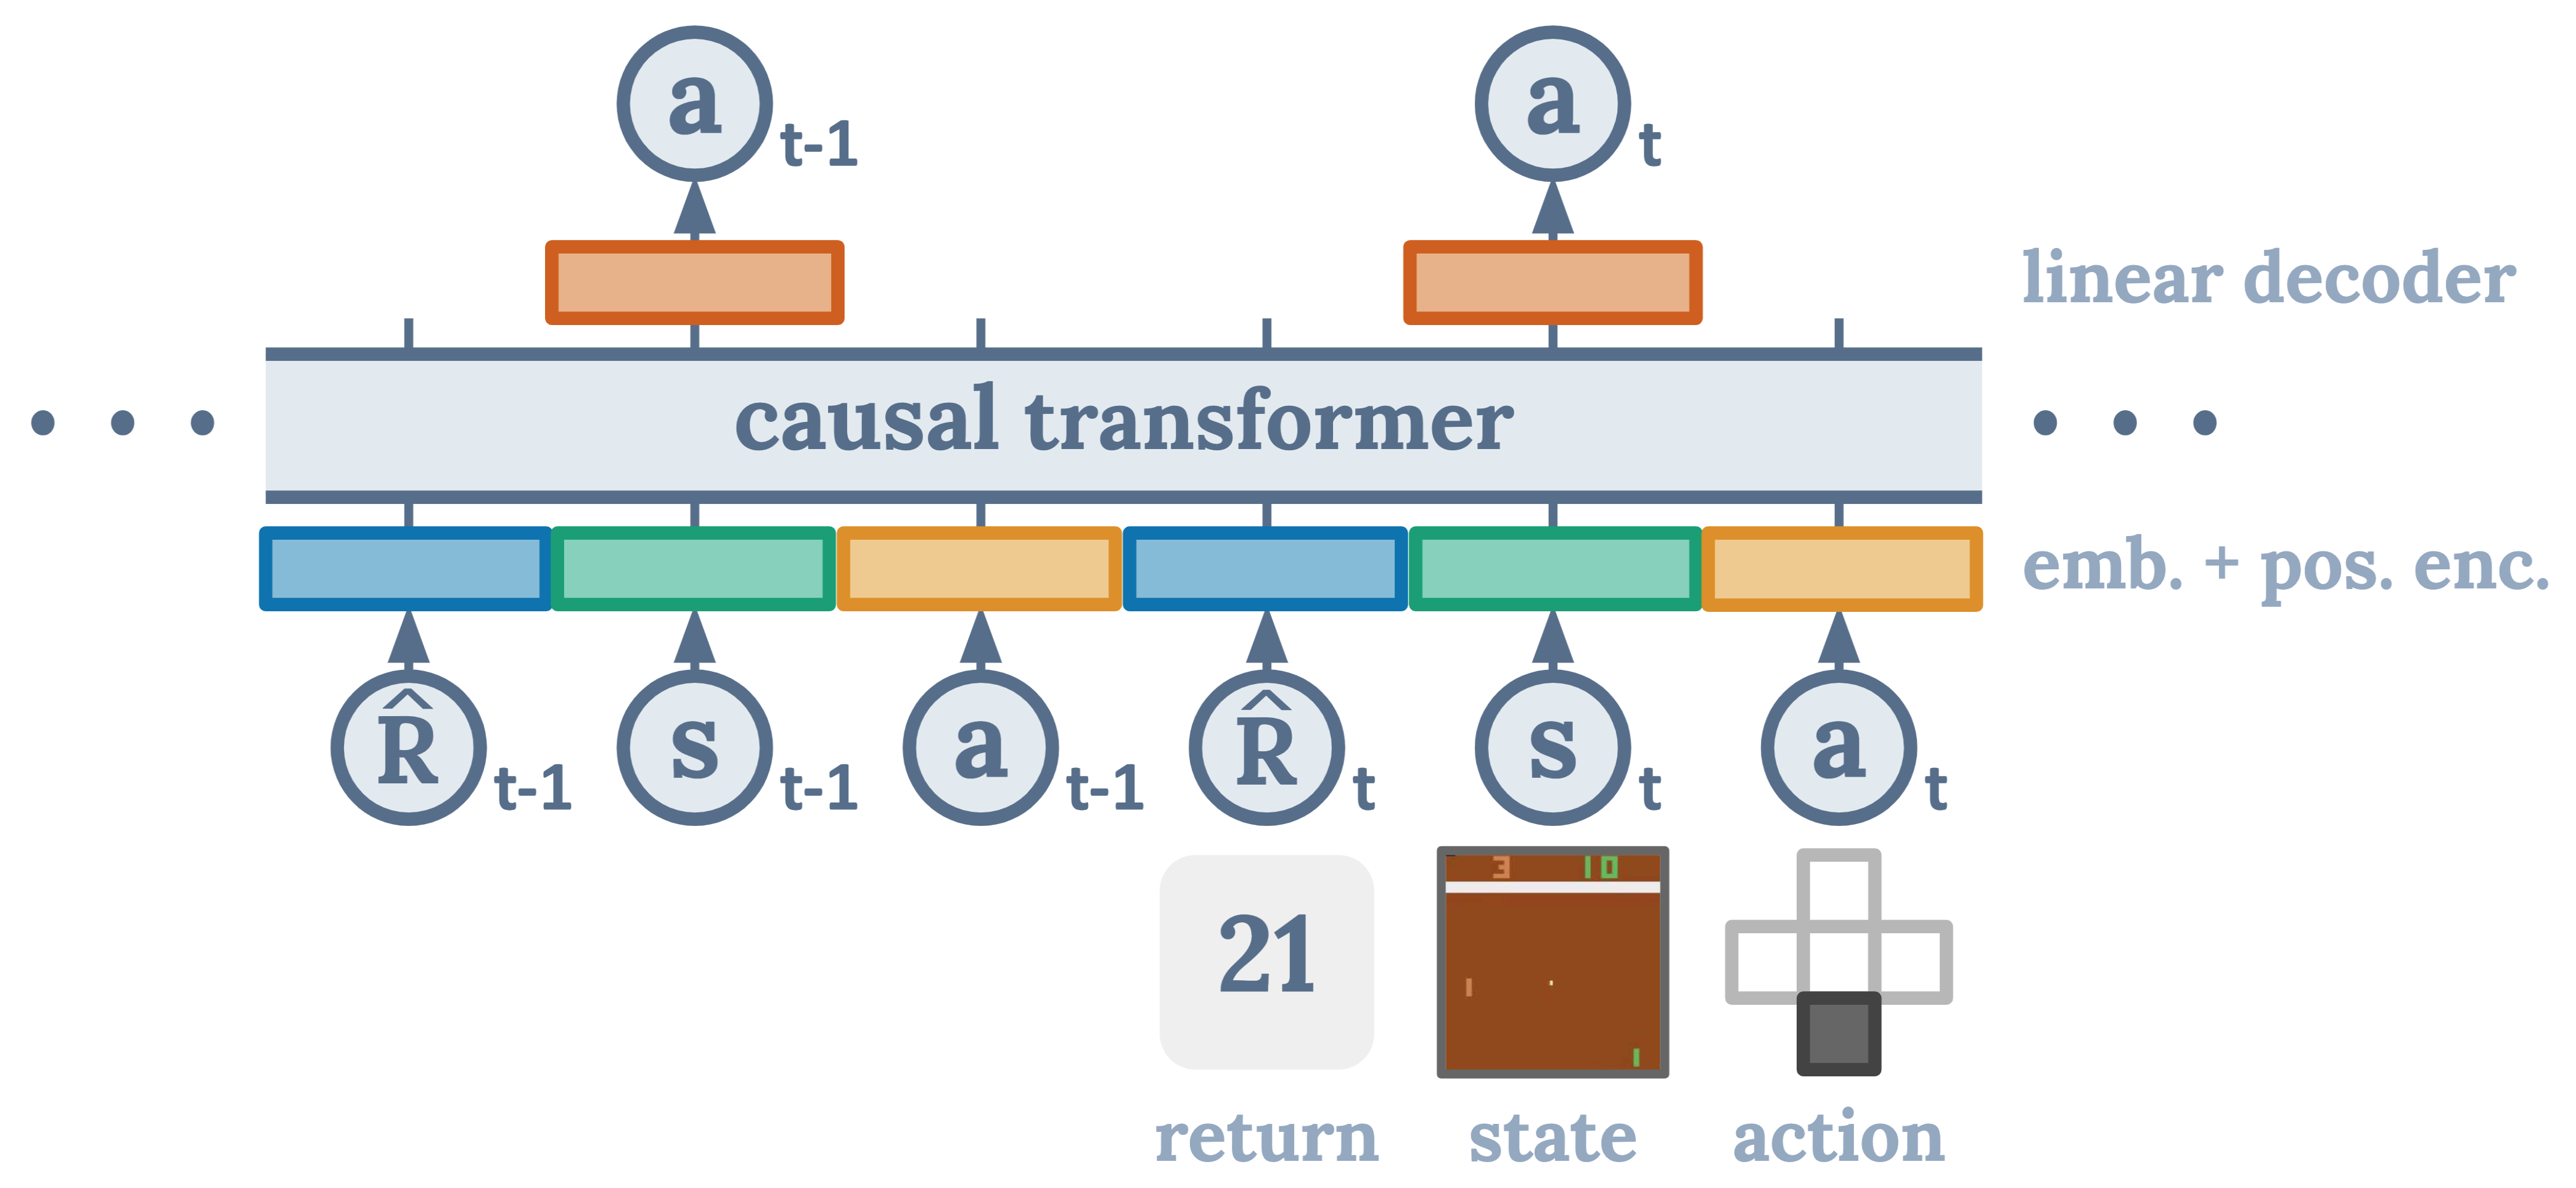
\includegraphics[width=0.8\textwidth]{figures/chap02/decision_transformer.png} 
\caption{Decision Transformer范式的工作框架\cite{chen2021decision}}
\label{fig:decision_trans_archi}
\end{figure}

Decision Transformer将一个将强化学习空间抽象为一个序列建模(Sequence Modeling)问题的框架,这有助于在模型选择时使用Transformer架构的模型,例如BERT\cite{koroteev2021bert}和GPT\cite{achiam2023gpt}类预训练大型语言模型,通过大规模并行的方式加快训练过程,并充分利用语言类生成模型的能力。

Decision Transformer相较于传统强化学习使用值函数(Q-Learning)或者策略梯度(Policy Gradient)的方式进行动作预测采用了截然不同的方式,它使用自回归的方式完成预测。通过将状态、动作和预期回报(Return-To-Go,RTG)编码成序列,Decision Transformer可以在不交互训练的情况下完成对最优动作的选择。



从图\ref{fig:decision_trans_archi}中可知,一个决策序列的预期回报(Return-To-Go,RTG)、状态(State)、动作(Action)按照时间先后通过特别的嵌入层(Embedding),并配置了对应的位置编码,通过一个Transformer类的模型通过一个线性映射层,输出了最新决策的动作。对应的状态转移、预期奖励和该动作又被作为下一个三元组继续进行动作决策,以自回归的方式做出新的决策。更具体的形式化描述可以表述为下列推导。

设定一个强化学习的序列状态 $s_t$、动作 $a_t$ 和奖励 $r_t$,其中$t$代表序列的决策时刻$1,2,...,T$,Decision Transformer利用该序列构建式\eqref{eq:three_deci}表示的三元组:
\begin{equation}
\begin{aligned}
    (R_1,s_1,a_1,R_2,s_2,a_2,...,R_T,s_T,a_T),
\end{aligned}
\label{eq:three_deci}
\end{equation} 

其中$R_t$代表Return-to-go,是Decision Transformer中特别的回报计算方式,统计从时间步$t$到终止时刻$T$的累计回报,用于告知模型优化的方向,如式\eqref{eq:rtg}所示:
\begin{equation}
\begin{aligned}
    R_t = r_t + \gamma r_{t+1} + \gamma^2 r_{t+2} + ... + \gamma ^{T-t}r_{T}.
\end{aligned}
\label{eq:rtg}
\end{equation} 

随后,$R_t$、动作 $a_t$ 和奖励 $r_t$分别通过各自的嵌入(Embedding)层完成到模型输入层的映射,并通过一个基于Transformer架构的模型,获得最终的输出动作决策。

Decision Transformer模型的预测是自回归的,给定过去的信息和目标回报,来预测当前的最优动作$\hat{a}_t$,可表示为式\eqref{eq:deci_at_goal}:
\begin{equation}
\begin{aligned}
    \hat{a}_t = f(R_t,s_t|R_{t-1},s_{t-1},a_{t-1},...).
\end{aligned}
\label{eq:deci_at_goal}
\end{equation} 


Decision Transformer训练时需要习得一个能够根据历史轨迹生成最优动作的策略,不通过实时与环境交互的方式,而是采用了有标签的监督学习方式进行训练,因此该方案更适配离线强化学习。其训练目标,即最小化的损失函数可以表示为式\eqref{eq:deci_trans_goal}:
\begin{equation}
\begin{aligned}
    L(\phi) = \mathbb{E}_{(R_t,s_t,a_t) \sim \mathcal{D}}\left[||a_t-\hat{a}_t||^2\right],
\end{aligned}
\label{eq:deci_trans_goal}
\end{equation}

其中$\mathcal{D}$是预先采集的离线强化学习决策轨迹构成的数据集,该数据集应该具有已经定义的奖励值作为选择评判标准;$a_t$ 表数据集中真实执行的动作,可能非最优解,亦作为部份轨迹使模型更全面习得决策结果的优缺点;$\hat{a}_t$则表示模型推测的结果。通过计算两个动作之间的L2范数平方误差,获得损失值,并最小化此损失值达成训练模型的目的。这种使用监督学习的方式能够避免贝尔曼方程计算的传播误差,直接建模了最优动作,同时利用了Transformer的长上下文感知特性,从而最大化了长期回报。


% !TeX root = ../thuthesis-example.tex

\chapter{场景时延敏感度可感知的传输速率控制}
\section{本章序言}
云游戏是实时通信(Real-time communication,RTC)技术进步的产物,它通过将游戏渲染任务卸载到服务器,并将其以实时视频格式流式传输给用户,从而减轻了用户设备的计算负担。因此,云游戏对RTC所支持的实时传输和游戏画面流畅度提出了更高的要求,使得速率控制策略在确保用户体验质量方面至关重要。

现有的速率控制方法,如延迟排队理论建模\cite{arun2018copa,raeis2021queue}、固定规则\cite{ray2022sqp,carlucci2016analysis}、强化学习\cite{abbasloo2020classic,jay2019deep}以及基于用户感知的方法\cite{peng2023pacc,huang2023optimizing},主要目标是实现超低延迟。然而,它们通常忽视了云游戏中的延迟敏感性问题\cite{claypool2006latency,claypool2010latency}。考虑到延迟敏感性可以在流媒体画质\cite{shang2021study} 和端到端延迟之间提供更好的平衡,这对于确保令人满意的用户体验至关重要。在云游戏中,流媒体画质通过比特率、流畅度和画面抖动等指标进行衡量。

本章研究通过进行大规模数据测量和用户平均意见得分(Mean Opinion Score,MOS)实验,观察到了不同游戏场景中延迟对用户满意度的影响存在差异。某些依赖于实时决策的游戏类型在延迟增加时表现出满意度的显著下降,而其他类型的游戏在有限的延迟范围内则相对不受影响。为了描述这种现象,本章节引入了“敏感性”这一概念,用于描述延迟对用户参与度的影响,其中更高的敏感性表示在延迟上升时满意度下降得更为显著。本章节在多个游戏场景下的实验结果揭示了游戏可以被分为潜在的三种敏感性类别:高敏感、中敏感和低敏感。

为了便于在算法设计中应用这些发现,本章节利用最小二乘估计将MOS得分映射到延迟感知敏感性曲线。这些曲线建立了各个游戏类型的可接受延迟范围与延迟影响程度之间的关系,为带宽受限下的延迟和画质权衡提供了灵活性。

在追求这种权衡下的最佳用户体验(Quality of Experience,QoE)时,强化学习(Reinforcement Learning,RL)成为一种有效的解决方案。尽管已有十年的强化学习视频传输优化研究\cite{dao2022contemporary},但将强化学习应用于云游戏流媒体仍存在空白,特别是考虑到游戏延迟敏感性分类的问题。现有的研究,如ReCoCo\cite{markudova2023recoco}和R3Net\cite{fang2019reinforcement},未能考虑云游戏中不同游戏应用的敏感性差异。

为此,本章节提出了Sense,一种针对云游戏服务定制的演员-评论家(Actor-Critic)速率控制算法。与先前主要关注最小化传输延迟的方法不同,Sense 利用延迟感知敏感性曲线,在延迟和视觉保真度之间的权衡过程中提供更大的灵活性。通过基于空间感知信息(Spatial Information,SI) 和时间感知信息(Temporal Information,TI)确定的游戏类别选择奖励函数,Sense 提升了整体用户体验质量。通过结合延迟感知敏感性曲线并评估视觉流畅度和比特率,Sense能够学习最优策略,在权衡过程中最大化QoE。Sense的核心概念如图\ref{fig:teaser}所示,利用云游戏中的延迟感知敏感性差异,重新设计了强化学习的状态空间和奖励函数。对于云游戏平台上的游戏场景,Sense通过TI和SI确定其敏感性分类(高、中、低),然后选择相应的延迟感知敏感性曲线。通过整合延迟感知敏感性曲线,并考虑发送比特率和视觉流畅度等因素,Sense在不同游戏场景下实现了延迟和流媒体画质之间的更精细平衡。

\begin{figure}[h]
    \centering
    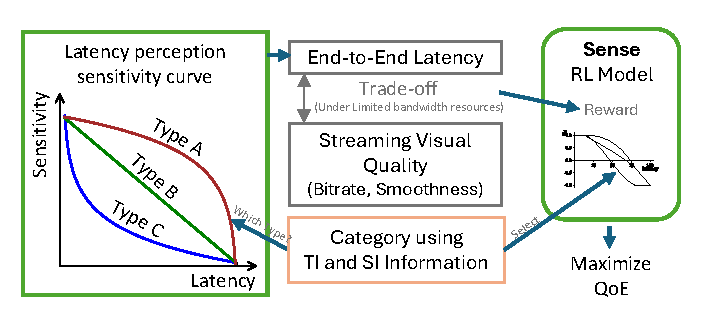
\includegraphics[width=0.78\textwidth]{figures/chap03/teaser.pdf}
    \caption{敏感度可感知的云游戏传输速率控制算法的设计框架}
    \label{fig:teaser}
\end{figure}

Sense的评估结果显示,它通过将延迟与各种场景类型对齐、减少画面抖动并准确分类场景敏感性,从而提高了QoE分数和场景分类准确性。

总结来说,本章节的贡献包括:
\begin{itemize}

\item 进行用户MOS实验,识别不同场景中的三种敏感性类型,并使用最小二乘估计拟合高、中、低敏感性的延迟感知敏感性曲线。
  
\item 提出Sense,一种专门为云游戏服务定制的Actor-Critic架构的强化学习速率控制算法。Sense在不同游戏场景中实现了延迟和画质之间的更好平衡,QoE提高了16.7\%。

\item 使用视频流信息(即时间感知信息TI和空间感知信息SI)对游戏场景的敏感性进行分类,准确率达到89.4\%,从而减少了对每个游戏的用户敏感性打分实验依赖。
\end{itemize}


\section{主客观测量实验和动机}
\subsection{数据测量与结果分析}\label{sec-measurement-study}
云游戏平台上有许多不同的场景和游戏。ClayPool等人的研究\cite{claypool2010latency}表明,游戏有不同的“阶段”,如“启动”、“同步”和“过渡”。这些阶段表现出显著的比特率差异,表明场景动态和延迟要求的变化。此外,不同的游戏类型,如第一人称射击游戏(First Person Shooting,FPS)、多人在线战术竞技场(Multiplayer Online Battle Arena,MOBA)、体育游戏(Sports Game)和集换式卡牌游戏(Collectible Card Game,CCG),在游戏过程中对延迟的敏感性各不相同。该研究还为不同的游戏提供了截止时间阈值。例如,射击游戏重度依赖于实时反应,而集换式卡牌游戏场景则优先考虑沉浸式体验,注重流畅的游戏过程和高质量的视觉效果。这些游戏的常见场景画面如图\ref{fig-game-sample}所示。
\begin{figure}[ht]
\centering
\begin{subfigure}[t]{0.4\linewidth}
  \centering
  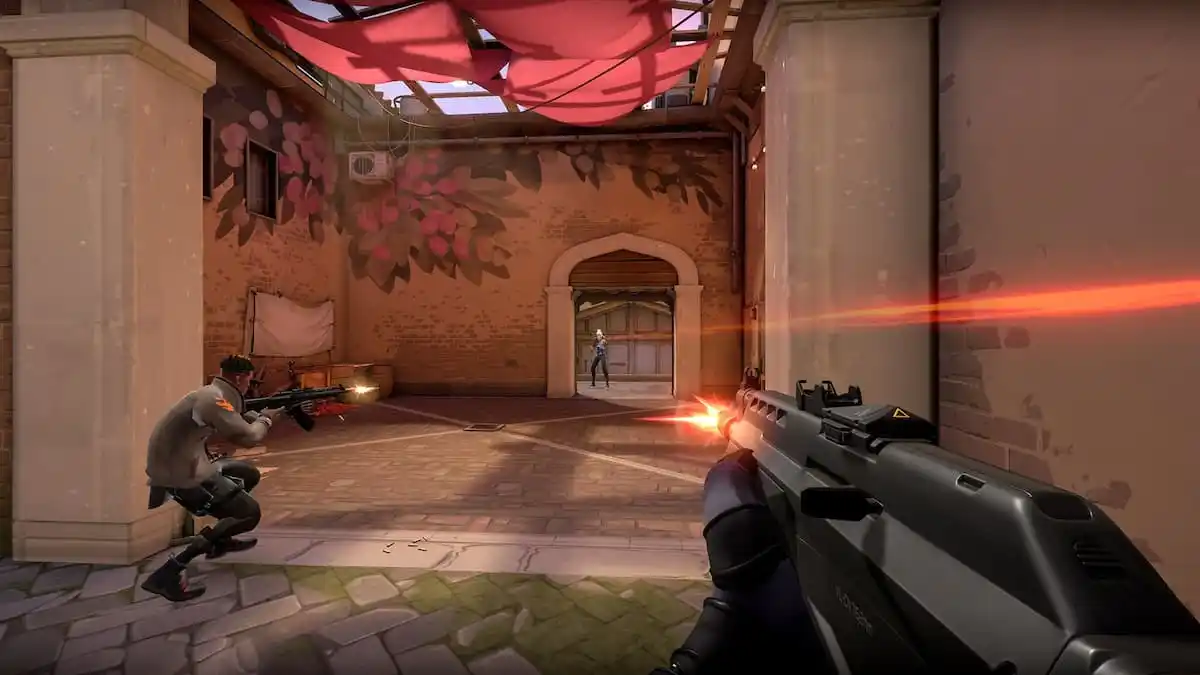
\includegraphics[width=\linewidth]{figures/chap03/game_example/fps_game.png}
  \caption{FPS 游戏}
  \label{fig-fps-game}
\end{subfigure}%
\begin{subfigure}[t]{0.4\linewidth}
  \centering
  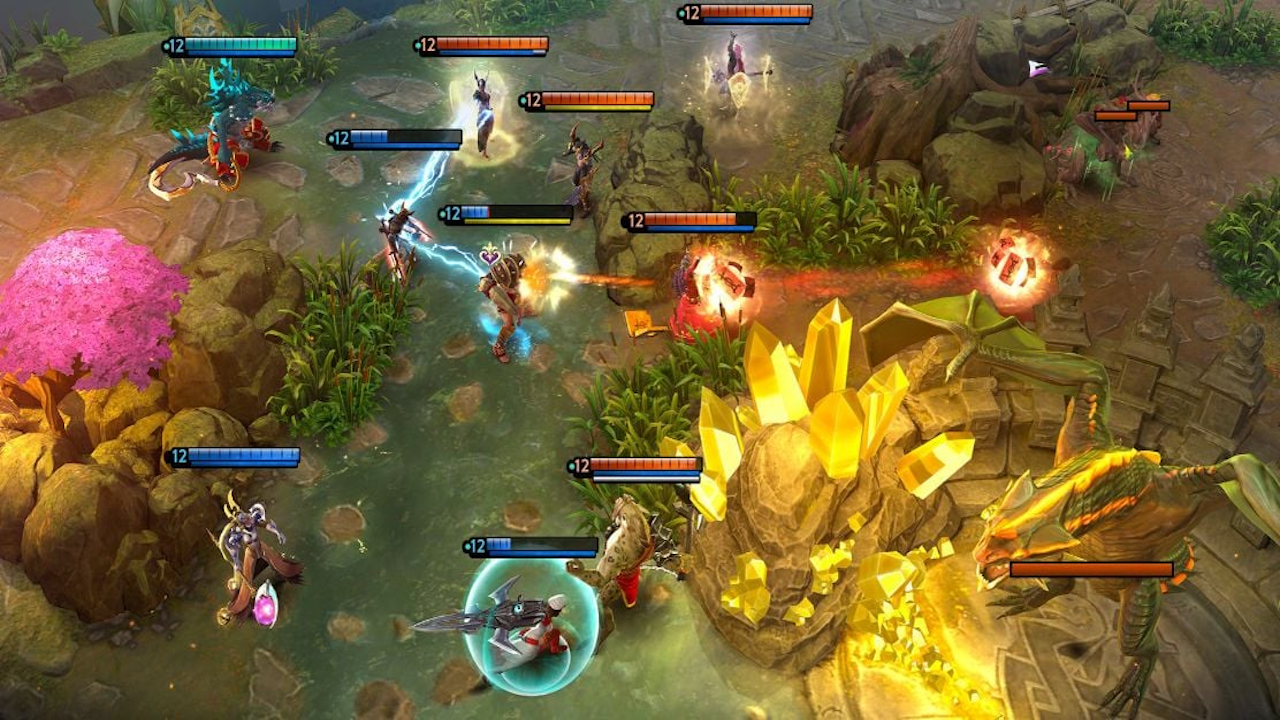
\includegraphics[width=\linewidth]{figures/chap03/game_example/moba_game.png}
  \caption{MOBA 游戏}
  \label{fig-moba-game}
\end{subfigure}

\begin{subfigure}[t]{0.4\linewidth}
  \centering
  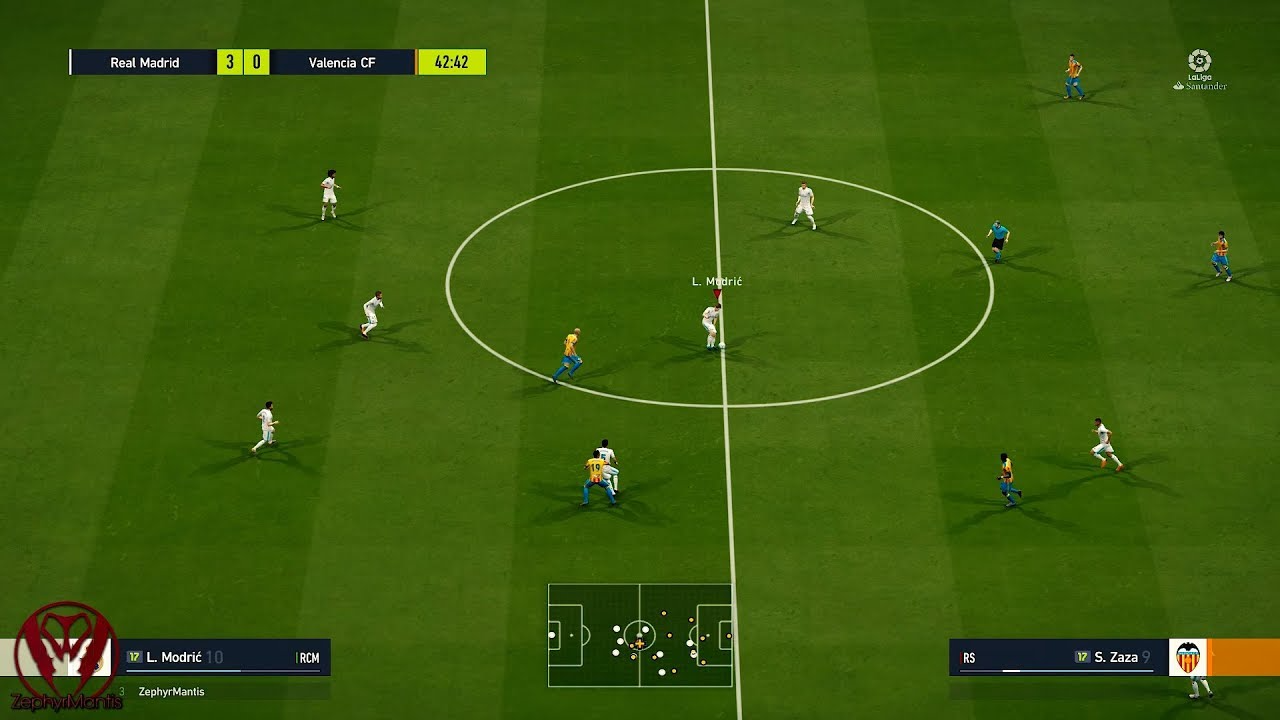
\includegraphics[width=\linewidth]{figures/chap03/game_example/sport_game.png}
  \caption{体育游戏}
  \label{fig-sport-game}
\end{subfigure}%
\begin{subfigure}[t]{0.4\linewidth}
  \centering
  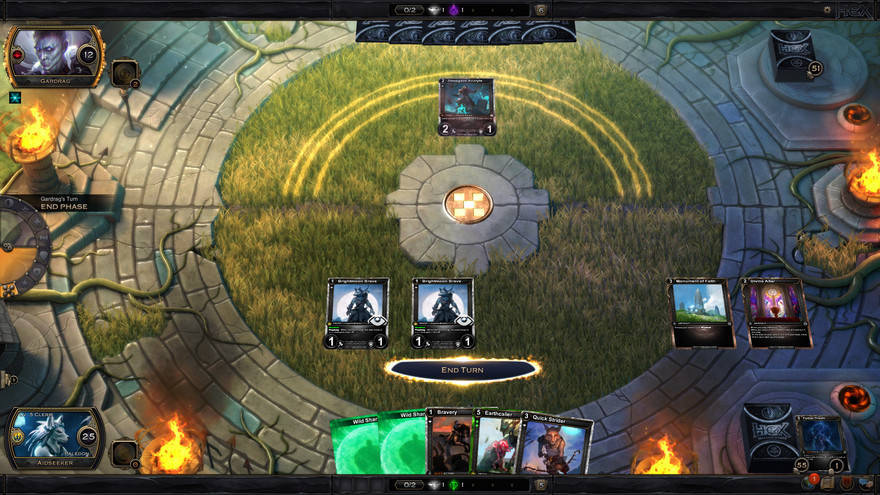
\includegraphics[width=\linewidth]{figures/chap03/game_example/chess_game.png}
  \caption{集换式卡牌游戏}
  \label{fig-chess-game}
\end{subfigure}

\caption{不同类型游戏的常见场景示例}
\label{fig-game-sample}
\end{figure}


\subsubsection{系统运行架构和时间延迟测量方式}
云游戏将渲染和其他计算密集型处理过程转移到强大的云服务器上,并将渲染后的视频流传输到用户设备,类似于视频流服务的工作方式。此外,云游戏还包括实时的用户交互。因此,衡量用户在云游戏中感知到的延迟的一个关键方式是使用“操作到画面”(Motion-to-Photon,MTP)延迟。延迟的主要来源如图\ref{fig_system_architecture}所示。

\begin{figure} [ht]
\centering
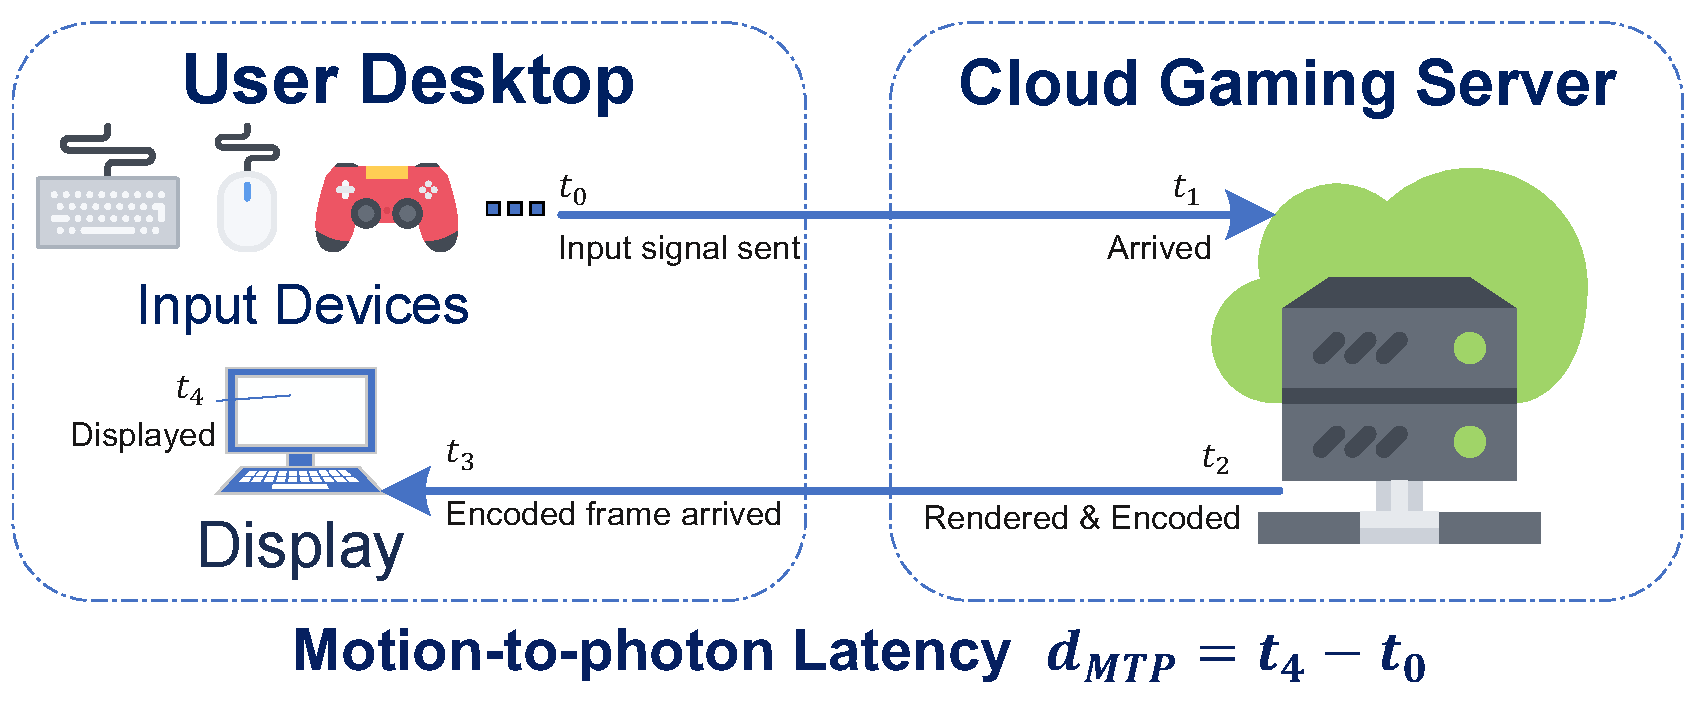
\includegraphics[width=0.7\textwidth]{figures/chap03/system_architecture.pdf} 
\caption{云游戏实时通信系统的架构及时刻}
\label{fig_system_architecture}
\end{figure}

一旦用户在时间 $t_0$ 触发操作,请求会由于网络延迟在时间 $t_1$ 到达服务器。服务器完成游戏画面的渲染并使用低延迟编码器进行编码,编码在时间 $t_2$ 完成。然后,数据包到达用户设备并在时间 $t_3$ 解码。最后,视频流完全解码并显示在用户屏幕上,时间为 $t_4$。MTP 延迟考虑了从 $t_0$ 到 $t_4$ 的整个处理延迟,并定义为 $d_{MTP} = t_4 - t_0$,即用户执行操作与该操作显示在屏幕上的时间差。这种方法提供了用户感知的延迟的更准确测量,从而更精确地评估云游戏中的QoE。

\subsubsection{大规模数据测量}
为了研究不同应用在云游戏实时通信平台上对延迟效应的QoE敏感性,本工作在一个商业平台上进行了为期一年的大规模测量研究。数据集包含超过350万条验证记录,最细粒度为单个连接的建立到终止的过程。为了减少真实生产环境中可能出现的混杂因素的影响,本工作采用了多个标准来筛选大量在线数据,包括由用户发起但没有后续活动的连接,以及持续时间过短的连接。被测量的游戏及每款游戏使用的数据集如表\ref{table_flow_count}所示。数据有两种不同粒度类型:流粒度持续时间是指从用户发起连接请求开始,直到用户关闭连接为止,形成一组统计数据为一次统计,作为单条数据进行使用的数据;而帧粒度持续时间则是指单个流中每一帧画面显示为一次统计,一个流形成一张表格。后者的粒度比前者更细,可以获得更多细节统计信息,收集用于进一步探索,两者共同使用形成测量结果。

\begin{table}[ht]
\centering
\caption{用于统计游戏的流属性统计}
\begin{tabular}{@{}ccccc@{}}
\toprule
\textbf{游戏}        & \textbf{流粒度持续时间(小时)} & \textbf{帧粒度持续时间(小时)} \\ \midrule
2D-RPG I             & 3707.74                  & 910.23                    \\
2D-RPG III           & 2558.73                  & 460.17                    \\
3D-RPG I             & 889.68                   & 49.83                     \\
动作游戏 I           & 1194.60                  & 102.73                    \\
A-RPG I              & 529.15                   & 87.37                     \\
休闲游戏 I           & 70.47                    & 3.29                      \\
CCG I                & 200.42                   & 12.80                     \\
FPS I                & 1360.89                  & 277.21                    \\
FPS II               & 151.32                   & 79.51                     \\
FPS III              & 570.81                   & 62.75                     \\
FPS IV               & 281.95                   & 20.71                     \\
MMORPG I             & 638.79                   & 82.72                     \\
MOBA I               & 685.65                   & 378.66                    \\
MOBA II              & 247.16                   & 98.07                     \\
运动游戏 I           & 1068.06                  & 249.90                    \\
运动游戏 II          & 155.76                   & 35.31                     \\
运动游戏 III         & 1376.29                  & 0.13                      \\
TPS I                & 331.30                   & 25.43                     \\ \bottomrule
\end{tabular}
\label{table_flow_count}
\end{table}



从大规模测量中获得的原始数据,由于记录中存在异常使用数据,往往偏离理想数据。为了确保数据测量的准确性,需要应用某些规则,尽可能排除由于用户或设备链路问题导致的异常数据。可能的异常数据情况包括:
\begin{itemize} 
\item \textbf{用户提前退出:}该情况指的是用户与服务器建立连接后,但未实际进行游戏便退出。此类连接通常持续时间较短,不超过 2 分钟。 

\item \textbf{僵尸流量:}该情况指的是客户端与服务器的连接异常断开,但流量未停止并继续计数,导致数据不正确。这样可能导致流量被计量几个小时甚至超过一天,超过了正常可接受的长时间使用时长。 

\item \textbf{频繁切换网络:}为了排除用户网络连接不稳定的情况,测量中选择常见的网络类型(2.4GHz 和 5GHz Wi-Fi、以太网或蜂窝数据)。在单次连接中,频繁切换网络连接的情况将不被纳入统计。 

\item \textbf{极低的实际编码比特率:}实际编码比特率低于设置比特率的十分之一,通常是由于长时间静态或极小的画面,导致需要传输的残余信息非常少,从而导致极低的比特率。这表明尽管用户已连接,但并未进行任何操作。 

\item \textbf{低交互频率}:用户客户端接收到的输入频率极低,如键盘、鼠标或游戏手柄的输入频率。此类情况也表明用户已建立连接,但未进行任何游戏活动。 

\item \textbf{异常的客户端处理时间:}通常,在性能稳定的机器上接收和解码视频不应超过某个时间限制。处理时间波动较大或连接时间过长的情况也应排除。在处理延迟过高的情况下,用户无法正常游戏,而连接时间过长则表明客户端存在异常行为,因此需要排除。 

\end{itemize}

游戏选择包括平台上的九款主流热门游戏:第一人称射击(First Person Shooting,FPS)游戏I、II、III,2D角色扮演(RPG)游戏I、II,体育游戏I,集换式卡牌游戏(Collectible Card Game,CCG)I,以及多人在线战术竞技(Multiplayer Online Battle Arena,MOBA)游戏I、II。这些热门游戏具有大量数据流量,并涵盖了传统意义上不同类型和类别的游戏,代表了不同游戏应用在云游戏实时通信系统上的差异。

不同类型游戏对MTP延迟的敏感性如图\ref{fig-real-measurement-results-High-Delay-Sensitivity-Games}、\ref{fig-real-measurement-Medium-Delay-Sensitivity-Games} 和 \ref{fig-real-measurement-results-Low-Delay-Sensitivity-Games} 所示。为了反映用户参与度,测量选择使用时间作为主要指标,研究MTP延迟与用户参与度之间的关系。由于游戏时长可能受关卡设计或回合时长等因素的影响,测量对游戏时长进行了归一化处理。归一化过程包括计算每个游戏的平均使用时间,并与单个游戏回合的典型时长进行验证。如果平均使用时间明显短于单个游戏回合所需的最小时长,则认为数据存在混杂因素,并进一步进行筛选。确认正确的平均使用时间后,所有测得的使用时间将除以上述平均值,得到相对于平均游戏使用时间的百分比。通过这种方式,每个游戏的标准使用时间在y轴上归一化为1.0x,从而更容易观察相对时长。游戏被分为三类:高敏感度、中敏感度和低敏感度游戏。随着MTP延迟的增加,图\ref{fig-real-measurement-results-High-Delay-Sensitivity-Games} 中的三类游戏的游玩时长表现出初期的指数级下降,而图\ref{fig-real-measurement-Medium-Delay-Sensitivity-Games} 中则呈现更接近线性的下降,不同游戏的时长下降至0.6 - 0.8x。相比之下,图\ref{fig-real-measurement-results-Low-Delay-Sensitivity-Games} 中的游戏在某一延迟阈值(大约35ms)之前,游玩时长没有显著下降,超过该阈值后,游玩时长降至0.8x - 0.95x。
\begin{figure}[htbp]
\centering
\begin{subfigure}[t]{0.4\linewidth}
  \centering
  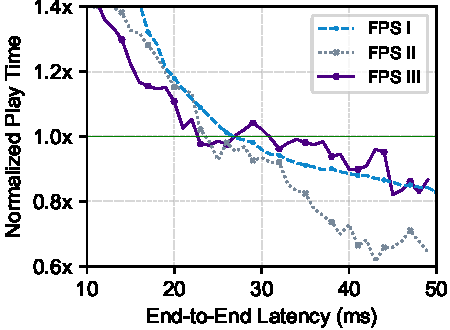
\includegraphics[width=\linewidth]{figures/chap03/measurement_data/delay-sensitive.pdf}
  \caption{高敏感度游戏}
  \label{fig-real-measurement-results-High-Delay-Sensitivity-Games}
\end{subfigure}%
\begin{subfigure}[t]{0.4\linewidth}
  \centering
  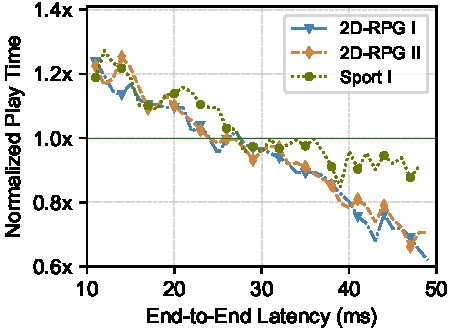
\includegraphics[width=\linewidth]{figures/chap03/measurement_data/delay-linear-sensitive.pdf}
  \caption{中敏感度游戏}
  \label{fig-real-measurement-Medium-Delay-Sensitivity-Games}
\end{subfigure}

\begin{subfigure}[t]{0.4\linewidth}
  \centering
  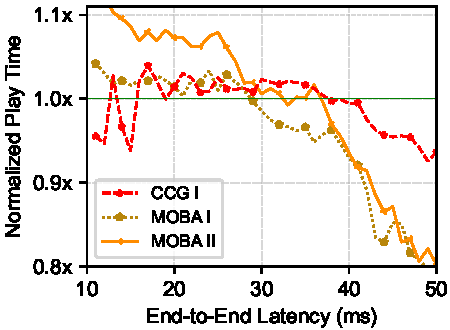
\includegraphics[width=\linewidth]{figures/chap03/measurement_data/delay-not-sensitive.pdf}
  \caption{低敏感度游戏}
  \label{fig-real-measurement-results-Low-Delay-Sensitivity-Games}
\end{subfigure}%
\begin{subfigure}[t]{0.4\linewidth}
  \centering
  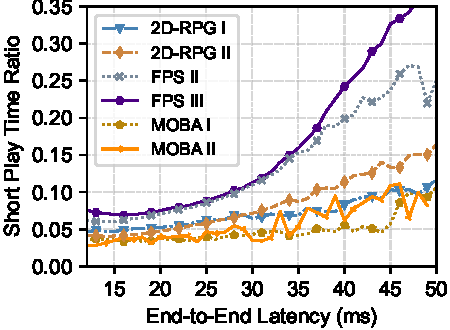
\includegraphics[width=\linewidth]{figures/chap03/measurement_data/early_quit_ratio.pdf}
  \caption{短时游玩比例}
  \label{fig-real-measurement-results-Short-Play-Time-of Games}
\end{subfigure}

\caption{不同敏感度的游戏在平均时延下的使用时长}
\label{fig:measurement-result}
\end{figure}


由于大多数游戏要求用户参与实时游戏,且无法像观看视频那样随意退出,因此使用像 \cite{chengrebuffering} 中的退出率已经不再可靠。测量中定义了短时游戏时长的概念,并将每个游戏的平均游戏时长的50\%作为短时游戏时长的阈值。在图\ref{fig-real-measurement-results-Short-Play-Time-of Games} 中,测量观察了在不同平均延迟条件下,用户进行短时游戏时长的概率。可以看出,高延迟敏感游戏的退出率随着延迟的增加显著加快,而中低延迟敏感游戏的退出率增长大约在5\%到10\%之间,低延迟敏感游戏的影响略小。


有趣的是,当直接绘制原始数据时,可以从测量结果中观察到因素之间呈现出非单调关系,这与 \cite{balachandran2013developing} 中的测量结果非常相似,在特定的延迟值处存在多个峰值。在数据过滤后,这一趋势变得不那么显著,但仍然存在,确认了这一非单调关系的出现是由于频繁的延迟波动导致了平均延迟的下降和QoE的下降。

\subsection{用户MOS实验}\label{sec-mos}

测量实验说明了游戏敏感度的区分可分为高、中、低三个敏感度。为了进一步研究不同场景下延迟差异和用户满意度要求,研究开展了在不同场景下的平均意见得分(MOS)评分测试,以评估用户在特定延迟条件下的满意度水平。实验包括20名参与者,他们的画像如表\ref{tab:userinfo}所示。

\begin{table}[ht]

\caption{参与者的基本信息}
\renewcommand\arraystretch{1.25}

\begin{center}

\begin{tabular}{@{}ccccc@{}}
\toprule
\multicolumn{2}{c}{游戏类型}                       & FPS & \begin{tabular}[c]{@{}c@{}}MOBA 和 CCG\end{tabular} & \begin{tabular}[c]{@{}c@{}}RPG 和 体育\end{tabular} \\ \midrule
\multicolumn{2}{c}{参与者人数}                   & 5   & 9                                                  & 6                                                   \\ \hline
\multirow{3}{*}{年龄}                & 18-22岁    & 2   & 4                                                  & 2                                                   \\
                                 & 23-26岁    & 2   & 3                                                  & 2                                                   \\
                                 & 27-30岁    & 1   & 2                                                  & 2                                                   \\ \hline
\multirow{3}{*}{游戏经验}          & 初学者     & 1   & 1                                                  & 1                                                   \\
                                 & 中级       & 2   & 4                                                  & 3                                                   \\
                                 & 高级       & 2   & 4                                                  & 2                                                   \\ \bottomrule
\end{tabular}
\end{center}
\label{tab:userinfo}
\end{table}


共获得220条有效记录,且没有引发伦理问题。为了模拟网络连接中的端到端延迟,实验使用了 NetEm 和 TC(流量控制)在服务器和用户设备之间建立了专用网络连接。在预定义的时间间隔内,用户提供了5分制MOS评分,反映他们的游戏体验。MOS评分为3被设定为用户满意或不满意的临界值。具体的MOS评分含义包括在了表\ref{tab:mos_rate}中。

\begin{table}[ht]
    \caption{用户MOS评分值的含义}
    \renewcommand\arraystretch{1.25}
    \centering
    \begin{tabular}{@{}cc@{}}
\toprule
评分 & 含义                                                           \\ \midrule
5     & 高清晰度和平滑画面,非常即时的响应。                          \\
4     & 相当清晰和平滑的画面,较为即时的响应。                        \\
3     & 平均视觉质量,满足最低响应要求。                              \\
2     & 画面有些卡顿和延迟,响应不够即时。                            \\
1     & 无法接受的视觉质量,响应缓慢影响游戏体验。                   \\ \bottomrule
\end{tabular}
    \label{tab:mos_rate}
\end{table}


调查结果的平均值如图\ref{fig-average-user-mos-rating}所示,将游戏分为高、中、低三种敏感性类别。结果显示,不同游戏类型对增加的端到端延迟的敏感性各不相同。这一发现表明,可以将原本用于减少延迟的资源重新分配到在带宽受限的情况下提升视觉质量。通过在延迟和视觉质量之间进行平衡,云游戏平台可以优化资源分配,改善整体游戏体验,特别是在延迟不那么关键的场景中。
\begin{figure}[ht]
\centering
\begin{subfigure}[t]{0.49\linewidth}
  \centering
  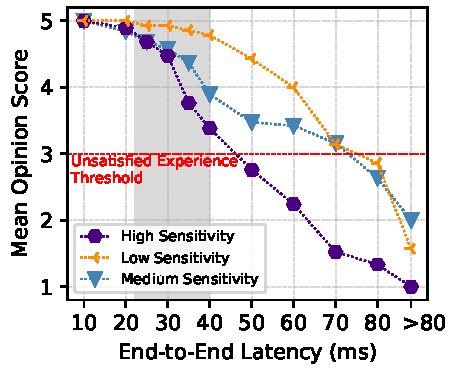
\includegraphics[width=\linewidth]{figures/chap03/latency_curve/user_perception.pdf}
  \caption{用户平均MOS评分}
  \label{fig-average-user-mos-rating}
\end{subfigure}%
\begin{subfigure}[t]{0.49\linewidth}
  \centering
  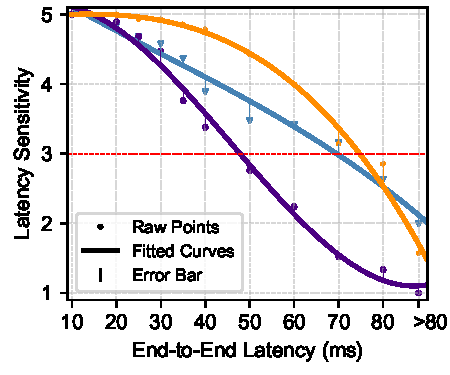
\includegraphics[width=\linewidth]{figures/chap03/latency_curve/fitted_curve.pdf}
  \caption{拟合曲线}
  \label{fig-fitted-curves}
\end{subfigure}

\caption{用户MOS评分实验结果和数值拟合结果}
\label{fig-latency-curve}
\end{figure}



\subsection{测量结果使用方案和设计挑战}
利用云游戏平台中不同应用的延迟敏感性为流媒体传输中的发送速率适应性调整提供了机会,从而在延迟和视觉质量之间实现更好的平衡,最终提升用户体验质量。然而,目前云游戏平台如何将测量结果揭示的敏感性特征融入其速率控制算法中仍存在空缺。弥补这一空缺需要克服若干挑战。

\textbf{挑战一:敏感性的量化。} 虽然实验结果提供了关于不同游戏场景对延迟敏感性的定性见解,但缺乏一种系统化、可量化的度量方法,使得延迟对用户体验的具体影响难以直接衡量。开发一个感知函数来评估敏感性水平对于实现这一目标至关重要。该函数应该能够以形式化的数学表达准确反映延迟对用户体验的实际影响,进而将其映射到算法的设计中。

\textbf{挑战二:速率控制算法的设计。} 在不同的游戏场景下,延迟与视觉质量的平衡关系存在较大差异,因此所设计的速率控制算法必须能够自适应地适应不同延迟敏感性需求,而通过自适应学习在波动的网络条件下实现最大化用户体验质量的最终目标是一项复杂的决策任务。

\textbf{挑战三:确定场景延迟敏感性。} 不同的应用场景对延迟的敏感程度各不相同,如何基于客观指标准确地确定当前场景的敏感性分类对于最终的框架设计和实施至关重要。

\section{时延敏感性曲线拟合分析}\label{sec-latency-curve} 
通过进行MOS评分实验,本实验获得了在不同延迟值下,用户的平均评分 $r_j$ 和对应的延迟值 $d_j$,如式\eqref{eq:djrj}所示: 
\begin{equation}
\begin{aligned}
    (d_j, r_j),  j= 1, 2, ..., m.
\end{aligned}
\label{eq:djrj}
\end{equation}

本章节利用最小二乘估计(Least Square Estimate,LSE)对特定延迟下的平均用户评分进行回归分析,从而得到拟合的延迟感知敏感度曲线。
令 $f(d)$ 是一个在 $m+1$ 个节点上定义的离散函数,其中 $a = d_0 < d_1 < \dots < d_m = b$,即 $f(d)$ 由式\eqref{eq:point}表示的点组成:
\begin{equation}
\begin{aligned}
    (d_j, f(d_j) = r_j),  j= 1, 2, ..., m.
\end{aligned}
\label{eq:point}
\end{equation}
$d_j$ 表示系统的端到端延迟,$r_j = f(d_j)$ 表示用户的 MOS 评分。同时,有一组在区间 $[a,b]$ 上定义的线性无关函数 $\varphi_0(d), \varphi_1(d), ..., \varphi_n(d)$,它们构成了 $\Phi = span\{\varphi_0, \varphi_1, ..., \varphi_n\}$。

为了拟合 $f(d)$,使用了LSE来得到最优化的函数 $s^* \in \Phi$,使得满足式\eqref{eq:satsify}的条件:
\begin{equation}
\begin{aligned}
    \sum^{m}_{j=0}[f(d_j)-s^*(d_j)]^2 = \min_{s \in \Phi} \sum^{m}_{j=0}[f(d_j)-s(d_j)]^2,
\end{aligned}
\label{eq:satsify}
\end{equation}
由于 $s \in \Phi$,可以表示 $s(d) = \sum^{n}_{i=0}a_i\varphi_i(d)$。这个问题现在转化为寻找式\eqref{eq:minpro}所示函数的最小值:
\begin{equation}
\begin{aligned}
    F(a_0, a_1, ..., a_n) = \sum^{m}_{j=0}\left[f(d_j)-\sum^{n}_{i=0}a_i\varphi_i(d_j)\right],
\end{aligned}
\label{eq:minpro}
\end{equation}
而$F(a_0, a_1, ..., a_n)$ 达到最小值的必要条件如式\eqref{eq:conddi}所示。
\begin{equation}
\begin{aligned}
    \frac{\partial F}{\partial a_k} = -2\sum^{m}_{j=0}\left[f(d_j)-\sum^{n}_{i=0}a_i\varphi_i(d_j)\right]\varphi_k(d_j)= 0, k = 0, 1, ..., n.
\end{aligned}
\label{eq:conddi}
\end{equation}


现定义式\eqref{eq:condi}:
\begin{equation}
\begin{aligned}
(\varphi_i,\varphi_k) =& \sum^{m}_{j=0}\varphi_i(d_j)\varphi_k(d_j),\\ 
(f,\varphi_k) =& \sum^{m}_{j=0}f(d_j)\varphi_k(d_j),
\end{aligned}
\label{eq:condi}
\end{equation}
可以将式\eqref{eq:condi}简化为式\eqref{eq:simple}:
\begin{equation}
\begin{aligned}
\sum^{n}_{i=0}(\varphi_i,\varphi_k)a_i = (f,\varphi_k), k = 0, 1, ..., n.
\end{aligned}
\label{eq:simple}
\end{equation}
这是一个非齐次线性方程组,当系数矩阵非奇异时,可以解出式\eqref{eq:mat}:
\begin{equation}
\begin{aligned}
\begin{bmatrix}  
  (\varphi_0,\varphi_0) & (\varphi_0,\varphi_1) & \cdots & (\varphi_0,\varphi_n) \\  
  (\varphi_1,\varphi_0) & (\varphi_1,\varphi_1) & \cdots & (\varphi_1,\varphi_n) \\  
  \vdots & \vdots & \ddots & \vdots \\  
  (\varphi_n,\varphi_0) & (\varphi_n,\varphi_1) & \cdots & (\varphi_n,\varphi_n)  
\end{bmatrix} \begin{bmatrix}  
   a_0 \\  
  a_1 \\  
  \vdots \\  
  a_n  
\end{bmatrix}  = \begin{bmatrix}  
   (f,\varphi_0) \\  
  (f,\varphi_1) \\  
  \vdots \\  
  (f,\varphi_n)
\end{bmatrix}.\end{aligned}
\label{eq:mat}
\end{equation}

对于用户评分数据,拟合过程选择使用最小二乘法拟合三次多项式、四次多项式、指数函数和对数函数。三次多项式的拟合结果获得了最小的误差,分别对应于三条灵敏度曲线,如图\ref{fig-fitted-curves} 所示。该曲线可以用式\eqref{eq:expr}表示:
\begin{equation}
\begin{aligned}
r = a_3 \cdot d^{3} + a_2 \cdot d^{2} + a_1 \cdot d + a_0,
\end{aligned}
\label{eq:expr}
\end{equation}
其中 $a_j$ 如表\ref{tab:a3a2a1a0}所示。


\begin{table}[ht]
\caption{使用三次多项式拟合用户评分的多项式系数}
\renewcommand\arraystretch{1.25}
\centering
% \resizebox{0.6\columnwidth}{!}{%
\begin{tabular}{@{}ccccc@{}}
\toprule
\textbf{}                              & \textbf{$a_3$}          & \textbf{$a_2$}          & \textbf{$a_1$}         & \textbf{$a_0$} \\ \midrule
\multicolumn{1}{c|}{\textbf{高敏感性}}  & $1.498 \times 10^{-5}$   & $-2.075 \times 10^{-3}$   & $2.130 \times 10^{-2}$  & $5.088$        \\

\multicolumn{1}{c|}{\textbf{中敏感性}} & $- 2.060 \times 10^{-6}$ & $1.863 \times 10^{-4}$   & $-3.862 \times 10^{-2}$ & $5.480$        \\
\multicolumn{1}{c|}{\textbf{低敏感性}}  & $- 4.580 \times 10^{-6}$ & $- 6.599 \times 10^{-5}$ & $4.117 \times 10^{-3}$  & $4.973$        \\ \bottomrule
\end{tabular}
% }
\label{tab:a3a2a1a0}
\end{table}


\section{场景需求可感知传输速率控制算法设计}
本章节中阐述了一个基于 Actor-Critic 架构的强化学习速率控制算法的设计,该算法利用延迟感知敏感度曲线为云游戏平台上的不同场景提供不同的速率调整策略。为了应对场景的敏感度分类问题,本章节利用了视频的空间感知信息(Spatial Information,SI) 和时间感知信息(Temporal Information,TI) 提供的信息来解决这一问题。

\subsection{感知强化学习空间设计}\label{sec:rl-design}
将强化学习的概念应用于速率控制问题,可以将网络视为观察环境,代理则根据当前的网络状态做出发送速率的决策。设定了一个固定的时间间隔 $\Delta t$ 为 200 毫秒,用于观察和决策。实验重新设计了强化学习的状态空间和动作空间。奖励函数由延迟、视频流畅度和与网络相关的指标组成,这些指标能够反映视觉质量和用户体验的质量。

\subsubsection{状态空间}
状态空间由网络状态的历史统计值构成。网络在固定时间间隔 $\Delta t = 200$ 毫秒内收集以下状态信息:(i)平均接收速率 $RR$,计算为每毫秒内所有接收数据包负载字节的总和的平均值;(ii)平均端到端延迟 $D$;(iii)数据包丢失率 $L$;(iv)帧间到达时间序列 $J$;(v)上一步采取的动作 $a$,即 $\boldsymbol{s_t} = (RR_t, D_t, L_t, J_t, a_t)$。选择过去 5 个值作为状态向量的组成部分,这对应于过去一秒钟的记录:$\mathcal{S}t = (\boldsymbol{s_t}, \boldsymbol{s{t-1}}, ..., \boldsymbol{s_{t-4}})$。


\subsubsection{动作空间}
动作空间设置为每个时间周期内发送速率的决策值。决策值可以选择在 $[3, 50]$ Mbps 范围内,以确定传输速率。为了在训练过程中保持性能稳定,实验设计使用对数函数将发送速率 $R_s$ 的范围归一化到 $[0, 1]$,如式\eqref{eq:logsend}所示:

\begin{equation}
\begin{aligned}
    R_{slog} = \frac{\log(R_s)-\log(R_{min})}{\log(R_{max})-\log(R_{min})}.
\end{aligned}
\label{eq:logsend}
\end{equation} 

\subsubsection{奖励函数}
奖励函数同时考虑了延迟和视觉质量,这两者对体验质量有显著影响。它由以下几个部分组成:(i) 平均端到端延迟的奖励 $R_d$,(ii) 屏幕卡顿或抖动的奖励 $R_j$,(iii) 丢包率的奖励 $R_l$,(iv) 带宽利用率的奖励 $R_u$。其中,丢包率和带宽利用率是影响视觉质量和延迟的关键因素。当丢包严重时,解码器可能无法及时呈现完整的帧内容,导致帧不完整或卡顿。带宽利用率反映了在有限带宽下的可用比特率,它影响视频内容的分辨率和量化级别。奖励函数的所有组成部分都被归一化到 $[-1, 1]$ 范围内。奖励函数构成的完整示意图如图\ref{fig:reward-function}所示。

\begin{figure}[ht]
\centering
\begin{subfigure}[t]{0.5\linewidth}
  \centering
  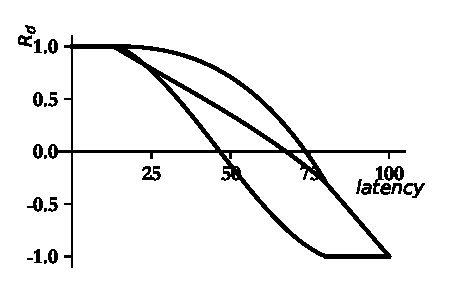
\includegraphics[width=\linewidth]{figures/chap03/reward_function/Rd.pdf}
  \caption{延迟奖励}
  \label{fig:Latency Reward}
\end{subfigure}%
\begin{subfigure}[t]{0.5\linewidth}
  \centering
  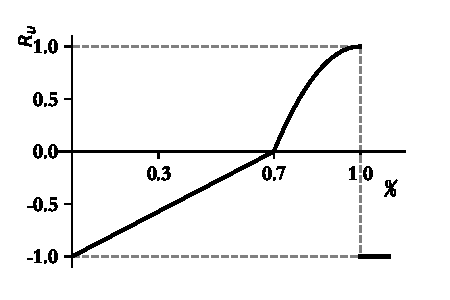
\includegraphics[width=\linewidth]{figures/chap03/reward_function/Ru.pdf}
  \caption{带宽利用率奖励}
  \label{fig:Bandwidth Utilization Reward}
\end{subfigure}

\begin{subfigure}[t]{0.5\linewidth}
  \centering
  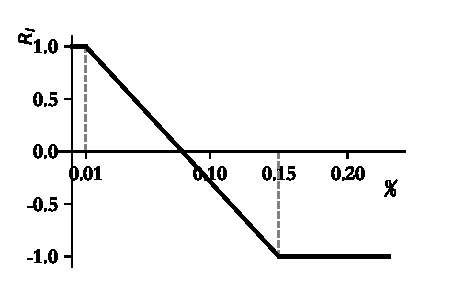
\includegraphics[width=\linewidth]{figures/chap03/reward_function/Rl.pdf}
  \caption{丢包率奖励}
  \label{fig:Loss Ratio Reward}
\end{subfigure}%
\begin{subfigure}[t]{0.5\linewidth}
  \centering
  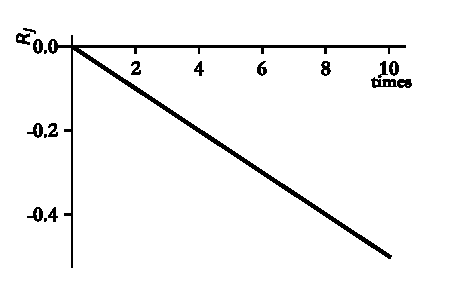
\includegraphics[width=\linewidth]{figures/chap03/reward_function/Rj.pdf}
  \caption{屏幕抖动奖励}
  \label{fig:jitter Reward}
\end{subfigure}

\caption{强化学习中的奖励函数构成}
\label{fig:reward-function}
\end{figure}





平均端到端延迟奖励 $R_d$ 将每个延迟感知敏感度曲线映射到相应的延迟奖励函数,如图\ref{fig:Latency Reward} 所示。对于超出范围的值,使用线性函数。在给定的游戏应用中,选择与其敏感性特征相对应的敏感度曲线作为奖励函数。三条曲线的表达式如式\eqref{eq:rd} 所示:
\begin{equation}
\begin{aligned}
R_{d} = 
    \begin{cases}
        1 & d < 10\\
        min\{1,0.5 \times r(d) - 1.55 \}& 10 \leq d \leq 85 \\
        max\{-1,- 0.035d +2.507\} & d > 85\\
\end{cases}
\end{aligned}
,
\label{eq:rd}
\end{equation}
其中 $r(d)$ 是式\eqref{eq:expr}所表示的内容。最终的奖励值为 $r(d)$,其中根据场景的敏感度类别选择三条曲线中的一条。

带宽利用率奖励 $R_u$ 考虑了流媒体传输流使用的带宽与总可用带宽的比率。设置传输速率过低会导致资源浪费和视频质量下降,从而造成次优的用户体验(QoE);而设置速率过高则可能导致缓冲积累,从而增加延迟。因此,带宽利用率的设计如图\ref{fig:Bandwidth Utilization Reward} 所示。当利用率低于 70\% 时,奖励线性地从最低奖励增加到 0,这作为对低带宽利用率的惩罚。同样,当利用率超过 100\% 时,会导致延迟增加、数据包丢失以及其他严重后果,从而获得最低奖励。当利用率介于 70\% 和 100\% 之间时,奖励值(大于 0)以二次函数的形式迅速增加,在 100\% 利用率时达到最大值。带宽利用率奖励函数的表达式如式\eqref{eq:ru}所示:
\begin{equation}
\begin{aligned}
R_{u} = 
    \begin{cases}
        1.429u - 1 & u < 70\%\\
        -11.111(u-1)^2 +1&  70\% \leq u \leq 100\% \\
        -1 & u > 100\%\\
    \end{cases}
\end{aligned}
,
\label{eq:ru}
\end{equation}

丢包率奖励 $R_l$ 是一个统计度量,表示在一定时间内发送的报文中未在超时前收到的比例。丢包可能导致帧的解码信息不完整,从而引发部分帧不完整、帧显示延迟以及帧序列显示错误等问题。不同帧在编码过程中有不同的优先级。在非关键帧的情况下,少量的丢包可能不会显著影响显示质量和效果,因为编解码器具备一定的错误恢复能力和抗干扰能力,例如使用前向错误纠正(FEC)技术。然而,过多的丢包将显著降低用户体验(QoE)。因此,对丢包奖励函数的设计如图\ref{fig:Loss Ratio Reward} 所示。当丢包率低于 1\% 时,奖励函数达到最大值。另一方面,当丢包率超过 15\% 时,奖励函数达到最小值。在 1\% 到 15\% 的范围内,奖励值线性下降。丢包率奖励函数的表达式如式\eqref{eq:rl} 所示:
\begin{equation}
\begin{aligned}
R_{l} = 
    \begin{cases}
        1 & l < 1\%\\
        -14.286l + 1.143&  1\% \leq u \leq 15\% \\
        -1 & l > 15\%\\
    \end{cases}.
\end{aligned}
\label{eq:rl}
\end{equation}

屏幕冻结或抖动奖励 $R_j$ 是一种衡量数据包到达间隔持续增加的次数的指标。当数据包到达间隔超过某一阈值时,屏幕冻结和抖动现象的发生概率显著增加。奖励函数通过统计发生的次数来对每次出现的现象进行惩罚。屏幕冻结与奖励之间的关系如图\ref{fig:jitter Reward} 所示,表达式为式\eqref{eq:rj}:
\begin{equation}
\begin{aligned}
R_{j} = -0.05x,
\end{aligned}
\label{eq:rj}
\end{equation}
其中$x$代表卡顿发生的次数。

最终的总奖励通过加权和求和上述四个单独的奖励组件得到,具体表达式如式\eqref{eq:total_reward}:
\begin{equation}
\begin{aligned}
R = \alpha_1 R_d + \alpha_2 R_u + \alpha_3 R_l + \alpha_4 R_j,
\end{aligned}
\label{eq:total_reward}
\end{equation}
其中,$\alpha_1, \alpha_2, \alpha_3, \alpha_4$ 是在训练过程中调整的超参数。

\subsection{场景敏感性类别确定} \label{sec-cat}
使用敏感度曲线进行强化学习中的第三个挑战是确定内容的敏感性并选择适当的曲线。可以通过统计分析,包括时间感知信息(TI)和空间感知信息(SI),来确定场景的敏感性类别。

TI 和 SI 是 ITU-R BT.1788 标准中的概念 \cite{yang2014comparison}。这些指标反映了视频流的视觉和帧特性。



TI 可以反映视频帧的时间变化。通常,运动较多的场景倾向于具有较高的 TI 值。高运动的游戏通常需要快速响应和低延迟。这些游戏通常包括第一人称射击(FPS)游戏和动作类游戏。TI 计算连续帧中每个像素在相同位置的差异,并计算标准差,然后选择最大值作为 TI,如式\eqref{eq:TI}:
\begin{equation}
\begin{aligned}
TI = \max_{t}\{std_{space}[M_n(i,j)]\},
\end{aligned}
\label{eq:TI}
\end{equation}
其中 $M_n(i,j)$ 表示第 $n$ 帧和第 $n-1$ 帧在位置 $(i,j)$ 处的像素差异。

SI 可以反映视频帧的空间细节。通常,更复杂和精细的场景会具有更高的 SI 值。例如,复杂的游戏场景通常包括塔防、策略游戏和集换式卡牌游戏(CCG),这些游戏具有视觉上复杂的图形,能够提供沉浸式的体验。SI 的计算方法是将 Sobel 滤波器应用于每一帧的亮度通道,之后进行归一化处理,最后计算在时间段内的最大标准差,如式\eqref{eq:SI}:
\begin{equation}
\begin{aligned}
SI= \max_{t}\{std_{space}[\mathrm{Sobel}(F_n)]\},
\end{aligned}
\label{eq:SI}
\end{equation}
其中,$F(n)$ 表示第 $n$ 帧,Sobel 算子是一种滤波器,它通过计算像素与其相邻像素之间灰度值的加权差异来识别边缘。

\begin{figure} [ht]
\centering
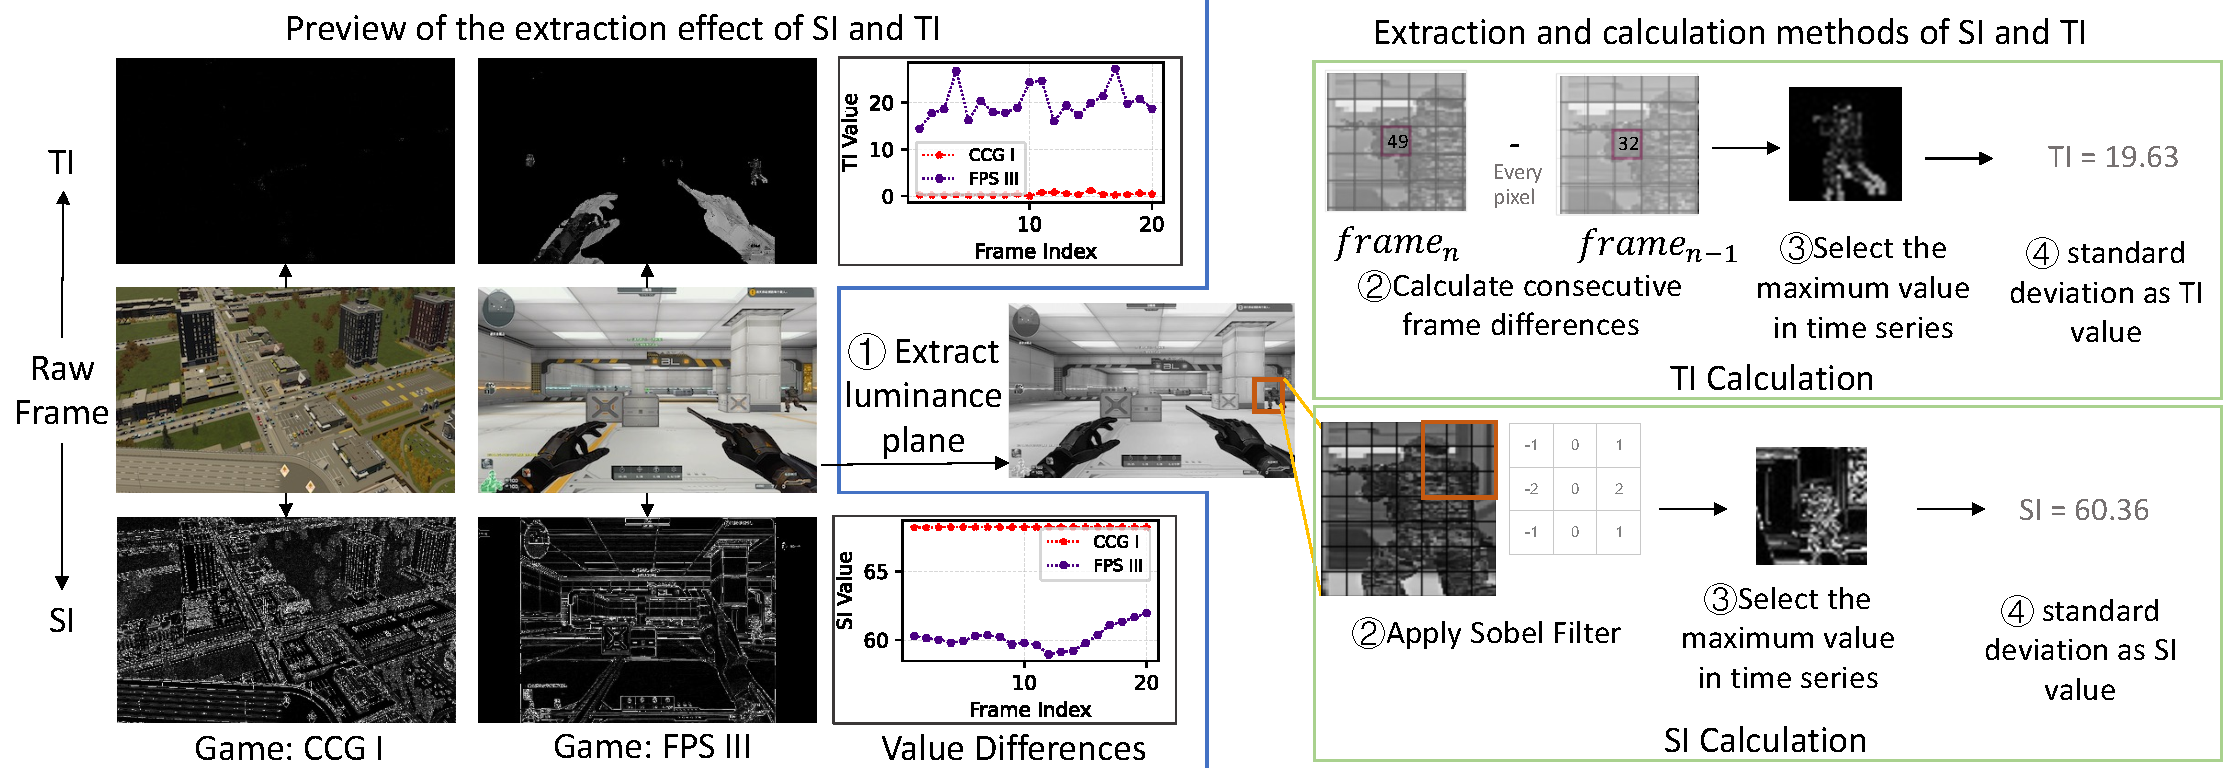
\includegraphics[width=\textwidth]{figures/chap03/intra_schematic_diagram.pdf} 
\caption{两款不同视频游戏的TI和SI提取结果的预览}
\label{fig_intra_schematic_diagram}
\end{figure}

图\ref{fig_intra_schematic_diagram}展示了来自两个场景的随机帧,并附有相应的灰度图像,这些图像映射了空间感知信息(SI)和时间感知信息(TI)值。TI 作为内容变化的指示器,使得 CCG I 由于内容变化较小,呈现出主要是黑色的图像。相反,FPS III 由于内容变化显著,展示了明显的视觉差异。SI 作为空间细节的指示器,在应用 Sobel 算子提取灰度图像时,突出了显著的边缘轮廓。特别是在视觉复杂的帧中,如 CCG I,游戏的场景内容相较于 FPS III 显得更为复杂。通过比较两款游戏中 SI 和 TI 的值差异,可以看出 CCG I 的 SI 值高于 FPS III,而 TI 值较低。此外,CCG I 的波动性较小,FPS III 则波动较大。这一观察结果强调了如何通过 SI 和 TI 度量有效捕捉并反映游戏属性和敏感性特征。

然而,SI 和 TI 的统计值并未明确表现出与游戏延迟敏感性之间的单调关系。为了解决这一问题,本章节采用了无监督聚类方法 K-Means,将数据分为三类,每一类分别表示不同程度的延迟敏感性。这种分类是基于数据与已知延迟敏感性游戏的接近程度进行的。

\section{场景需求可感知传输系统实现与部署}
超低延迟实时通信模拟器: OpenNetLab \cite{eo2022opennetlab} 提供了一个基于 AlphaRTC 的开放平台,用于快速验证基于强化学习的实时通信速率控制算法。本实验对 OpenNetLab 的 gym 模拟器进行了修改,使其适应云游戏场景,包括调整了模拟器的端到端延迟范围,以适应超低延迟需求,并增加了对帧间到达时间间隔(Frame Inter-Arrival Time)的测量能力,使得RL代理能够获得云游戏中特有状态信息,以便与 AlphaRTC 系统的常规系统状态反馈进行配合,

部署强化学习算法:本实验基于 Stable-Baselines3 \cite{stable-baselines3} 和 ReCoCo \cite{markudova2023recoco} 构建了强化学习框架。该框架支持快速构建具有自定义空间和动作的 Actor-Critic 算法,并支持低延迟推理。该框架还集成了多种训练策略,可以快速调用以验证其效果。

设置训练参数:对于式\eqref{eq:total_reward} 中的超参数 $\alpha$,本实验从相等权重开始,通过训练和与相应影响因素的平衡来确定最佳参数。对于状态空间中历史状态的长度,本实验参考了 Aurora \cite{markudova2023recoco} 并根据训练奖励的结果进行了微调。

提取 TI 和 SI 信息: 本实验新增了一个 SI 和 TI 计算模块,以从视频流中获取统计信息。基于已知的游戏敏感度类型,本实验进行了离线分类,并选择了相应的敏感度算法。

相关的算法和模拟系统部署在了一台高性能计算服务器上,配备Intel Xeon Silver 4210 CPU @ 2.20GHz,并搭载4张 NVIDIA Tesla V100S GPU显卡。
\section{实验评估方法与实验结果}
\subsection{实验评估方法设计}
数据集:为了评估Sense方法对用户体验质量(QoE)的改进,实验使用了 OpenNetLab 提供的在不同条件下的网络轨迹。这些轨迹包含了异构网络链路类型,包括有线、4G 和 5G,不同的带宽吞吐量条件。具体的链路类型为:有线 - (12Mbps),4G - (3Mbps, 700Kbps, 500Kbps) 和 5G - (35Mbps, 12Mbps, 900Kbps)。这些带宽链路的平均带宽、抖动标准差、带宽变化均值以及可模拟的总时长统计信息如表\ref{tab:bandwidth_variation}所示。

\begin{table}[ht]
    \caption{不同网络条件下的带宽和变化情况}
    % \renewcommand\arraystretch{1}
    \centering
    \resizebox{\columnwidth}{!}{%
    \begin{tabular}{@{}ccccc@{}}
    \toprule
    网络链路 & 平均带宽 (Kbps) & 抖动标准差 (Kbps) & 带宽变化均值 (Kbps) & 总时长 (秒) \\ \midrule
    WIRED\_35Mbps & 35258.76 & 3202.53 & 657.34 & 61.3 \\ 
    5G\_13Mbps   & 17315.63 & 1617.53 & 327.55 & 60.7 \\
    5G\_12Mbps   & 11644.95 & 4663.19 & 399.03 & 61.0 \\ 
    5G\_900Kbps  & 862.67   & 97.20   & 133.98 & 57.6 \\
    4G\_3Mbps    & 3019.52  & 459.90  & 57.06  & 60.8 \\ 
    4G\_700Kbps  & 678.61   & 253.62  & 165.30 & 106.6 \\ 
    4G\_500Kbps  & 497.96   & 200.42  & 124.16 & 106.0 \\ \bottomrule
    \end{tabular}
    }
    \label{tab:bandwidth_variation}
\end{table}

其中具体参数的计算如式\eqref{eq:avg_bandwidth},式\eqref{eq:standard_deri}和式\eqref{eq:deri_band_avg}所示:
\begin{equation}
\begin{aligned}
\text{平均带宽} \mu = \frac{\sum_{i=1}^{n} capacity_i \times duration_i}{\sum_{i=1}^{n} duration_i},
\end{aligned}
\label{eq:avg_bandwidth}
\end{equation}
\begin{equation}
\begin{aligned}
\text{抖动标准差} = \sqrt{\frac{\sum_{i=1}^{n} duration_i \times (capacity_i - \mu)^2}{\sum_{i=1}^{n} duration_i}}
\end{aligned},
\label{eq:standard_deri}
\end{equation}
\begin{equation}
\begin{aligned}
\text{带宽变化均值} = \frac{\sum_{i=1}^{n-1} |capacity_i - capacity_{i+1}| \times duration_i}{\sum_{i=1}^{n-1} duration_i}
\end{aligned}.
\label{eq:deri_band_avg}
\end{equation}
其中,$capacity_i$代表$i$时刻的带宽容量,$duration_i$代表模拟中的时刻$i$。

与基线算法的比较:本章节将Sense算法与 GCC 和 ReCoCo 的 QoE 实验结果进行了比较。

\begin{itemize}
    \item GCC算法 \cite{carlucci2016analysis}:GCC 算法结合了基于丢包的控制器和基于延迟的控制器,是 WebRTC 中默认的速率控制方法。它在低延迟场景下提供了稳定的连接,并能够较好地适应不同的网络状况。
    
    \item ReCoCo \cite{markudova2023recoco}:ReCoCo 是一种利用强化学习技术的拥塞控制算法,能够在复杂网络条件下实现超低延迟优化。
\end{itemize}


性能指标:本章节使用QoE作为衡量最终算法改进的指标。QoE 包括两个方面:延迟和视觉质量。
\begin{itemize}
    \item 延迟:通过MTP延迟 $L_{MTP}$ \cite{alhilal2022nebula} 进行评估,该指标衡量从用户执行操作(如键盘按键或鼠标移动)到操作结果在屏幕上显示所需的帧时间延迟。MTP延迟所对应的QoE分数可以使用式\eqref{eq:expr} 中的延迟感知敏感度函数 $r(d)$ 进行计算。
    
    \item 视觉质量:由流畅度和平滑度组成。流畅度衡量显示帧的连续性,避免因丢包和接收超时导致的帧丢失、冻结或抖动。在固定时间段内屏幕冻结的次数记为 $J$,每次冻结或抖动都会作为 QoE 的惩罚分数。平滑度评估显示帧的量化级别和分辨率,可通过编码比特率计算。通过使用式\eqref{eq:logsend} 将编码比特率 $s$ 归一化到 $[0, 5]$,以确保发送速率和延迟对 QoE 的贡献相等,归一化后的值记为 $R_{slog}(s)$。
\end{itemize}


一段时间内的平均 QoE 可以通过式\eqref{eq:qoeeva}计算:
\begin{equation}
\begin{aligned}
    QoE = 0.5 * r(L_{MTP})  + 5 * R_{slog}(s) - 0.25 * J  .
\end{aligned}
\label{eq:qoeeva}
\end{equation}

游戏敏感性分类通过 K-Means 聚类算法进行评估,并通过分类准确率作为聚类算法的评价指标。

\subsection{用户体验评估实验结果}
总体 QoE 增益:本实验使用式\eqref{eq:qoeeva} 计算了算法的最终 QoE,所有相应的结果列在表\ref{tab:exp_results} 中。

% Please add the following required packages to your document preamble:
% \usepackage{booktabs}
% \usepackage{multirow}
\begin{table*}[!ht]
\caption{Sense的QoE实验结果与其他方法对比}
\resizebox{\linewidth}{!}{%
\begin{tabular}{@{}cccccccccc@{}}
\toprule
网络条件 & 游戏类型分类 & 方法 & 平均延迟 & 尾部延迟 (95\%) & 平均 r($L_{MTP}$) & 平均发送速率(Kbps) & $R_slog(s)$ & 抖动次数 & 最终 QoE \\ \midrule
\multirow{9}{*}{\begin{tabular}[c]{@{}c@{}}高吞吐量\\      ($\geq$ 10Mbps)\end{tabular}} & \multirow{3}{*}{高敏感度} & ReCoCo               & 50.501          & 101.166             & 2.802             & 4748.340               & 4.610    & 6            & 1.728          \\
                                                                                                      &                            & GCC                  & 53.776          & 130.871             & 2.563             & 1926.600               & 3.935    & 3            & 1.687          \\
                                                                                                      &                            & \textbf{Sense(提出方法)} & 50.600          & 102.690             & 2.794             & 4379.535               & 4.549    & 3            & \textbf{1.898} \\ \cmidrule(l){2-10} 
                                                                                                      & \multirow{3}{*}{中敏感度}    & ReCoCo               & 50.501          & 101.166             & 3.739             & 4748.340               & 4.610    & 6            & 1.962          \\
                                                                                                      &                            & GCC                  & 53.776          & 130.871             & 3.621             & 1926.600               & 3.935    & 3            & 1.952          \\
                                                                                                      &                            & \textbf{Sense(提出方法)} & 50.600          & 101.000             & 3.736             & 2795.595               & 4.214    & 1            & \textbf{2.175} \\ \cmidrule(l){2-10} 
                                                                                                      & \multirow{3}{*}{低敏感度}       & ReCoCo               & 50.501          & 101.166             & 4.424             & 4748.340               & 4.610    & 6            & 2.133          \\
                                                                                                      &                            & GCC                  & 53.776          & 130.871             & 4.292             & 1926.600               & 3.935    & 3            & 2.119          \\
                                                                                                      &                            & \textbf{Sense(提出方法)} & 51.726          & 105.333             & 4.376             & 4582.741               & 4.583    & 0            & \textbf{2.490} \\ \midrule
\multirow{9}{*}{\begin{tabular}[c]{@{}c@{}}低吞吐量\\      (\textless 10Mbps)\end{tabular}}     & \multirow{3}{*}{高敏感度} & \textbf{ReCoCo}      & 53.771          & 110.143             & 2.563             & 237.945                & 2.371    & 4            & \textbf{1.234}          \\
                                                                                                      &                            & GCC                  & 177.772         & 1277.680            & 1.000             & 186.950                & 2.190    & 2            & 0.923          \\
                                                                                                      &                            & Sense(提出方法)          & 66.761          & 210.250             & 1.720             & 277.849                & 2.487    & 3            & 1.114          \\ \cmidrule(l){2-10} 
                                                                                                      & \multirow{3}{*}{中敏感度}    & ReCoCo               & 53.771          & 110.143             & 3.622             & 237.945                & 2.371    & 4            & 1.498          \\
                                                                                                      &                            & GCC                  & 177.772         & 1277.680            & 1.000             & 186.950                & 2.190    & 2            & 0.923          \\
                                                                                                      &                            & \textbf{Sense(提出方法)} & 60.397          & 111.000             & 3.373             & 271.060                & 2.468    & 2            & \textbf{1.585} \\ \cmidrule(l){2-10} 
                                                                                                      & \multirow{3}{*}{低敏感度}       & \textbf{ReCoCo}      & 53.771          & 110.143             & 4.292             & 237.945                & 2.371    & 4            & \textbf{1.666}          \\
                                                                                                      &                            & GCC                  & 177.772         & 1277.680            & 1.000             & 186.950                & 2.190    & 2            & 0.923          \\
                                                                                                      &                            & Sense(提出方法)          & 67.640          & 220.200             & 3.533             & 230.204                & 2.346    & 2            & 1.595          \\ \bottomrule
\end{tabular}
}
    \label{tab:exp_results}
\end{table*}

实验结果分别展示了高带宽链路和低带宽链路下的结果,因为云游戏通常更倾向于使用高带宽连接。对于具有不同延迟敏感度的游戏,根据其相应的敏感度曲线绘制 QoE 结果。本章的方法与 GCC 和另一种基于强化学习的方法 ReCoCo 进行了比较。在高敏感度游戏中,本章节提出的方法在延迟方面优于 GCC,并且相比 ReCoCo 方法,虽然延迟略高,但对 QoE 的影响可以忽略不计。这种改进显著减少了屏幕卡顿的发生,从而提高了 QoE 得分。

\begin{table}[!ht]
\centering
\caption{游戏的 SI 和 TI 使用 K-Means 方法进行分类的结果}
\renewcommand\arraystretch{1.25}
\begin{tabular}{@{}ccccc@{}}
\toprule
游戏 & TI & SI & K-means分类 & 正确分类 \\ \midrule
3D-RPG I           & 8.10  & 48.73  & 高敏感度          & 是                    \\
TPS I              & 18.42 & 55.39  & 高敏感度          & 是                    \\
\textbf{FPS III}   & 18.22 & 67.94  & 高敏感度          & 是                    \\
FPS IV             & 17.69 & 71.55  & 高敏感度          & 是                    \\
\textbf{FPS II}    & 16.55 & 72.05  & 高敏感度          & 是                    \\
\textbf{CCG I}     & 2.12  & 74.63  & 低敏感度           & 是                    \\
Sport III          & 11.29 & 77.00  & 低敏感度           & 否 (中敏感度)                   \\
3D-RPG II          & 10.31 & 80.21  & 低敏感度           & 是                    \\
A-RPG I            & 4.03  & 81.97  & 低敏感度           & 是                    \\
MMORPG II          & 14.02 & 84.21  & 低敏感度           & 是                    \\
MMORPG I           & 21.34 & 86.12  & 低敏感度           & 是                    \\
\textbf{MOBA I}    & 3.40  & 87.00  & 低敏感度           & 是                    \\
\textbf{MOBA II}   & 3.74  & 87.51  & 低敏感度           & 是                    \\
FPS I              & 27.74 & 89.25  & 低敏感度           & 否 (高敏感度)
                        \\
Casual III         & 10.73 & 91.49  & 中敏感度          & 是                    \\
Casual II          & 8.39  & 92.64  & 中敏感度          & 是                    \\
\textbf{Sport I}   & 11.76 & 103.32 & 中敏感度          & 是                    \\
\textbf{2D-RPG I}  & 8.13  & 108.18 & 中敏感度          & 是                    \\
\textbf{2D-RPG II} & 17.33 & 119.28 & 中敏感度          & 是                    \\ \bottomrule
\end{tabular}
\label{tab_cat_gor}
\end{table}

场景敏感度分类: 本实验通过分析游戏平台上每款游戏的动态视觉效果,对 19 款游戏进行了测试。对于每款游戏大约 600 秒的数据,实验逐帧计算了 SI(空间信息)和 TI(时间信息)值,并求取其平均值。基于 SI 和 TI 的平均值,实验使用 K-Means 方法 \cite{ahmed2020k} 进行了聚类。分类结果如表\ref{tab_cat_gor}所示。对于剩余的游戏,实验基于先前测量的游戏作为基准,确定了最终的敏感度标签。在 19 款游戏和场景中,分类结果显示仅有两款游戏的敏感度标签不匹配,分类准确率达到了 89.4\%。






训练过程中的奖励函数累计值及运行性能如图\ref{fig-evaluation-result}所示。图\ref{fig-reward-func}显示了训练过程中累计奖励的变化。图\ref{fig-band-util}、\ref{fig-latency-cdf}和\ref{fig-jitter-times}展示了算法运行过程中收集的状态参数。图\ref{fig-band-util}显示了在相同带宽下发送速率的变化,结果表明Sense算法与 ReCoCo 相似,并且超越了 GCC。图\ref{fig-latency-cdf}显示了数据包延迟的累积分布函数(Cumulative Distribution Function,CDF),高敏感度和中敏感度的低延迟表现优于 ReCoCo,而低敏感度则保持在不敏感范围内。图\ref{fig-jitter-times}展示了Sense算法在固定时间段内能实现更少的抖动次数。

\begin{figure}[!ht]
\centering
\begin{subfigure}[t]{0.5\linewidth}
  \centering
  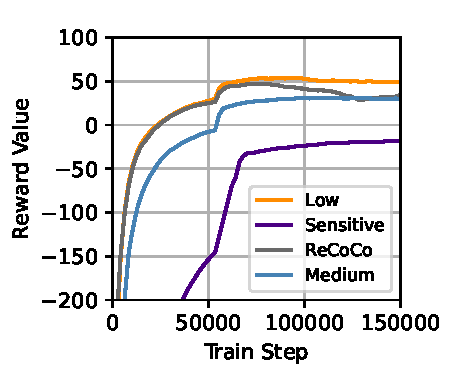
\includegraphics[width=\linewidth]{figures/chap03/evaluation_plots/reward_value.pdf}
  \caption{训练过程中的奖励值累计}
  \label{fig-reward-func}
\end{subfigure}%
\begin{subfigure}[t]{0.5\linewidth}
  \centering
  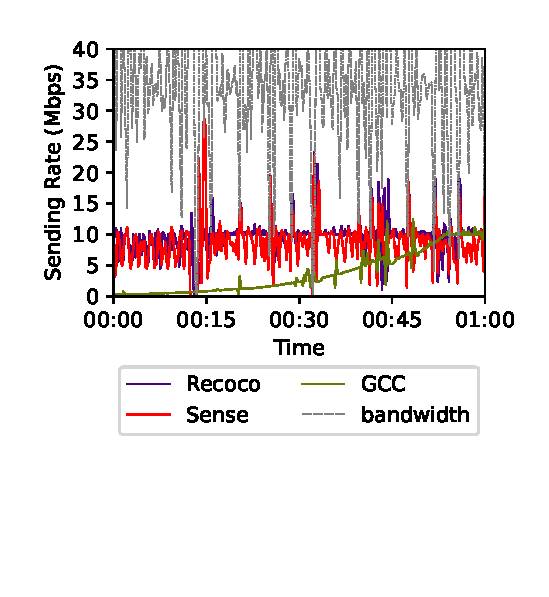
\includegraphics[width=\linewidth]{figures/chap03/evaluation_plots/bandwidth.pdf}
  \caption{带宽利用率}
  \label{fig-band-util}
\end{subfigure}

\begin{subfigure}[t]{0.5\linewidth}
  \centering
  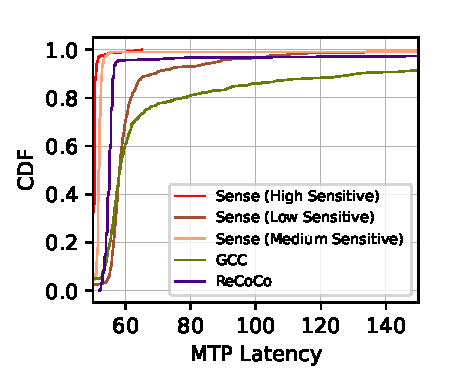
\includegraphics[width=\linewidth]{figures/chap03/evaluation_plots/cdf_delay.pdf}
  \caption{延迟的累积分布函数 (CDF)}
  \label{fig-latency-cdf}
\end{subfigure}%
\begin{subfigure}[t]{0.5\linewidth}
  \centering
  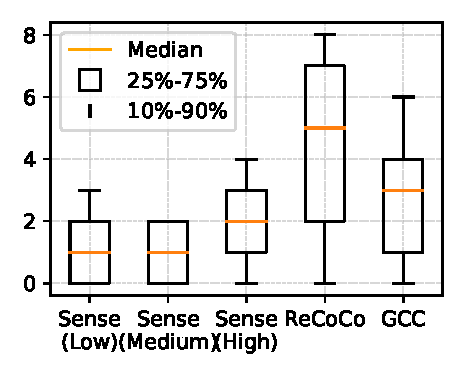
\includegraphics[width=\linewidth]{figures/chap03/evaluation_plots/jitter_times.pdf}
  \caption{抖动次数}
  \label{fig-jitter-times}
\end{subfigure}

\caption{训练过程中的奖励函数累计值及运行性能}
\label{fig-evaluation-result}
\end{figure}

 

\subsection{设计方案局限性讨论}
如果一款游戏场景被错误分类,将会对性能带来怎样的影响?为了进一步分析错误分类对系统性能的影响,本实验继续进行了两个案例研究,分别探讨高敏感度场景被误分类为低敏感度以及低敏感度场景被误分类为高敏感度时的 QoE 变化情况。实验结果如表\ref{miscals}所示。如果高敏感度场景被误分类为低敏感度,会导致显著的 QoE 损失,几乎抵消了 Sense 的优势;但若低敏感度场景被误分类为高敏感度,导致“过度满足”的延迟 QoE,但略微降低了图像质量并增加了卡顿。尽管这些情况的发生会降低QoE,但最差的结果也不会低过最低基准能够达到的QoE;且这些是极端的误分类情况,第一个案例代表了最差的结果。这些情况发生的概率也非常罕见。
\begin{table}[ht]
\centering
\caption{敏感度误分类对QoE的影响}
\renewcommand\arraystretch{1.25}
\resizebox{\columnwidth}{!}{%
\begin{tabular}{@{}cccc@{}}
\toprule
\textbf{案例} & \textbf{QoE} & \textbf{相较于正确分类的 QoE} & \textbf{相较于最低基准的 QoE} \\ \midrule
应为高敏感度但被误分类为低敏感度 & 1.84  & -7.43\%                     & +0.54\%                     \\ 
应为低敏感度但被误分类为高敏感度 & 2.30  & -0.90\%                     & -0.04\%                     \\ \bottomrule
\end{tabular}
}
\label{miscals}
\end{table}

\section{本章小结}
本章节提出了 Sense,一种基于强化学习的用户时延敏感度可感知的场云游戏场景传输速率控制算法。通过测量和用户 MOS 实验,利用不同游戏在延迟感知敏感度上的差异,Sense 在强化学习框架中重构了状态和奖励空间。这使得可以根据游戏敏感度的不同类别,对延迟和视觉质量权衡采取差异化策略。实验结果表明,Sense 提高了视频流的流畅性,将总体用户体验质量(QoE)提升了 9.8\% 至 16.7\%,并以 89.4\% 的准确率完成了游戏敏感度分类。

















% !TeX root = ../thuthesis-example.tex

\chapter{具备策略库的网络任务规划范式设计}
\section{本章序言}
在网络领域,有许多重要的任务,包括拥塞控制、可变比特率控制和梯度压缩任务,这些任务在过去几十年中积累了众多有效的方法。例如,在拥塞控制任务中,有基于简单规则的算法(如 Cubic \cite{ha2008cubic},基于丢包的算法,以及 BBR \cite{cardwell2016bbr},基于带宽-延迟积的算法),也有基于人工智能的方法,如强化学习(例如 Sage\cite{yen2023computers})或在线学习(例如 PCC Vivace\cite{dong2018pcc})。这些任务涉及许多策略,形成了各自的“策略库”,这些策略库是经过数十年努力和不断完善的结果,由无数学者创造,最终形成了一套可以应用于各种场景的强大算法集合。大多数方法基于不同的设计原则,具有不同的性能和适用性,能够适应不同的网络环境和需求。部分算法的统计如表\ref{table_task_algo}所示。

然而,在传统的网络传输控制范式中,大多数连接在建立时采用固定的控制策略。以拥塞控制为例:在绝大多数Linux个人主机上,默认使用Cubic算法,除非用户手动切换算法。即便在数据中心,通常也会配置固定策略以确保服务的稳定性,所有连接都会使用单一的控制方法。这个经典范式的缺点在于依赖于单一策略,即使网络特性可能更适合采用不同的策略,从而缺乏多样性。事实上,由于每种拥塞控制算法设计原则的不同,不论一个策略多么强大,它都会因为设计上的局限性而表现出局部性和偏差,无法涵盖所有网络条件,在某些场景下可能会陷入局部最优解。

为了避免陷入这种困境,最直观的方法是根据网络状况手动为每种情况选择一个策略。然而,这种做法的成本远大于其收益。在过去几十年里,一些研究致力于转变这种传统范式。例如,Remy \cite{winstein2013tcp} 通过利用关于网络的先验知识或假设,旨在生成一种拥塞控制策略。Sage \cite{yen2023computers} 试图通过离线强化学习来学习各种算法的“优势”,从而在大多数场景中表现出优于其他算法的效果。另一方面,Antelope \cite{zhou2022machine} 提出了一个避免设计“千篇一律”算法的系统,而是根据情况在“最适合”的控制算法之间切换。尽管这些范式具有开创性,但它们仍然受到个别算法性能的局限性或从多种算法中选择的瓶颈所制约。

然而,近年来,大型语言模型(Large Language Models,LLMs)的出现为转变这一旧有范式提供了新的机遇。许多研究证明,LLMs在环境感知理解、规划和决策方面具备强大的能力,这一点通过LLMs代理的崛起得到了体现,并且它们已经在工具规划中得到了应用。此外,通过适当的微调和设计技术,这些LLMs还可以在特定领域进一步提升其性能。LLMs所展现出的决策能力也表明,它们有潜力感知网络环境、理解应用需求,并做出相应的规划。

受到此启发,本工作提出了一种新的范式,在这种范式中,对于任何类型的网络决策任务,预训练的LLMs 根据网络状况从策略库中选择“最适合”的策略,从而实现动态的宏观层级策略切换,增强算法选择的适应性。

构建这一范式面临以下挑战:

\begin{itemize} \item \textbf{改变范式及LLM对网络状况的感知。}目前的网络控制算法和协议缺乏在连接建立过程中切换方法的能力,因此需要重新定义工作流程,增加一个切换控制策略的步骤。此外,网络系统需要增强感知趋势、通用信息和应用层需求的能力。

\item \textbf{网络策略决策的独特性。}常见的规划任务通常在静态环境中运行,任务可以通过链式思维(Chain-of-Thought)等技术进行分解,并通过即时反馈(如人工反馈或环境反馈)加以解决。然而,在网络任务中,决策难以明确分解,且反馈在决策之后延迟出现。此外,环境是非确定性的,存在概率性变化。因此,LLM在网络场景中的规划能力与传统的LLM规划方法有所不同。

\item \textbf{LLM获取网络决策经验的问题。}尽管预训练的LLM拥有丰富的知识,但它们仍然缺乏在网络策略选择和决策中做出有效选择的能力。目前所获得的知识尚不足以使LLM在这一背景下始终做出有价值的决策。 
\end{itemize}

针对上述挑战,本工作的主要设计思路包括一个新的范式,该范式结合了使用特定技术微调的LLM和修改后的系统工作流程。

为了使模型具备选择策略的能力,该工作将策略规划问题视为强化学习任务,并利用决策变换器(Decision Transformer)的离线强化学习框架 \cite{chen2021decision},为模型学习提供机制。该工作使用LoRA方法来训练模型中部分变量权重,并通过模型微调(Supervised Fine-Tuning,SFT)来提升规划性能。

为了感知网络趋势的变化,该工作设计了一个针对多维网络时间序列数据的自定义嵌入层,使工作能够提取任务在较长时间段内的时序语义。

此外,该工作引入了网络系统与策略规划系统之间的交互机制,使得不同的策略和算法可以在执行过程中灵活切换,以更好地适应当前状态。


\section{网络领域策略性控制的范式背景}
在网络领域,许多任务需要策略性控制,以提高网络利用率并确保质量保障。自适应码率流媒体(Adaptive Bitrate Streaming,ABR)、拥塞控制(Congestion Control,CC)和梯度压缩(Gradient Compression,GC)等任务占据了大部分网络流量,并且是关键的质量保障节点。因此,过去几十年里,针对这些领域进行了大量研究,不断引入新的方法和思想。这些研究和工程实现最终形成了一个庞大的算法库,这些算法在不同的原理和工作机制下运行。一些经典算法列在表\ref{table_task_algo} 中。

\begin{table}[htbp]
\centering
\caption{网络环境中的重要任务关键性能指标及经典控制策略}
\resizebox{\columnwidth}{!}{%
\begin{tabular}{@{}ccccc@{}}
\toprule
\textbf{任务}                                          & \textbf{关键性能指标}                                & \textbf{策略} & \textbf{原理} & \textbf{年份} \\ \midrule
\multirow{6}{*}{\textbf{自适应码率流媒体}} & \multirow{6}{*}{重缓冲、码率、平滑性} & Pensieve \cite{mao2017neural}          & 基于强化学习            & 2017          \\
                                                       &                                              & Genet \cite{xia2022genet}            & 基于强化学习            & 2022          \\
                                                       &                                              & MPC               & 动态规划                  & 2015          \\
                                                       &                                              & BBA               & 基于缓冲区        & 2014          \\
                                                       &                                              & BOLA \cite{spiteri2020bola}             & 基于缓冲区        & 2016          \\
                                                       &                                              & NetLLM \cite{wu2024netllm}            & 基于Transformer   & 2024          \\ \midrule
\multirow{6}{*}{\textbf{拥塞控制}}           & \multirow{6}{*}{吞吐量、丢包、延迟}    & CUBIC \cite{ha2008cubic}             & 基于丢包          & 1990年代         \\
                                                       &                                              & Reno              & 基于丢包          & 1990年代         \\
                                                       &                                              & WestWood \cite{casetti2002tcp}          & 基于丢包          & 2002          \\
                                                       &                                              & BBR \cite{cardwell2016bbr}
                                                    & 带宽延迟积                 & 2015          \\
                                                       &                                              & Aurora \cite{jay2019deep}            & 基于强化学习            & 2019          \\
                                                       &                                              & Sage \cite{yen2023computers}             & 基于强化学习            & 2023          \\ \midrule

\multirow{2}{*}{\textbf{梯度压缩}}         & \multirow{2}{*}{压缩率、准确度、效率}                            & Top-K             & 稀疏化           & 2010年代        \\
                                                    
                                                       &                                              & DC2 \cite{abdelmoniem2021dc2}             & 基于延迟    &   2021            \\ \bottomrule
\end{tabular}
}
\label{table_task_algo}
\end{table}


这些任务的介绍如下:

\textbf{自适应码率:} 主要用于视频流媒体,基于实时网络状况自动调整视频质量,以确保流畅播放并优化用户体验,尤其是在带宽波动时。

\textbf{拥塞控制:} 旨在通过动态调整数据传输速率来避免网络过载,从而提高网络稳定性和效率,即使在高流量条件下也能确保良好的服务质量。

\textbf{梯度压缩:} 在模型训练过程中减少传输的梯度信息的大小,以降低通信成本并提高分布式训练的效率,通常用于训练大规模深度学习模型。

然而,由于这些方法的工作原理和设计理念不同,算法在不同网络环境中的表现也各不相同。没有单一的算法能够在所有网络条件和场景中始终表现出优越的性能。以自适应码率流媒体场景作为验证,该工作使用累积奖励值来评估算法在随机网络环境中的表现。累积奖励的计算方式如式\eqref{eq:abr_cum_reward}所示:

\begin{equation}
\begin{aligned}
    \sum_i(\alpha \cdot Rebuf_i + \beta \cdot Bitrate_i + \gamma \cdot BitrateChange_i) \cdot \frac{1}{n}
\end{aligned}
\label{eq:abr_cum_reward}
\end{equation}

较高的累积奖励值表示更好的性能。测试结果如图\ref{fig_manual_switch} 所示。该工作使用genet策略进行测试,如紫色线所示,并观察到当网络遇到波动时,会导致显著的奖励损失,从而导致累积奖励的下降。相比之下,在该工作构建的可切换系统中,使用随机选择功能随机选择的算法能够缓解对整体累积奖励的影响,如橙色线所示。基于预先手动选择和切换算法的策略表现出了最佳的累积奖励,代表了最优性能,如棕色线所示。

\begin{figure} [h!]
\centering
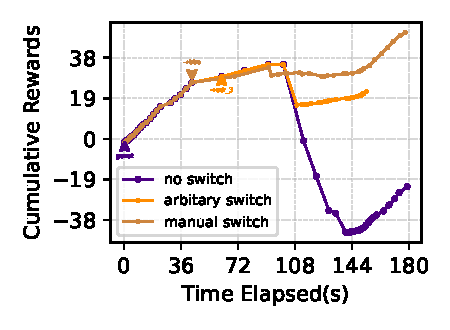
\includegraphics[width=0.5\linewidth]{figures/chap04/manual_switch_validation.pdf} 
\caption{策略切换带来的性能改变}
\label{fig_manual_switch}
\end{figure}



\section{范式更新的设计动机}
绝大多数网络任务在环境变化的情况下,仍然使用单一策略持续运行。这一直是常见的采用模式。在这种背景下,许多强大的算法得到了开发。然而,迄今为止,没有任何单一策略能够在所有网络环境中表现出色,或者在每个场景中展示最优性能,这主要是由于它们设计原理的差异。为特定条件优化的策略已经被创造出来,使得它们能够在这些特定场景中表现优异。然而,尽管通用算法可能适用于更多场景,它们通常不如针对性策略表现得那么好;相反,针对性策略可能不具有如此广泛的适用性。人们必须接受的关键观点是:策略必须在针对性优化和通用性之间找到平衡,而不可能同时实现两者的极致最优。

事实上,这个丰富且适应性强的策略库在过去几十年中通过一系列战略性进展无意间建立起来了。能否开发一种方法,利用这个库中各种策略的优势,同时避免它们的弱点?一种直观的方法是,在合适的时机从这个库中选择最适合的策略,并在必要时进行切换,如图\ref{fig_paradigm_change} 所示。图中最下方的“环境”代表客观环境的波动,在图中网络状况被分成了三段。过去的范式采用一成不变的规则,而新的范式支持在策略库中根据网络环境的变化采取切换的措施。

\begin{figure} [ht]
\centering
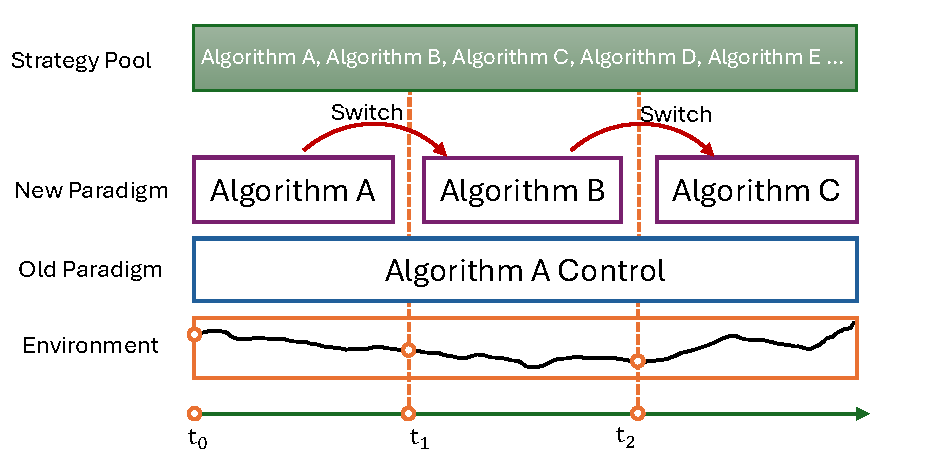
\includegraphics[width=0.7\textwidth]{figures/chap04/Paradigm_change.pdf} 
\caption{新范式利用算法库在网络环境变化时进行策略切换}
\label{fig_paradigm_change}
\end{figure}

然而,实现该工作范式将在构建时会面临下列挑战和问题:

\textbf{如何进行策略规划?} 最简单的实现和验证方法是通过手动或使用简单规则来监控和评估当前环境,然后根据策略的设计原理,从策略库中选择和配置最合适的策略。通过手动和随机切换的案例,已经证明了这种切换可以带来性能提升。这种方法适用于小规模的演示和效果验证,但显然依靠人工无法总结所有适当的切换规则,而且手动维护的成本太高。

近年来,大型语言模型的出现为转变这一旧有范式提供了新的机会。许多研究已证明,LLMs在环境感知理解、规划和决策方面具有强大的能力,正如LLM代理(LLM Agents)\cite{wang2024survey} 的崛起及其在工具规划中的应用所证明的那样。此外,通过适当的微调和设计技术,这些LLMs可以在特定领域进一步提高其性能。LLMs展示的决策能力也表明,它们有潜力感知网络环境、理解应用需求并制定合适的规划。

\textbf{为什么不使用简单的算法?} 使用基于规则的算法(如决策树)来完成策略规划,缺乏动态更新能力和应对所有条件的能力。该工作的设计期望这个范式能够基于网络环境和动态更新的策略库进行有效规划,包括算法选择和参数配置。这不仅仅是一个简单的分类或回归任务,也没有直接可映射的函数。基于规则的策略将面临与前面例子相同的问题,无法更新并识别所有可能的情况。而LLMs更擅长从人类偏好和需求理解的角度进行思考。

\textbf{为什么不让LLMs生成基于规则的策略?} 由于LLMs的幻觉问题,直接生成规划策略会导致严重的不稳定性。在工具规划工作中,LLM-ABR使用了多个验证机制来确保部分有效的答案,但对于需要高稳定性的网络任务来说,这是不可接受的。此外,直接生成基于规则的策略并不能充分利用随着时间积累起来的大量策略库。

\textbf{为什么不直接使用LLM作为策略?} 主要的限制因素是LLMs的推理延迟。LLM的推理延迟是一个显著因素,因为网络任务需要高实时性性能。如表\ref{tab:infer_latn}所示,LLM的生成延迟常常超过可接受的安全范围。在多款高性能GPU上,模型每个代词(Token)的推理速度仍然会慢于拥塞控制、自适应比特率流、梯度压缩的最高要求,尤其是当生成的代词(Token)数量较多时。类似地,直接使用LLM作为策略生成器也存在超出安全阈值的风险。


\begin{table}[ht]
\caption{大型语言模型推理的时间消耗与网络任务所需时效对比}

\resizebox{\columnwidth}{!}{%
\begin{tabular}{@{}ccccc@{}}
\toprule
项目                              & 模型         & 量化方式   & 运行GPU              & 延迟\cite{colab2023}  \\ \midrule
理论                            & Mistral-7B    & 16位        & RTX 4090(1008 GB/s)      & 14.1ms/Token               \\
理论                            & Mistral-7B    & 8位         & RTX 4090                 & \textbf{7ms/Token}         \\
实际                            & ChatGLM3-6B   & 16位        & RTX 4090(2022)           & 16ms/Token                 \\
实际                            & ChatGLM3-6B   & 16位        & V100 32GB (2017)         & 32ms/Token                 \\
实际                            & Qwen-7B       & 16位        & RTX 4090(2022)           & 19ms/Token                 \\
拥塞控制                          & /             & /              & /                        & 1$\sim$3 RTT (10$\sim$50ms) \\
自适应比特率流                   & /             & /              & /                        & 每个块 (1-5s) \\
梯度压缩                          & /             & /              & /                        & 每次迭代 \\
\bottomrule
\end{tabular}
}
\label{tab:infer_latn}
\end{table}


因此,本工作决定构建一个基于大模型的策略规划方法,该方法在一个能够切换策略的范式内运行。该方法能够有效选择和配置策略,并依赖于一个可靠的过程,在必要时动态切换策略。由于运行中的策略已经经过验证并且稳定,系统保持可靠性和鲁棒性。




\section{网络任务规划范式设计}
在确定利用大模型的决策和规划能力对于网络层面的策略做出宏观调控后,本工作致力于解决将其应用过程中的挑战。为此,本工作设计了LLM-NP(Large Language Model for Network Planning),它提供了利用大模型进行网络规划的范式。LLM-NP运行过程可以使用图\ref{fig_llmcc_design}表示。具体而言,LLM-NP的设计由网络与决策系统的策略选择和交互机制、模型规划能力的习得和调优以及模型对网络变化趋势感知和分析三个重点构成。

\begin{figure} [ht]
\centering
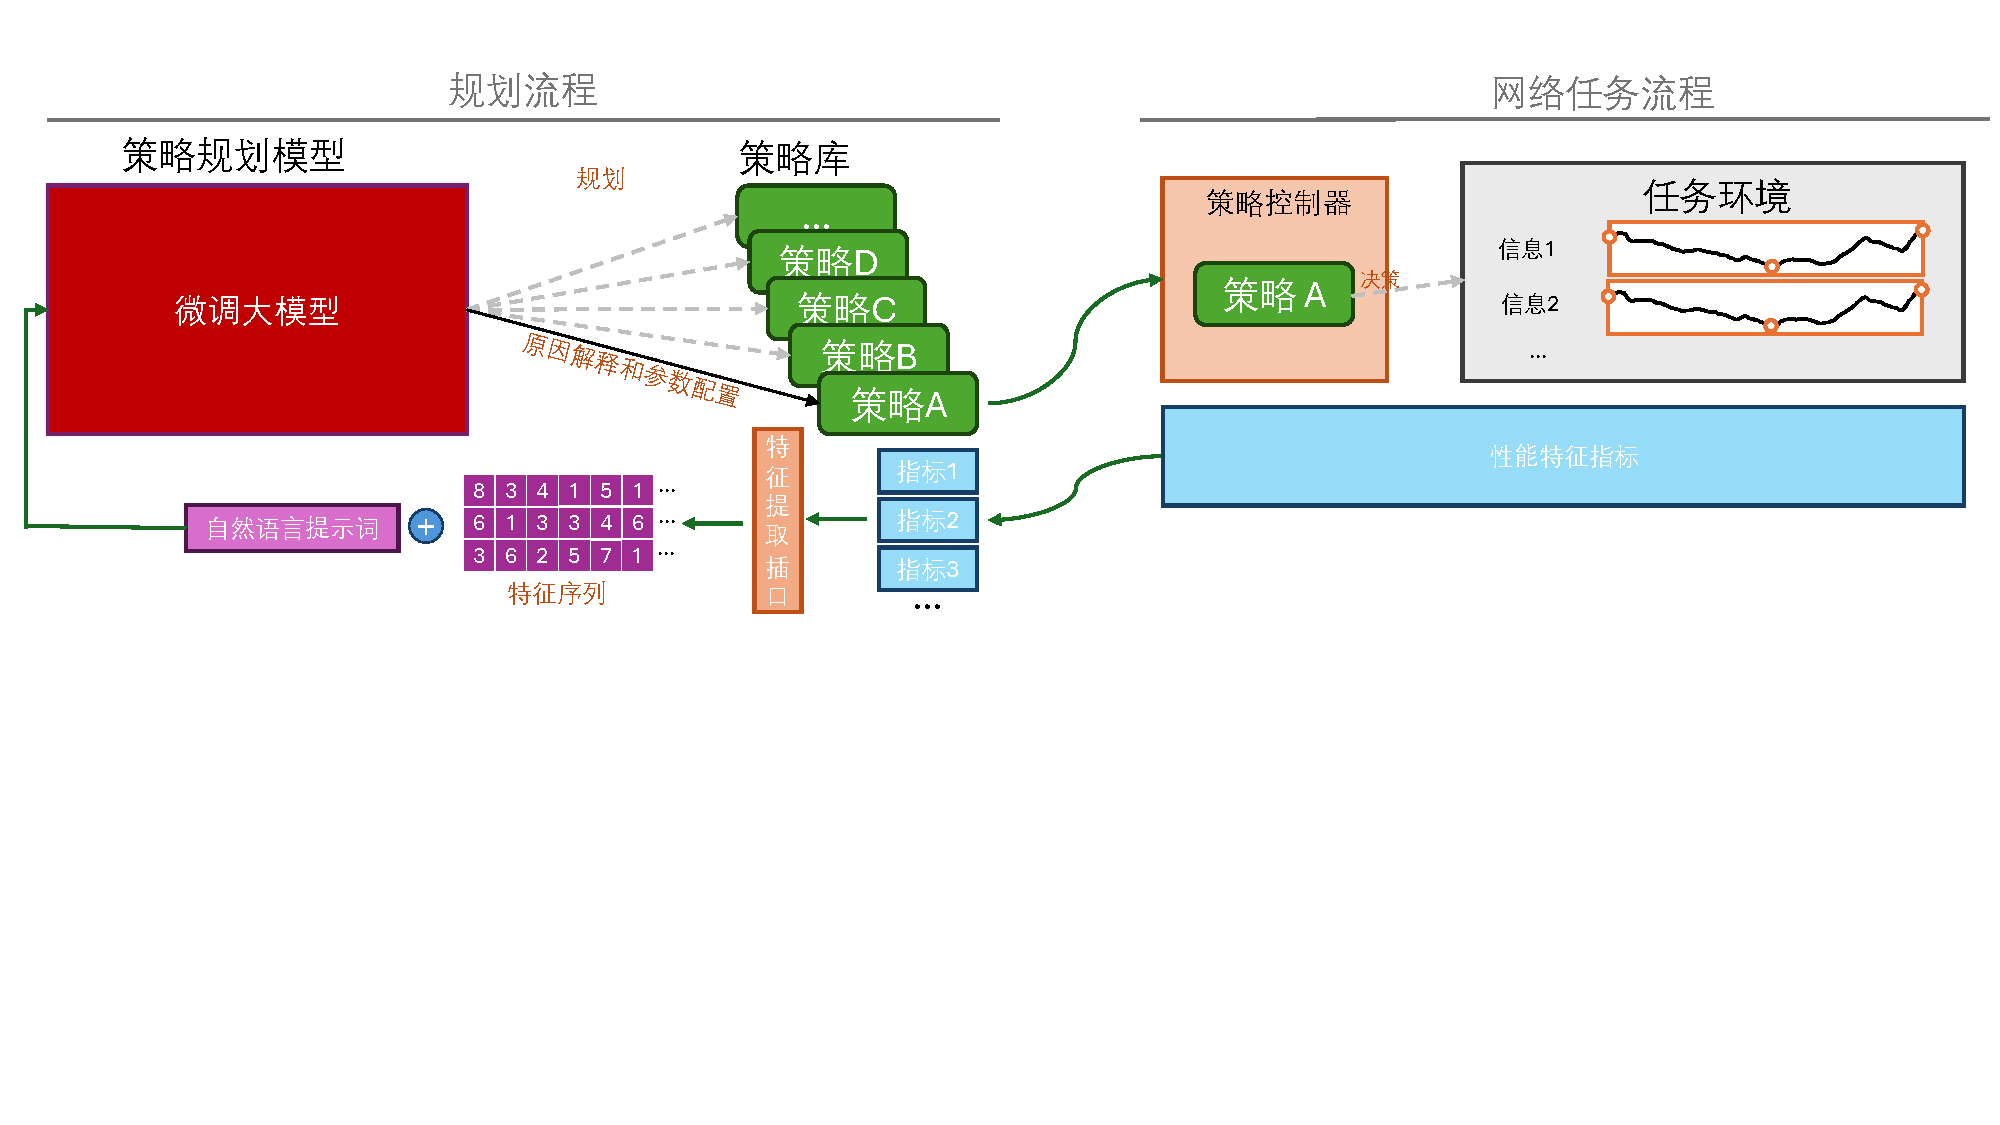
\includegraphics[width=\textwidth]{figures/chap04/design.pdf} 
\caption{网络控制策略选择范式设计概览}
\label{fig_llmcc_design}
\end{figure}


\subsection{网络与决策系统的策略选择和交互机制}
系统运行的整个流程被分为规划流程和网络任务流程。规划流程接收来自于网络任务中的指标反馈,负责在已支持的备选策略库中选择策略,根据当下和先前的网络状态做出合理的规划;而网络任务则可以是任何一个需要进行网络规划的任务。为了适配规划流程,网络任务流程也需要进行调整,以暴露出其从一个算法切换为库中其他算法、和网络状态反馈的接口,如图\ref{fig_llmcc_api}所示。以自适应码率任务为例,流媒体的发送服务器作为一个独立进程工作,并定期将网络状态和工作相关的指标(例如发送的速率、是否遇到缓冲重加载、估计带宽的信息)以网络间进程通信的方式发送给规划进程。规划进程在获得相关指标后使用LLM进行分析,并给出规划的结果,这个结果交由网络任务系统,并在网络任务系统中进行切换。

\begin{figure} [ht]
\centering
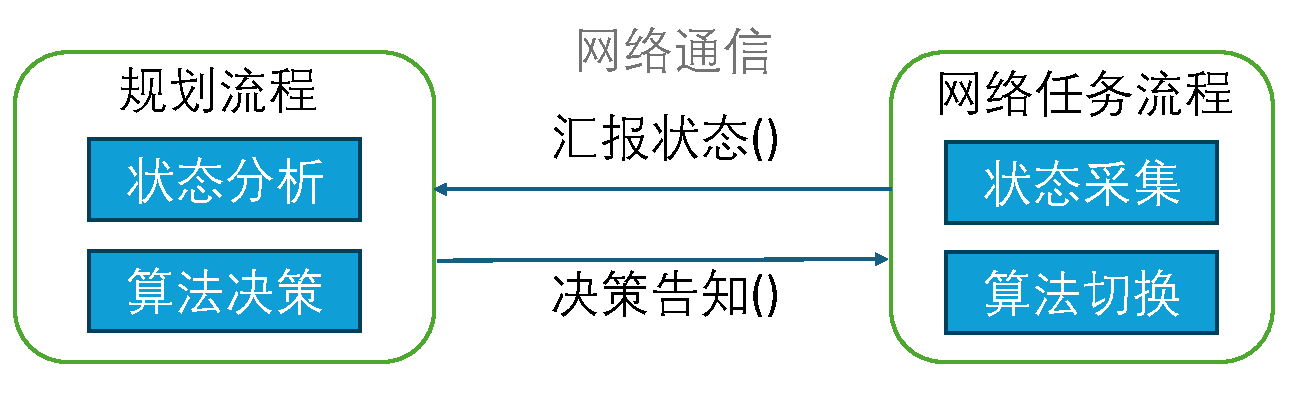
\includegraphics[width=0.65\textwidth]{figures/chap04/API.pdf} 
\caption{规划流程和网络任务流程需开放的接口和交互模式}
\label{fig_llmcc_api}
\end{figure}


这种独立流程的方式有两个好处:

(1)规划进程与网络任务进程独立运行,互不干扰。两者之间通过网络协议通信,可以建立独立的规划服务器运行规划进程,将规划进程独立运作于适合推理硬件性能的服务器上,作为中枢专为网络中心提供合适的架构。对于部份运行环境要求严苛的算法,这种运行模式避免了大模型所需的推理环境与规划进程互相冲突的局面。

(2)对要求稳定的网络任务来说,这种运行机制保证了在真实服务中避免出现系统崩溃的现象,也避免了无响应的状态:即便规划进程的推理异常或无响应,这不干扰本身设计高度稳定的网络任务进程,它将继续提供服务。即使规划进程的规划不佳,它不会造成运行的停滞或大幅下降,下限是取决于具体的策略库中的策略性能下限的。

\subsection{模型规划能力的习得和调优}
规划流程的规划能力依赖于其所使用的模型。大语言模型已经成功地向世人证明了它强大的语言、泛化和规划能力,拥有强大的预训练知识,但由于对策略库中的策略的不了解(通常在大规模预训练阶段会选用自然语言的、常识的语料库),大模型在面对网络任务时利用策略库的规划能力需要进一步微调。

\textbf{问题的建立:}网络工作的实际环境复杂多变。例如在自适应码率的任务中,网络带宽的变化是非确定性的,同时上一个传输的视频块大小会影响到后续的决策。为了简化问题,可以将环境的状态转移视为一个马尔可夫决策过程(MDP, Markov Decision Process)过程, 由网络指标所对应的状态和执行的策略规划动作,以及状态转移的概率构成。

\textbf{模型:}为了利用上预训练大模型丰富的知识,该工作决定在模型已有权重的基础上使用低秩矩阵适配的方式进一步对齐任务,通过两个低秩矩阵的相乘改变部份大模型的权重,这可以在可控的训练成本下完成模型的调优、准确率的提升和决策性能的提升。

\begin{figure} [h!]
\centering
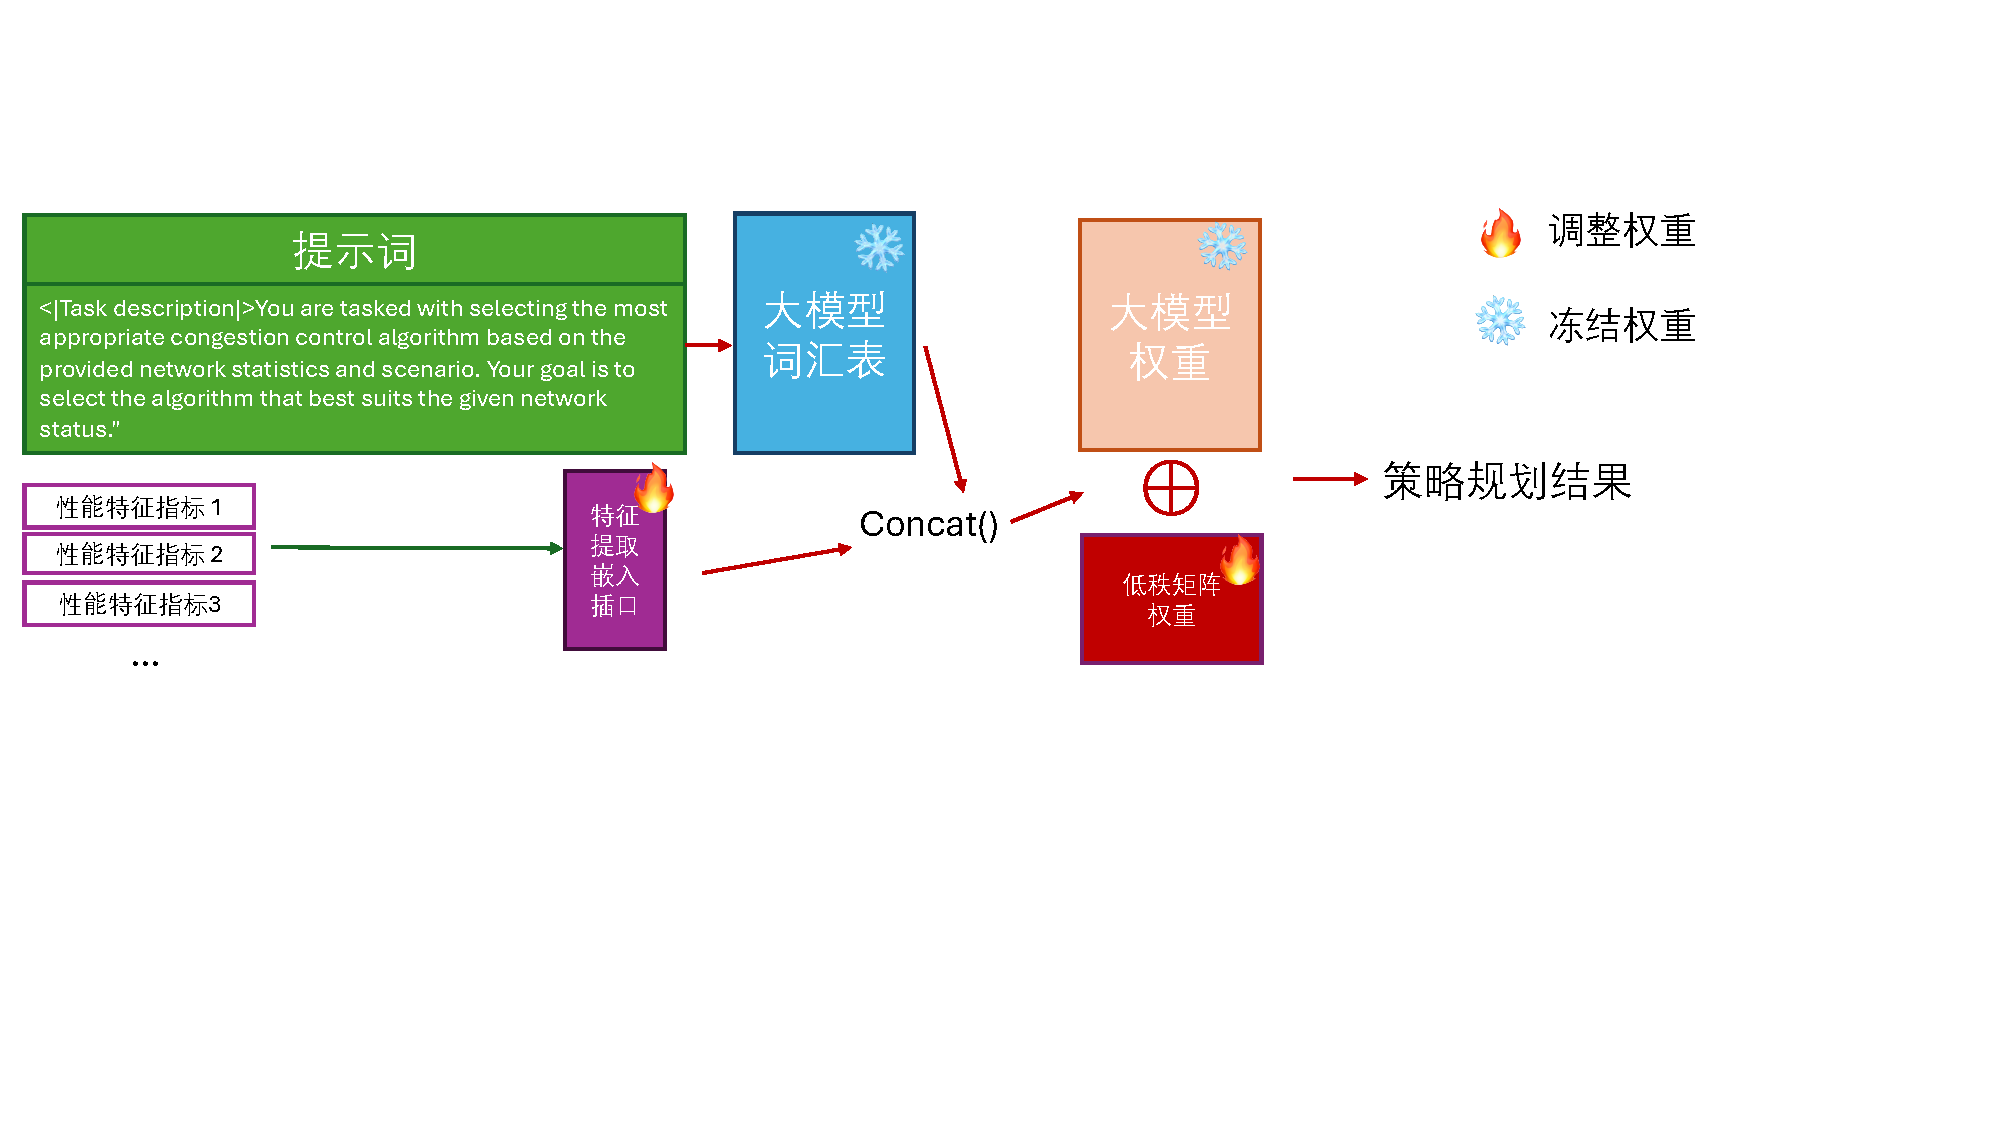
\includegraphics[width=\linewidth]{figures/chap04/model.pdf} 
\caption{LLM-NP模型的结构和权重调整情况}
\label{fig_model}
\end{figure}

\textbf{训练和学习框架:}使模型能够做出合适的策略规划决策需要在与环境交互中训练习得。解决此马尔可夫决策过程问题可以使用强化学习的方法,将任务对应的关键网络指标构成的空间视为状态空间,策略规划内容作为动作空间,并根据性能表现的结果设定奖励空间。大模型的Transformer结构使用注意力机制完成对于下一个代词(Token)的预测。在决策类任务中,Decision Transformer\cite{chen2021decision}能够提供一个适配大模型代词化输入的模型。Decision Transformer将强化学习空间中的状态(State)、动作(Action)、奖励(Reward)进行序列建模,从而给大模型符合输入要求格式、便于理解的序列,以便预测出高回报(Return)的动作。本工作使用这个方法完成前述强化问题的训练。


\textbf{数据的采集:}网络环境在运作时低容错的特性使强化学习的智能体在对应的环境中实时交互变得困难。因此使用离线的强化学习方式展开数据采集是更加合适的。离线强化学习的数据使用具体的网络任务进程给出的反馈作为数据源,并构建一个随机决策器在固定间隔内做出一个算法决策。这些决策以网络任务具体的阶段作为节点进行评估,评估方法采用任务对应的有效评估指标对一段时间内的决策效果给出可以量化的评估结果。大量这样的数据在环境中生成,然后经过一个过滤器留下评估分数最佳的前 $\alpha$\% 策略规划轨迹,作为模型的训练数据源。$\alpha $值的大小根据训练后评估实际效果、所需数据量以及工程经验综合决定,一般设置在5\%-20\%。

\textbf{训练、验证和仿真:}训练模型和验证模型使用离线数据,而仿真则在网络环境下运行和决策。训练时,进程单独运行,以损失函数值为目标优化;而仿真时,网络任务的性能指标作为评估结果直观地反馈运行结果。

具体的工作算法和流程如算法\ref{algo_proc}所示。


\begin{algorithm}
\caption{规划与网络任务控制流程}
\label{algo_proc}
\begin{algorithmic}[1]
% \STATE \textbf{输入:} 网络变化趋势嵌入接口, 预训练模型权重
% \STATE \textbf{输出:} 网络规划结果, 网络状态统计信息

\STATE \textbf{规划流程}:
\STATE 配置网络分析嵌入接口
\STATE 加载模型权重

\WHILE{接收到状态回报}
    \STATE 网络规划
    \STATE 发送网络规划结果
\ENDWHILE

\STATE \textbf{网络任务控制流程}:
\STATE 执行网络任务

\WHILE{固定粒度的时刻到达}
    \STATE 采集网络状态信息
    \STATE 发送网络状态统计信息
\ENDWHILE

\STATE \textbf{异步线程执行}:
\WHILE{收到发送结果}
    \STATE 根据规划结果开始切换算法
\ENDWHILE

\end{algorithmic}
\end{algorithm}

\subsection{模型对网络变化趋势感知}
模型对于网络变化趋势的感知和分析在强化学习的框架下将被抽象为动作、状态和奖励值。这些变量又在Decision Transformer的框架下需要抽象为符合大模型输入的序列。该工作在此过程中定义任务嵌入插口。通过任务嵌入插口,该范式支持将具体的性能指标和网络状态映射到大模型的嵌入层。无论是何种指标,每个指标经过一个多维线性层可以将低维的信息映射为大模型所需的隐藏层维度。最后,如果有多个维度的指标,将所有维度的指标连接起来,就可以形成符合大模型输入的序列。这适用于离散状态、动作和奖励空间的表示。如果空间是连续的,可以直接采用嵌入层映射到对应的维度,完成模型对网络变化趋势的感知和分析。

这样做可以实现任务规划的切换。对于不同的任务,切换对应的嵌入层就可以完成此任务的专业规划。这种方式非常灵活,就像插座的接口一样,将合适的嵌入层插入到大模型基座上,实现了任务嵌入插口。

除此外,该工作尝试将离散动作的任务作为新增的代词(Token),扩展了大模型的词汇表,这种方式有助于动作的语义理解,并为增加归因解释奠定了基础。

\subsection{案例研究:自适应码率任务下的范式应用}
为评估该范式的工作性能与效果,在本研究中寻找到一个具体的应用案例用于具像化其工作的流程和方法,即自适应码率任务。自适应码率任务的工作过程是在流式视频的传输过程中,根据实时网络的情况调整发送视频块的码率。一个完整的视频会被分为许多个块(Chunk),每个块包含了1-5秒的数据。同时,为了适配不同的终端和网络环境,每个块会以几种不同的码率展开编码,例如750Kbps, 1000Kbps, 1500Kbps。通常来说,编码的码率越高,意味着画面的清晰度、分辨率、帧率更高,进而带来更好的用户观看体验。但是网络传输性能是其中一个重要制约。如果发送了超过短时内网络承载能力数据量的块,就会导致丢包,进而造成视频的缓冲区迅速用尽,视频需要暂停重新加载,造成观看体验不佳。因此,对每个块选择合适的发送速率是观看体验的重要保证。

\subsubsection{模型建立和强化学习空间定义}
状态空间$\mathcal{S}$:自适应码率对网络变化趋势的感知需要考虑过去一段时间内的信息,该工作参考Pensieve\cite{mao2017neural},选择了过去时刻$t$的发送比特率吞吐量$x_t$、块下载时间延迟$\tau_t$、缓冲区大小变化$b_t$、和剩余的发送块的数量$c_t$和码率$l_t$信息作为特征信息。这些信息构成了多维度的状态向量,即 $\boldsymbol{s_t} = (x_t, \tau_t, b_t, c_t, l_t)$。设当前时刻为$T$,将所有特征延续采集过去5个块的时间状态作为变化趋势的分析源,即$t = T, T-1, ..., T-4$,构成矩阵$\mathcal{S}t = (\boldsymbol{s}_T, \boldsymbol{s}_{T-1}, ..., \boldsymbol{s}_{T-4})$。


动作空间$\mathcal{A}$:作为宏观的网络规划器,LLM-NP的任务主要是负责在需要的时机作出策略的调整,因此动作空间由离散的策略构成,具体策略需要网络规划流程所支持切换的策略构成。在本案例中,包括Pensieve、Genet、MPC、BBA、udr几种不同原理的策略,构成其动作空间。

奖励空间$\mathcal{R}$:在本案例中奖励值需要在训练时给出切换性能的评估。具体的评估方法采取式\eqref{eq:abr_cum_reward}所示的评估方案,考虑一段时间内的累计奖励作为决策的评估,分数越高代表性能越好。

\subsubsection{网络变化趋势感知插口的定义}
所有上述值经归一化后接入该任务对应的任务嵌入插口。对每个状态特征使用一个线性层映射到与大模型隐藏层维度一致的高维向量上;对离散的动作空间使用一个线性层作出同样的映射;而对连续的归一奖励值使用Embedding模块直接将数字进行编码映射。

所有以上的嵌入后向量在进入Decision Transformer前,还需要配置架构的上下文窗口长度$w$。该配置是为了进一步堆叠多轮的$(\mathcal{R},\mathcal{S},\mathcal{A})$以符合Decision Transformer所需要的序列输入,并设定好预期的目标回报值。在本自适应码率任务案例中,根据其工作任务的具体时长及所需的决策间隙,取窗口长度$w = 8$,即$(\mathcal{R}_t,\mathcal{S}_t,\mathcal{A}_t,\mathcal{R}_{t-1},\mathcal{S}_{t-1},\mathcal{A}_{t-1},...\mathcal{R}_{t-7},\mathcal{S}_{t-7},\mathcal{A}_{t-7})$。目标回报值取离线数据集的总奖励值25\%百分位作为模型训练时采取的目标奖励。


\subsubsection{网络与决策系统的策略选择和交互机制}
为了便于评估效果和采集训练数据,需要按照算法\ref{algo_proc}的网络规划流程调整自适应码率系统的运行环境,向规划进程提供状态信息接口,并实现事件触发策略在运行过程中无干扰切换的机制。状态信息接口可以通过在运行时添加额外的记录动作来完成。通过在进程中开辟一个专用于存储短时内程序运行状况的缓存,并在对应的数据采集点加入探针记录,可获取到对应的信息。随后缓存内容定期通过独立的通信线程与规划进程展开通信。而切换机制涉及到两个细节:(1) 如果要实现在工作时不打断的切换,需要将切换进程逐渐过渡到新的模型上。如果有权重需要加载,则在新线程中加载;(2) 如果有算法的初始量需要初始化,等待初始化完成后替换原决策策略,完成切换。在本案例中,相关的环境在pensieve的开源仿真环境上修改得来。该仿真环境使用了mahi-mahi进行端到端的网络模拟,模拟现实世界真实网络中采集的网络动态变化信息。除外,有完全仿真的相关的播放进程和发送服务器进程进行数值仿真。相关的探针和缓存空间、通信进程已在相关位置修改。

规划进程监听网络进程给出的状态信息,作出推理并发送选择的动作结果。在本案例中,模型的动作会是一个具体的算法选择,例如“genet”,“bba”。

规划进程和网络任务进程的通信方式可以视实际部署情况而定,支持网络Socket通信、共享内存通信和文件交换通信。当决策进程单独运行于独立服务器上而服务器集群间共享一个局域网时,可以依靠网络Socket进行通信,这种通信方式适合大型数据中心的部署;共享内存通信和文件交换通信则更适配在同一主机上的两个进程。

\subsubsection{模型规划能力的习得和调优}
要获得一个做出能够合理规划网络、性能表现优异的算法,需要对模型进行微调对齐,使模型适配前序系列建模的输入,并支持指定格式的输出。为了更高效、低成本地完成训练,我们采用了低秩矩阵自适应(Low Rank Adaption,LoRA)的方式,对大模型的局部权重进行微调。LoRA模型可以将高维度的矩阵通过两个低维度的满秩矩阵相乘得到,大大减小了权重的存储占用空间开销。 进行模型对齐训练时所采用的数据源从修改后的网络规划系统中获得。通过采集大量的策略切换规划序列,并根据其性能表现进行奖励值的计算,进行高奖励值的排序和筛选,留下有价值的筛选结果用于后续训练。


\section{策略规划范式和自适应码率仿真系统实现与部署}
LLM-NP范式在自适应码率任务上展开了完整的部署以评估其性能。部署部分由策略规划范式和自适应码率仿真系统两个模块构成。这些模块被部署在一台含有一块可用显卡为 NVIDIA A100-PCIE-40GB,CPU为Intel(R) Xeon(R) Gold 5318Y CPU @ 2.10GHz的服务器上.

\textbf{策略规划器的构建和训练。}策略规划器的模型权重采用开源Llama-2模型,参数量为70亿(7B),并使用Torch开源库完成模型框架、训练推理过程(包括前向传播、反向传播和梯度下降的过程);在处理预训练模型的分词(Tokenize)、令牌嵌入、增加自定义词表时使用了Huggingface平台提供的分词器和嵌入层调用接口。模型接入了自适应码率任务对应的插口,适配了自适应码率所需的网络状态信息的输入,并通过线性层映射输出头对策略规划器经过注意力机制后的所选择网络算法标签进行输出。

\textbf{自适应码率仿真系统的构建。}自适应码率仿真系统使用NetLLM\cite{wu2024netllm}和Genet\cite{xia2022genet}中提供的环境仿真器,完善仿真器的算法切换过程,增加对运行过程中更换算法的过程,以及在固定时间节点(选择时间间隔为每5个chunk)状态汇报网络状况的过程。


\textbf{策略规划器与自适应码率仿真系统的交互和推理过程。}策略规划器与自适应码率仿真系统在服务器上部署时使用文件交换的方式完成两进程之间的数据交换。同时对每个模块增加相应监听和发送线程,在不阻断模块本身功能的前提下完成信息交换。

\textbf{Decision Transformer的部署实现。}强化学习使用Decision Transformer实现,为实现该模型,按照论文\cite{chen2021decision}提供的原理将状态特征、动作和奖励分别通过线性层或嵌入层嵌入后将张量拼接。
\section{实验评估方法与实验结果}
\subsection{流程范式工作评估方法}
为了完成对新范式工作效果评估,本工作设定了完善的评估环境,以衡量规划范式的工作为相关的网络任务带来的提升,具体的网络任务为自适应码率任务。评估方法中重要的关注点包括数据集、基线对比和评估的性能指标。

\textbf{网络仿真数据集:}为了评估在具有差异化的网络环境中的运行效果,评估使用了多种状态下不同类型的真实采集网络,包括:不同的接入点和接入环境(例如公交车、地铁、汽车),以及访问不同内容提供商网络(例如Amazon,Yahoo,FaceBook)的真实访问时网络带宽记录。数据集包括以1秒或500毫秒为最细间隔粒度的对应时刻的带宽变化值,并将此网络变化文件加载在mahi-mahi中展开端到端仿真。



\textbf{预训练模型训练数据集:}预训练模型的数据集通过在网络环境上通过运行随机的算法切换并筛选性能后获得。使用的算法包括基于规则的BBA、MPC、BOLA,使用强化学习的Genet,udr\_1,udr\_2,udr\_3算法,采集了约160万个切换节点,并筛选了奖励值前6\%的数据,即约96000条训练数据。

\textbf{对比基线:}
使用的对比基线是与在传统的范式中常规算法在网络环境下的工作性能对比,以及一个简单的基于规则展开规划的算法进行性能对比而得来。
\begin{itemize}
    \item 传统范式常规算法:是指常规的网络任务运行范式中,使用的单一运行算法表现出来的性能,包括所有前述的采集数据时使用的算法。
    
    \item 基于规则展开规划的算法:使用简单的奖励值判断,如果出现突发低于前平均值的30\%,则展开随机的算法切换。
\end{itemize}

\textbf{评估的性能指标:}
在评估性能时,我们采用了自适应码率中被广泛使用的评估指标进行分数计算,它考虑了所有可能影响到内容呈现过程中用户体验的部份,包括因缓存区内缓存内容不足导致的视频重加载次数$Rebuf$,直接影响画面质量和清晰度的比特率$Bitrate$和由动态比特率切换带来的画面变动造成体验下降。整体计算方法如式\eqref{eq:abr_cum_reward2}所示,通过将各个因素加权后完成总奖励值的计算:

\begin{equation}
\begin{aligned}
    Reward = \sum_i(\alpha \cdot Rebuf_i + \beta \cdot Bitrate_i + \gamma \cdot BitrateChange_i) \cdot \frac{1}{n}
\end{aligned}
\label{eq:abr_cum_reward2}
\end{equation}

公式中的$i$代表某一个视频块(Chunk),$n$代表一次视频播放过程中的总视频块数量。公式对单个播放段内所有视频块进行汇总加权求和得到最终奖励分数。其中每一项的权重由工程经验确定,Genet\cite{xia2022genet}中线性QoE的权重,即$\alpha = -10, \beta = 1, \gamma = -1$。

\subsection{流程范式实验结果}
\textbf{LLM-NP的累计奖励值表现与其他算法对比:}本研究首先展开了在不同带宽类型下的LLM-NP的性能表现测试,并使用式\eqref{eq:abr_cum_reward2}定义的奖励值展开评估。性能表现测试的结果如图\ref{fig:multi-algo-eva}所示,对应三种类型的网络。
\begin{figure}[ht]
\centering
\begin{subfigure}[t]{0.47\linewidth}
  \centering
  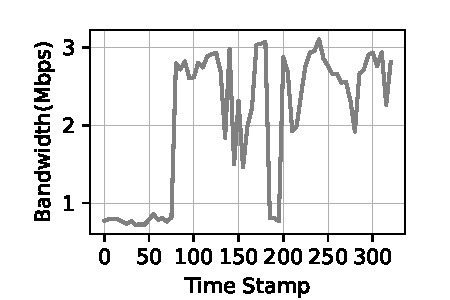
\includegraphics[width=\linewidth]{figures/chap04/evaluation_multialgo/bandwidth_68_plot.pdf}
  \caption{类型1带宽随时间变化}
  \label{type1-band-eva}
\end{subfigure}%
\begin{subfigure}[t]{0.47\linewidth}
  \centering
  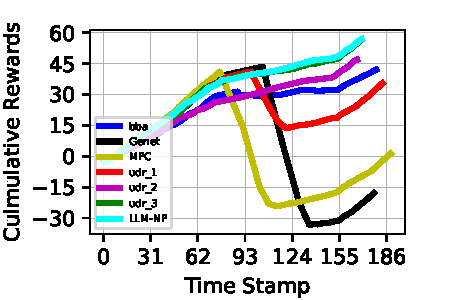
\includegraphics[width=\linewidth]{figures/chap04/evaluation_multialgo/test_68_plot.pdf}
  \caption{类型1下LLM-NP性能表现奖励值}
  \label{type1-rew-eva}
\end{subfigure}

\begin{subfigure}[t]{0.47\linewidth}
  \centering
  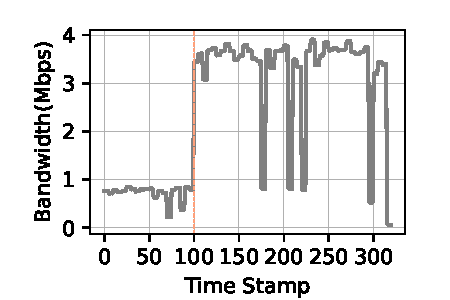
\includegraphics[width=\linewidth]{figures/chap04/evaluation_multialgo/bandwidth_27_plot.pdf}
  \caption{类型2带宽随时间变化}
  \label{type2-band-eva}
\end{subfigure}%
\begin{subfigure}[t]{0.47\linewidth}
  \centering
  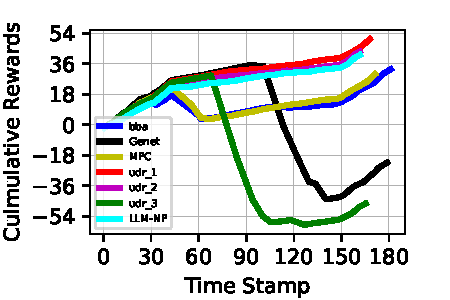
\includegraphics[width=\linewidth]{figures/chap04/evaluation_multialgo/test_27_plot.pdf}
  \caption{类型2下LLM-NP性能表现奖励值}
  \label{type2-rew-eva}
\end{subfigure}

\begin{subfigure}[t]{0.47\linewidth}
  \centering
  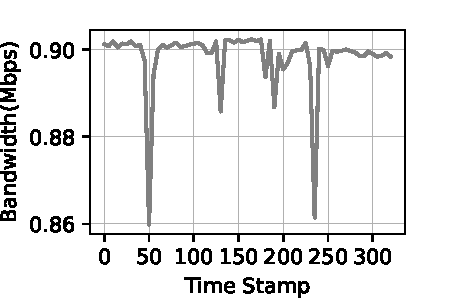
\includegraphics[width=\linewidth]{figures/chap04/evaluation_multialgo/bandwidth_88_plot.pdf}
  \caption{类型3带宽随时间变化}
  \label{type3-band-eva}
\end{subfigure}%
\begin{subfigure}[t]{0.47\linewidth}
  \centering
  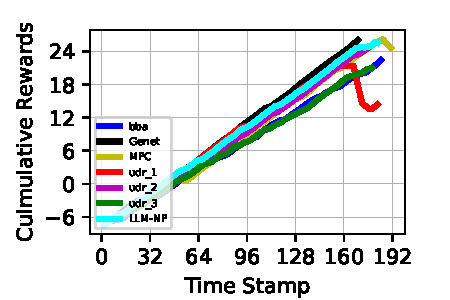
\includegraphics[width=\linewidth]{figures/chap04/evaluation_multialgo/test_88_plot.pdf}
  \caption{类型3下LLM-NP性能表现奖励值}
  \label{type3-rew-eva}
\end{subfigure}

\caption{三个类型网络环境下LLM-NP与传统算法的奖励值对比}
\label{fig:multi-algo-eva}
\end{figure}


图\ref{type1-band-eva}和图\ref{type1-rew-eva}是常见波动带宽情形下LLM-NP的效果呈现。这类带宽的特点是会有较大的抖动和方差,常见于在移动网络下,例如公交上、地铁上等信号不稳定场景。示例中的带宽波形如图\ref{type1-band-eva}所示,包含约310秒的带宽仿真,表示实时可用带宽(纵轴)随着时间消耗(横轴)而呈现出的变化趋势。带宽在90秒、120秒、150秒、190秒左右时刻出现显著波动。在此带宽下对应的策略规划范式和常规无切换策略运行的效果如图\ref{type1-rew-eva}所示,该图描述了式\eqref{eq:abr_cum_reward2}计算出的累计奖励值(纵轴)随着时间消耗(横轴)而呈现出的变化趋势。累计奖励值从0开始计算,并随着每个块(Chunk)的发送开始增减。在公式中,每个块(Chunk)发送时使用的比特率越高,对应的单次奖励值增加的越多。而奖励分数的减少则是因为遇到了缓冲区的重加载(Rebuffer)和码率变换带来的体验下降,其中缓冲区的重加载带来的体验下降更多。在图中,LLM-NP(水绿色点线表示)的奖励值曲线升高平稳,并在最终获得了最高的奖励值;与之形成对比的是MPC、Genet、udr\_1算法在90秒、120秒左右都因为网络突变而产生了较大的奖励值滑落,代表最终用户体验的下降。

图\ref{type2-band-eva} 和 \ref{type2-rew-eva}是网络状况在某一时刻后可用带宽长时变化这一类型下LLM-NP的效果呈现。这类网络的特点是在某一时刻后带宽有所增加或减少。图\ref{type2-band-eva} 中的网络带宽中在100秒出现了显著的长期可用带宽增加。相应地,传统的无法作出切换的算法会在相应带宽变化前后呈现出奖励值的下降,而LLM-NP呈现了较好的稳定性,如图\ref{type2-rew-eva}所示。

图\ref{type3-band-eva} 和 \ref{type3-rew-eva}是网络状况稳定这一类型下LLM-NP的效果呈现。这种情况下,所有的工作范式都保持了比较好的工作性能,LLM-NP呈现了与其他方法一致的最优性能,如图\ref{type3-rew-eva}所示。

\textbf{LLM-NP工作时的运行比特率和算法切换:}为了衡量LLM-NP工作时的性能表现,本研究记录并分析了其在工作时的比特率变化、随时间发送块(Chunk)时获得的单个奖励值、对网络带宽的利用率和在不同算法之间的切换情况,对应情况绘制的图例如图\ref{fig:single-algo-detail}所示。

\begin{figure}[ht]
\centering
\begin{subfigure}[t]{0.47\linewidth}
  \centering
  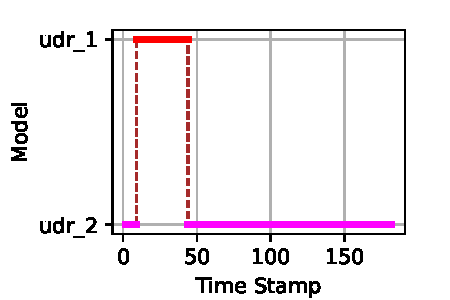
\includegraphics[width=\linewidth]{figures/chap04/evaluation_single_algo_detail/model_88_plot.pdf}
  \caption{LLM-NP工作时中的模型切换状况}
  \label{detail_model_switch}
\end{subfigure}
\begin{subfigure}[t]{0.47\linewidth}
  \centering
  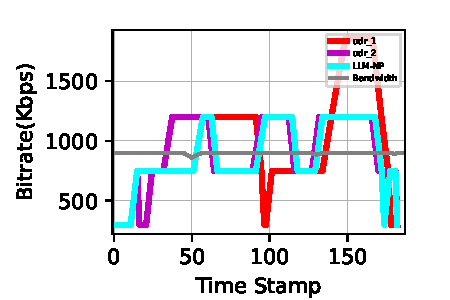
\includegraphics[width=\linewidth]{figures/chap04/evaluation_single_algo_detail/bitrate_88_plot.pdf}
  \caption{LLM-NP工作时比特率}
  \label{detail_bitrate}
\end{subfigure}%

\begin{subfigure}[t]{0.47\linewidth}
  \centering
  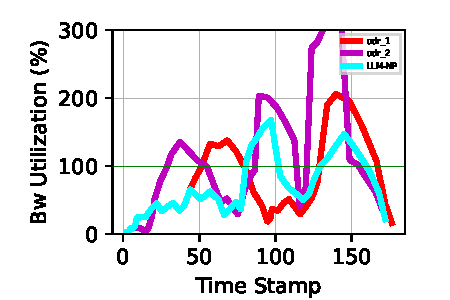
\includegraphics[width=\linewidth]{figures/chap04/evaluation_single_algo_detail/bandwidth_utilization_88_plot.pdf}
  \caption{LLM-NP工作时的带宽利用率}
  \label{detail_bandwid_util}
\end{subfigure}%
\begin{subfigure}[t]{0.47\linewidth}
  \centering
  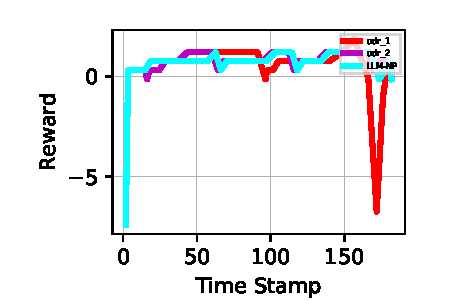
\includegraphics[width=\linewidth]{figures/chap04/evaluation_single_algo_detail/reward_88_plot.pdf}
  \caption{LLM-NP工作获得单次奖励值}
  \label{detail_reward}
\end{subfigure}

\caption{LLM-NP工作时的性能表现细节}
\label{fig:single-algo-detail}
\end{figure}


图\ref{detail_model_switch}表明了LLM-NP在本示例工作时的涉及使用的算法,包括“udr\_1”和“udr\_2”。模型在最初的10秒左右的时间中使用了“udr\_2”算法,随后切换到“udr\_1”,并在接近50秒时又切换回“udr\_2”算法并保持不变。

图\ref{detail_bitrate}代表LLM-NP工作时的发送比特率随着时间推移而选择的块(Chunk)变化值。图中灰色的线代表使用的环境模拟可用带宽,其可用带宽在900Kbps左右保持平稳;草绿色线代表LLM-NP在该任务下的比特率控制。在本次的算法规划中,算法所涉及的两个算法“udr\_1”和“udr\_2”也在图中分别以红色和紫色表示。通过该图,我们可以直观地看到LLM-NP的比特率控制相比使用单一的算法有更优的性能:“udr\_2”的算法在前40秒内的比特率较低,没有完全利用到大部份的带宽,而LLM-NP做出的切换能够有效增加带宽利用率,提升使用性能;而“udr\_1”在100秒后的比特率控制波动较大,存在较大的比特率切换,且较多超过了可用带宽,可能会导致重缓冲(Rebuffer)的产生,和较多比特率切换罚项,造成最终QoE奖励值下降。在本例中,LLM-NP相比任一单一的算法在带宽利用、比特率切换和重加载避免方面表现出了更佳的性能。

图\ref{detail_bandwid_util}代表LLM-NP工作时的带宽利用率。类似的,涉及到切换的算法也相应在图中绘制用于对比和衡量。LLM-NP相比“udr\_1”和“udr\_2”有更稳定的,接近高带宽利用率的性能。图\ref{detail_reward}代表LLM-NP工作时发送每个块(Chunk)时获得的单次奖励值。

\subsection{局限性讨论}
本章节所设计的LLM-NP范式的工作范围限定于具备庞大策略库,且对应系统能够实现运行时切换的网络任务。目前研究能够在自适应码率任务的仿真系统上实现了切换,产生初步的优化效果和相应的性能提升。然而,其效果的进一步提升与验证需要借助更大的数据量和更真实的、大规模的正式系统平台完成验证,包括在更多差异化的网络任务(例如拥塞控制、梯度压缩、实时通信发送率控制)、更全面的算法运行数据采集(多种算法的长时运行数据)、更大的预训练模型(使用更高参数量的模型)上展开验证,以及确定对应的任务在真实系统部署中切换所存在的难点。
\section{本章小结}
本章节提出了LLM-NP,一种用于网络控制的策略规划新范式。这种范式改变了过往在网络传输控制中固定一成不变的策略选择,并利用了大模型的感知和规划能力,为网络传输控制类的任务提供了可动态切换的解决方案。该工作对大模型展开了在网络任务上的具体数据上的微调对齐,并实现了网络规划范式与自适应码率任务的完整交互系统,获得了在变动网络带宽环境下,超越传统单一运行算法的可靠的性能提升案例。

% !TeX root = ../thuthesis-example.tex

\chapter{总结与展望}
\section{研究总结}
在当下的科研与多数互联网通信服务中,如何在复杂网络环境中提升传输效率以及保证服务良好的用户体验是重要的研究问题。合理的传输策略能够有效增加信息传递效率,提升用户对服务的满意程度,降低通信开销和成本,因此设计更高效的传输策略对于内容服务提供商、网络通信运营商和用户受众都发挥着举足轻重的作用,尤其是在诸如网络拥塞控制、自适应视频码率、实时通信系统发送速率控制等任务上具有非常可观的优化收益。本文的研究旨在结合最新的人工智能决策模型来优化这类任务中的传输策略,通过精细化具体传输内的网络场景和用户偏好展开策略和工作范式的优化。

本文通过从应用场景需求异质性和环境性能适配差异性两个角度展开研究。对于应用场景需求异质性,研究选定了云游戏下实时传输速率控制场景,对算法展开优化。本文认为,不同的场景中延迟对用户满意度的影响存在差异,因此通过测量获得具体的“敏感度”。研究首先针对云游戏中不同的游戏场景展开了大规模的时延与使用时长关系的数据测量并进行了时延对应的用户满意度主观打分实验,获得了场景下真实的用户反馈。为将上述的用户反馈数据应用至算法设计中,本工作使用最小二乘估计将每个场景下的数据映射为连续的敏感性函数,获得了多条不同的敏感性曲线。在实时传输速率控制上使用强化学习的框架完成交互,并将前获得敏感性曲线应用在强化学习的奖励函数,获得匹配场景实际需求的控制策略。

对于环境性能适配差异性,本文通过构建一个工作在策略之上的范式,避免网络控制策略陷入到局部最优而非全局最优解中,进而增强差异化的网络环境下的传输整体性能。研究首先通过更新网络任务与策略规划系统的策略选择和交互机制增加了切换机制,然后构建策略规划系统。策略规划系统利用预训练模型强大的规划能力作判断,并采用了序列化的决策模型适配模型的嵌入层。为了进一步对齐模型的规划输入输出,使用预采集的数据完成了离线强化学习模型权重的调优,并在自适应码率上展开了案例研究,为多种网络任务提供了一个新的网络规划范式。

综上所述,本文借助人工智能决策的框架和模型完成了一个云游戏场景下的传输策略优化和一个网络控制策略的选择范式,能够针对于异质化的网络场景提供差异化的码率决策,提升了网络利用率;同时网络控制策略的选择范式能够避免单一的算法在变动的网络环境中因长期工作而陷入次优解。本文提出的两个模块独立工作,能够在整个传输过程中和多种应用中提供更优异的性能。

\section{未来展望}
本文针对于异质网络场景下的网络传输任务展开了较为深入的探究。随着该问题引起越来越多的关注,该领域仍然存在较大的研究空间,包括以下两个改进方向:

(1) 场景下弱用户参考基准的时延敏感度的获取及泛化

尽管使用敏感度曲线细分的场景能够有效地提高传输效率、增加用户体验以及降低成本,当前工作对于时延敏感度评估的过程仍需高度依赖人类主观偏好的反馈,而开展大量此类的时延和测量是极大的成本开销,且测量的结果只能适用于极小一部分场景,例如本研究中时间和空间变换度值接近的场景。因此,将时延敏感度进一步与人类直接的打分解耦合能够加强场景化算法的应用,这可以通过多种方式实现:使用具有强代表性的无参考指标,例如Deep-BVQM \cite{jamshidi2022deep} 使用无参考指标PSNR的方式实现了视频帧级别的质量预测;或是借助诸如大模型智能体(LLM Agent)的新人工智能技术,通过少量采集数据即可构建敏感度映射关系,并将相关数据映射到更多差异化场景下。

(2) 网络规划范式规划结果的可解释性与配置

本文现阶段设计的网络规划范式决策模型能够作出策略的规划,但仍然存在进一步优化的空间。针对于大多网络要求的即时性和简明性,现有的工作范式未能阐明其规划和决策的原因。而大语言模型本身具有强大的自然语言能力,便于以人类易于理解的方式展开阐述。如何利用该种能力对网络规划范式规划结果进行解释,乃至进一步对选定策略的配置项展开配置是重要的未来研究方向,它将透明化大模型决策过程并进一步优化配置性能,提升配置能力。透明化的另一个好处是便于模型的蒸馏,降低后续的长期部署成本。

% 其他部分
\backmatter

% 参考文献
\bibliography{ref/refs}  % 参考文献使用 BibTeX 编译
% \printbibliography       % 参考文献使用 BibLaTeX 编译

% 附录
% 本科生需要将附录放到声明之后,个人简历之前
\appendix
% % !TeX root = ../thuthesis-example.tex

\begin{survey}
\label{cha:survey}

\title{Title of the Survey}
\maketitle


\tableofcontents


本科生的外文资料调研阅读报告。


\section{Figures and Tables}

\subsection{Figures}

An example figure in appendix (Figure~\ref{fig:appendix-survey-figure}).

\begin{figure}
  \centering
  \includegraphics[width=0.6\linewidth]{example-image-a.pdf}
  \caption{Example figure in appendix}
  \label{fig:appendix-survey-figure}
\end{figure}


\subsection{Tables}

An example table in appendix (Table~\ref{tab:appendix-survey-table}).

\begin{table}
  \centering
  \caption{Example table in appendix}
  \begin{tabular}{ll}
    \toprule
    File name       & Description                                         \\
    \midrule
    thuthesis.dtx   & The source file including documentation and comments \\
    thuthesis.cls   & The template file                                   \\
    thuthesis-*.bst & BibTeX styles                                       \\
    thuthesis-*.bbx & BibLaTeX styles for bibliographies                  \\
    thuthesis-*.cbx & BibLaTeX styles for citations                       \\
    \bottomrule
  \end{tabular}
  \label{tab:appendix-survey-table}
\end{table}


\section{Equations}

An example equation in appendix (Equation~\eqref{eq:appendix-survey-equation}).
\begin{equation}
  \frac{1}{2 \uppi \symup{i}} \int_\gamma f = \sum_{k=1}^m n(\gamma; a_k) \mathscr{R}(f; a_k)
  \label{eq:appendix-survey-equation}
\end{equation}


\section{Citations}

Example\cite{dupont1974bone} citations\cite{merkt1995rotational} in appendix
\cite{dupont1974bone,merkt1995rotational}.


% 默认使用正文的参考文献样式;
% 如果使用 BibTeX,可以切换为其他兼容 natbib 的 BibTeX 样式。
\bibliographystyle{unsrtnat}
% \bibliographystyle{IEEEtranN}

% 默认使用正文的参考文献 .bib 数据库;
% 如果使用 BibTeX,可以改为指定数据库,如 \bibliography{ref/refs}。
\printbibliography

\end{survey}
       % 本科生:外文资料的调研阅读报告
% % !TeX root = ../thuthesis-example.tex

\begin{translation}
\label{cha:translation}

\title{书面翻译题目}
\maketitle

\tableofcontents


本科生的外文资料书面翻译。


\section{图表示例}

\subsection{图}

附录中的图片示例(图~\ref{fig:appendix-translation-figure})。

\begin{figure}
  \centering
  \includegraphics[width=0.6\linewidth]{example-image-a.pdf}
  \caption{附录中的图片示例}
  \label{fig:appendix-translation-figure}
\end{figure}


\subsection{表格}

附录中的表格示例(表~\ref{tab:appendix-translation-table})。

\begin{table}
  \centering
  \caption{附录中的表格示例}
  \begin{tabular}{ll}
    \toprule
    文件名          & 描述                         \\
    \midrule
    thuthesis.dtx   & 模板的源文件,包括文档和注释 \\
    thuthesis.cls   & 模板文件                     \\
    thuthesis-*.bst & BibTeX 参考文献表样式文件    \\
    thuthesis-*.bbx & BibLaTeX 参考文献表样式文件  \\
    thuthesis-*.cbx & BibLaTeX 引用样式文件        \\
    \bottomrule
  \end{tabular}
  \label{tab:appendix-translation-table}
\end{table}


\section{数学公式}

附录中的数学公式示例(公式\eqref{eq:appendix-translation-equation})。
\begin{equation}
  \frac{1}{2 \uppi \symup{i}} \int_\gamma f = \sum_{k=1}^m n(\gamma; a_k) \mathscr{R}(f; a_k)
  \label{eq:appendix-translation-equation}
\end{equation}


\section{文献引用}

附录\cite{dupont1974bone}中的参考文献引用\cite{merkt1995rotational}示例
\cite{dupont1974bone,merkt1995rotational}。


\appendix

\section{附录}

附录的内容。


% 书面翻译的参考文献
% 默认使用正文的参考文献样式;
% 如果使用 BibTeX,可以切换为其他兼容 natbib 的 BibTeX 样式。
\bibliographystyle{unsrtnat}
% \bibliographystyle{IEEEtranN}

% 默认使用正文的参考文献 .bib 数据库;
% 如果使用 BibTeX,可以改为指定数据库,如 \bibliography{ref/refs}。
\printbibliography

% 书面翻译对应的原文索引
\begin{translation-index}
  \nocite{mellinger1996laser}
  \nocite{bixon1996dynamics}
  \nocite{carlson1981two}
  \bibliographystyle{unsrtnat}
  \printbibliography
\end{translation-index}

\end{translation}
  % 本科生:外文资料的书面翻译
% % % !TeX root = ../thuthesis-example.tex

% \chapter{补充内容}


% \section{大规模数据测量中的数据属性及筛选方法}\label{shaixuan}


% 被测量的游戏及每款游戏使用的数据集如表\ref{table_flow_count}所示。数据有两种不同粒度类型:流粒度持续时间是指从用户发起连接请求开始,直到用户关闭连接为止,形成一组统计数据为一次统计,作为单条数据进行使用的数据;而帧粒度持续时间则是指单个流中每一帧画面显示为一次统计,一个流形成一张表格。后者的粒度比前者更细,可以获得更多细节统计信息,收集用于进一步探索,两者共同使用形成测量结果。
% \begin{table}[ht]
\centering
\caption{用于统计游戏的流属性统计}
\begin{tabular}{@{}ccccc@{}}
\toprule
\textbf{游戏}        & \textbf{流粒度持续时间(小时)} & \textbf{帧粒度持续时间(小时)} \\ \midrule
2D-RPG I             & 3707.74                  & 910.23                    \\
2D-RPG III           & 2558.73                  & 460.17                    \\
3D-RPG I             & 889.68                   & 49.83                     \\
动作游戏 I           & 1194.60                  & 102.73                    \\
A-RPG I              & 529.15                   & 87.37                     \\
休闲游戏 I           & 70.47                    & 3.29                      \\
CCG I                & 200.42                   & 12.80                     \\
FPS I                & 1360.89                  & 277.21                    \\
FPS II               & 151.32                   & 79.51                     \\
FPS III              & 570.81                   & 62.75                     \\
FPS IV               & 281.95                   & 20.71                     \\
MMORPG I             & 638.79                   & 82.72                     \\
MOBA I               & 685.65                   & 378.66                    \\
MOBA II              & 247.16                   & 98.07                     \\
运动游戏 I           & 1068.06                  & 249.90                    \\
运动游戏 II          & 155.76                   & 35.31                     \\
运动游戏 III         & 1376.29                  & 0.13                      \\
TPS I                & 331.30                   & 25.43                     \\ \bottomrule
\end{tabular}
\label{table_flow_count}
\end{table}


% 从大规模测量中获得的原始数据,由于记录中存在异常使用数据,往往偏离理想数据。为了确保数据测量的准确性,需要应用某些规则,尽可能排除由于用户或设备链路问题导致的异常数据。可能的异常数据情况包括:


% \begin{itemize} 
% \item \textbf{用户提前退出:}该情况指的是用户与服务器建立连接后,但未实际进行游戏便退出。此类连接通常持续时间较短,不超过 2 分钟。 

% \item \textbf{僵尸流量:}该情况指的是客户端与服务器的连接异常断开,但流量未停止并继续计数,导致数据不正确。这样可能导致流量被计量几个小时甚至超过一天,超过了正常可接受的长时间使用时长。 

% \item \textbf{频繁切换网络:}为了排除用户网络连接不稳定的情况,我们选择常见的网络类型(2.4GHz 和 5GHz Wi-Fi、以太网或蜂窝数据)。在单次连接中,频繁切换网络链接的情况将不被纳入统计。 

% \item \textbf{极低的实际编码比特率:}实际编码比特率低于设置比特率的十分之一,通常是由于长时间静态或极小的画面,导致需要传输的残余信息非常少,从而导致极低的比特率。这表明尽管用户已连接,但并未进行任何操作。 

% \item \textbf{低交互频率}:用户客户端接收到的输入频率极低,如键盘、鼠标或游戏手柄的输入频率。此类情况也表明用户已建立连接,但未进行任何游戏活动。 

% \item \textbf{异常的客户端处理时间:}通常,在性能稳定的机器上接收和解码视频不应超过某个时间限制。处理时间波动较大或连接时间过长的情况也应排除。在处理延迟过高的情况下,用户无法正常游戏,而连接时间过长则表明客户端存在异常行为,因此需要排除。 


% \end{itemize}

% 致谢
% !TeX root = ../thuthesis-example.tex

\begin{acknowledgements}
四季流转,转眼间就来到了我硕士生涯的尾声。回顾过去,有许多记忆犹新的片段依然历历在目,它们就像拼图一样构成了完整的三年。我感到幸运,因为一路上有许多无声支持与陪伴,伴我走过或是快乐的,或是具有压力的日子。因此,我想在此致谢:

衷心感谢我的导师王智副教授,感谢您在整个研究生的过程中提供的悉心指导与鼓励。在三年多的时间里,您深刻并富有远见的见解、专业的行事和深厚的累积就像是在科技的浪潮和风暴中的一座灯塔,让我看到应该探索的朝向。您不仅给予了学术上的入门与启发,还提供了许多与真实工业与学术界接触的宝贵机会,在此期间学会了与不同业界的人展开合作和沟通。更重要的是,在您的言传身教下,我学会了严谨与高效的做事态度与方法,以及良好的面对挑战的心态。这些习惯和心态将会伴随我受益终身。

感谢现在于腾讯进行技术研究的吴成磊大师兄和字节跳动的张伟技术专家,你们的指导和经验引领我在相关的专业领域上有更深刻的认识,实践的技术上更加精通。

感谢MMLab实验室中的所有成员,感谢24级博士吴铎为我带来了新的灵感与启发,并给予详细的指导。感谢20级硕士(24级博士)解书照,给予我一直以来默默的帮助。感谢21级硕士代诗绮,你的努力和行事方式一直激励着我,科研的思路也让我有所启发。感谢21级硕士(24级博士)路荣伟提供的科研学习的机会。感谢LM小组的王瀞禾、孙乐、王智民、张晏宁,我们共同学习和进步。我还想感谢22级同级的同学刘文洋、邹岷强、闫柏旭、卢美子,23级姜佳成在研一研二期间经常的鼓励和一同游玩解压的快乐时光。感谢23级博士李也、22级硕士李迎欣在Retreat会议中结下的深厚友谊和难忘时光。感谢22级同级同学杜南洋、张伟翔、姚为、张岑岳、张露丹、方子介,我们共同努力,互相帮助面对各种挑战。感谢23级师弟葛士嘉、张瑾睿、宋佳俊、蒋沁廷、李群、李孝杰曾一起游玩放松。24年,又有许多新生加入,我们共同参与了MMLab年会,在此中认识了充满活力的新人,共同度过了意犹未尽和不舍离开的时光。

感谢我的父母,你们是我最坚实和实在的后盾,在生活上无微不至的关心和对我无私的付出令我感动,这让我能够毫无后顾之忧地不断追寻自己的梦想。感谢我的女朋友,这么多年的异地你不曾放弃,在许多个困难的瞬间都是你重新给予我力量。

我还想感谢清华给予的广阔平台和优渥资源。清华所拥有的凝聚力让我受到许多受益匪浅的帮助;其校训精神和价值观也深刻地感化并滋润着我们,激励我们不负社会,警记优渥的环境下所塑造的能力优势的意义是用于帮助有需要的人。

最后,我想感谢自己的努力和梦想。在一个努力既有回报的时代下,相信每个人都会或早或晚得到奖赏。但即使有一天,回报不再显著,我们会庆幸和真诚地感谢那些黄金岁月。


\end{acknowledgements}


% 声明
% 本科生开题报告不需要
\statement
% 将签字扫描后的声明文件 scan-statement.pdf 替换原始页面
% \statement[file=scan-statement.pdf]
% 本科生编译生成的声明页默认不加页脚,插入扫描版时再补上;
% 研究生编译生成时有页眉页脚,插入扫描版时不再重复。
% 也可以手动控制是否加页眉页脚
% \statement[page-style=empty]
% \statement[file=scan-statement.pdf, page-style=plain]

% 个人简历、在学期间完成的相关学术成果
% 本科生可以附个人简历,也可以不附个人简历
% !TeX root = ../thuthesis-example.tex

\begin{resume}

  \section*{个人简历}

  2000 年 8 月 27 日出生于上海市静安区。

  2018 年 9 月考入中国传媒大学大学信息与通信工程学院广播电视工程专业,2022 年 6 月本科毕业并获得工学学士学位。

  2022 年 9 月免试进入清华大学深圳国际研究生院攻读计算机专业硕士至今。


  \section*{在学期间完成的相关学术成果}

  \subsection*{学术论文}

  \begin{achievements}
    \item \textbf{Xuanyu Zhu}, Shuzhao Xie, Zhi Wang.Sense: Latency Sensitivity-Aware RL Rate Control for Cloud Gaming[C]. Proceedings of the 33nd ACM International Conference on Multimedia. 2025. (CCF-A, under review)
    
    \item \textbf{Xuanyu Zhu}, Duo Wu, Wei Zhang, Zhi Wang. Network Task Policy Selection Based on Large Language Models[C]. The 9th Asia-Pacific Workshop on Networking (APNET'25). (CCF-C, under review)
    
    \item Shiqi Dai, \textbf{Xuanyu Zhu}, Naiqi Li, Zhi Wang. Procedural level generation with diffusion models from a single example[C]. Proceedings of the AAAI Conference on Artificial Intelligence. 2024, 38(9): 10021-10029. (CCF-A)

  \end{achievements}
\end{resume}


% 指导教师/指导小组评语
% 本科生不需要
% !TeX root = ../thuthesis-example.tex

\begin{comments}
% \begin{comments}[name = {指导小组评语}]
% \begin{comments}[name = {Comments from Thesis Supervisor}]
% \begin{comments}[name = {Comments from Thesis Supervision Committee}]

  论文提出了……

\end{comments}


% 答辩委员会决议书
% 本科生不需要
% !TeX root = ../thuthesis-example.tex

\begin{resolution}

  论文提出了……

  论文取得的主要创新性成果包括:

  1. ……

  2. ……

  3. ……

  论文工作表明作者在×××××具有×××××知识,具有××××能力,论文××××,答辩××××。

  答辩委员会表决,(×票/一致)同意通过论文答辩,并建议授予×××(姓名)×××(门类)学博士/硕士学位。

\end{resolution}


% 本科生的综合论文训练记录表(扫描版)
% \record{file=scan-record.pdf}

\end{document}
